%\documentclass[handout,xcolor=dvipsnames]{beamer}
\documentclass[xcolor=dvipsnames]{beamer}

\usepackage{pgfpages}
%\mode<handout>{\pgfpagesuselayout{4 on 1}[letterpaper,border shrink=5mm,landscape]}
\mode<presentation>{
  \setbeamertemplate{navigation symbols}{}
  %\setbeamertemplate{caption}{\raggedright\insertcaption\par}
  %\setbeamertemplate{caption}[numbered]
}

\usepackage[export]{adjustbox}
\usepackage{graphicx}
\usepackage{algorithm,algorithmic}
\usepackage{multirow}
%\usepackage{cancel}
\usepackage{booktabs} % for midrule
\usepackage{subfig}
\usepackage{tikz}
\usetikzlibrary{shadows,arrows,decorations.pathmorphing,backgrounds,positioning,fit,petri,fadings,shapes,calc,shapes.multipart}

\usepackage{scalefnt}
\usepackage{appendixnumberbeamer}

\usepackage{bbm}
\usepackage{natbib}

\usetheme{Boadilla}

\newcommand{\exclude}[1]{}
\newcommand{\modulus}[1]{\left| #1 \right|}
\newcommand{\norm}[1]{\left\Vert #1 \right\Vert}
\newcommand{\function}[3]{#1 : #2 \mapsto #3}
\newcommand{\real}{\mathbb{R}}
\newcommand{\set}[2]{\left\{ #1 : #2 \right\}}
\newcommand{\ip}[2]{\left< #1 , #2 \right>}
\newcommand{\T}{\mathcal{T}}
\newcommand{\N}{\mathcal{N}}
\newcommand{\I}{\mathcal{I}}
\newcommand{\C}{\mathcal{C}}
\newcommand{\ds}{\displaystyle}
\newcommand{\rec}{\mathrm{rec}}
\renewcommand{\int}[1]{\mathrm{int}(#1)}
\newcommand{\im}[1]{\mathrm{im}(#1)}
\newcommand{\ri}[1]{\mathrm{rint}(#1)}
\newcommand{\dom}[1]{\mathrm{dom}(#1)}
\newcommand{\dual}[1]{#1^D}

\newcommand{\cA}{\mathcal{A}}
\newcommand{\cD}{\mathcal{D}}
\newcommand{\cN}{\mathcal{N}}
\newcommand{\cL}{\mathcal{L}}
\newcommand{\cP}{\mathcal{P}}
\newcommand{\Mu}{\mathcal{M}}

\newcommand{\VI}{\textsc{VI}}
\newcommand{\PATH}{\textsc{Path}}
\newcommand{\EMP}{\textsc{Emp}}
\newcommand{\SELKIE}{\textsc{Selkie}}
\newcommand{\SOL}{\textsc{SOL}}
\newcommand{\st}{\mathrm{s.t.} \hspace*{1pt}}
\newcommand{\Real}{\mathbb{R}\cup\{\infty\}}
\newcommand{\expect}{\mathbb{E}}
\newcommand{\risk}{\rho}
\newcommand{\A}{\mathcal{A}}
\newcommand{\F}{\mathcal{F}}
\newcommand{\cQ}{\mathcal{Q}}
\newcommand{\argmin}{\mathrm{argmin}}
\newcommand{\argmax}{\mathrm{argmax}}
\newcommand{\cvar}{CVaR}
\newcommand{\cvarlo}{\underline{\cvar}}
\newcommand{\cvarup}{\overline{\cvar}}
\newcommand{\Q}{\mathcal{Q}}
\newcommand{\D}{\mathcal{D}}
\newcommand{\EC}{\mathcal{S}}
\newcommand{\black}[1]{{\color{black} #1}}
\newcommand{\red}[1]{{\color{red} #1}}
\newcommand{\blue}[1]{{\color{blue} #1}}
\newcommand{\green}[1]{{\color{OliveGreen!100} #1}}
\newcommand{\purple}[1]{{\color{purple} #1}}
\newcommand{\orange}[1]{{\color{orange} #1}}

%\newcommand{\R}{\Psi}
%\newcommand{\PTDF}{\mathcal{H}}
%\newcommand{\LOOP}{\mathcal{L}}
\newcommand{\MCP}{\text{MCP}}

% \renewcommand{arraystretch}{1.4}
\newenvironment{mytikzpicture}{\noindent\ignorespaces\begin{tikzpicture}}{\end{tikzpicture}\ignorespacesafterend}
\tikzstyle{sensor}=[draw, fill=blue!20, text width=5em,
    text centered, minimum height=2.5em,drop shadow]
\tikzstyle{ann} = [above, text width=5em, text centered]
\tikzstyle{wa} = [sensor, text width=5em, fill=red!20,
    minimum height=3em, rounded corners, drop shadow]
\tikzstyle{sc} = [sensor, text width=13em, fill=red!20,
    minimum height=10em, rounded corners, drop shadow]
\tikzstyle{notimpl}=[draw, semitransparent, fill=blue!20, text width=5em,
text centered, minimum height=2.5em]%,drop shadow]
\def\blockdist{2}
\def\edgedist{2.5}
\tikzset{vfill/.style={color=black,text=black,fill=red!10!gray!30!blue!50,line width=4pt}}

\title[Werewolf]
{Werewolf and NetZero: the interactions between operations, planning, investments and policies}
\author[Ferris (Wisconsin)]{Michael C. Ferris\\ (Joint work with Josh
  Arnold, Adam Christensen and Andy
  Philpott)}
\institute[]{\alert{Jacques-Louis Lions Chair, and Stephen Kleene Professor of Computer
    Science}\\\alert{Computer Sciences Department and}\\ \alert{Wisconsin Institute for Discovery, University of Wisconsin,
    Madison}}
\date[Thompson CPL support]{Wisconsin Public Utility Institute, Board
  Meeting, \\ Madison, March 10, 2020\\
Supported by Tommy G. Thompson Center on Public Leadership}

\begin{document}
\setbeamertemplate{caption}{\raggedright\insertcaption\par}
%
\begin{frame}
  \titlepage
\end{frame}

\section{Introduction}

\begin{frame}
  \frametitle{Jacinda's 2017 election deal}

  \begin{itemize}
  \item Introduce a Zero Carbon Act and establish an independent Climate Commission.
  \item Request the Climate Commission to plan the transition to 100\% renewable electricity by 2035 (which includes geothermal) in a normal hydrological year.
  \item Stimulate up to \$1 billion of new investment in low carbon
    industries by 2020, kick-started by a Government-backed Green
    Investment fund of \$100M.
    \end{itemize}
(Confidence and Supply Agreement between the New Zealand Labour Party
and the Green Party of Aoteoroa)

\alert{Built model GEMSTONE that was used by New Zealand Climate Commission
to help inform this policy}

\end{frame}

\begin{frame}
  \frametitle{New Zealand (NetZero)}

  \begin{columns}[T]
    \begin{column}{0.4\linewidth}
      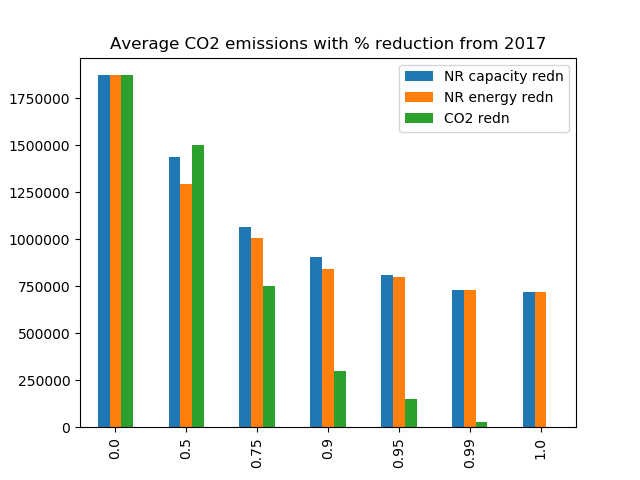
\includegraphics[width=\textwidth]{includes/TotalCarbonv20.png}
%  Since (renewable) geothermal and CCS emit some CO2 100\% renewable yields modest reductions in CO2 emissions.
      \\
      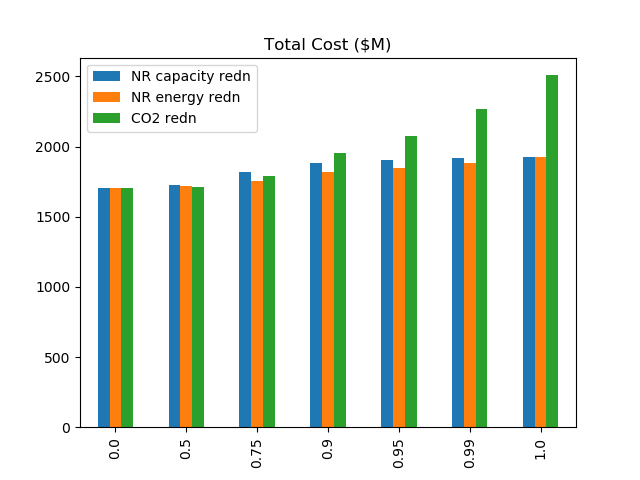
\includegraphics[width=\textwidth]{includes/TotalCostMv20.png}
%  Cost of actually reaching zero CO2 emissions (without geothermal or CCS) increases as we approach the limit.
    \end{column}

    \begin{column}{0.6\linewidth}
      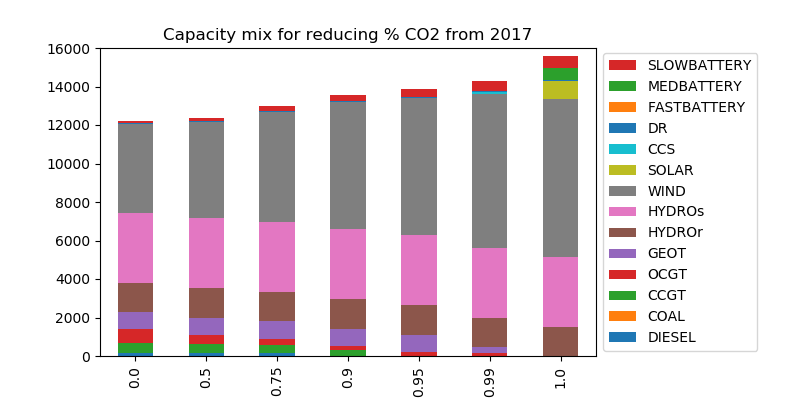
\includegraphics[width=\textwidth]{includes/Sco2rednv20.png}
      % includes/TotalCarbonASv20.png}
      \begin{itemize}
      \item Policies matter: affects reduction amounts and cost
      \item Portfolio of required technologies becomes complex as
        reduction increases
      \item Uncertainties and incentives key
      \item November 2019 climate act provides framework
      \end{itemize}
    \end{column}
  \end{columns}

\end{frame}


\exclude{
    Who are we, what are we doing.

  If we think of the goal for this talk as two-fold:  1) to describe
  WEREWOLF and 2) to pique their interest to participate in the policy
  discussion.

I would recommend to keep it high-level description to start and focus on the value proposition to ask them for their involvement.  They can ask you more detailed questions about the model in the Q\&A afterwards if they are interested.

I like the flow so far and the outputs in slides 6-10.  Although, I think we don't need to show them outputs for this meeting, as it is more of a briefing on WEREWOLF, where we are going with it and inviting them to participate if they are interested.

To gather their interest, we should focus on the value proposition for WEREWOLF to help guide government policy and, to some extent, utility investment decisions based on that policy.
}

\begin{frame}
  \frametitle{Werewolf (Wisconsin Expansion of Renewable Electricity with Optimization under Long-term Forecasts)}

  \centering
  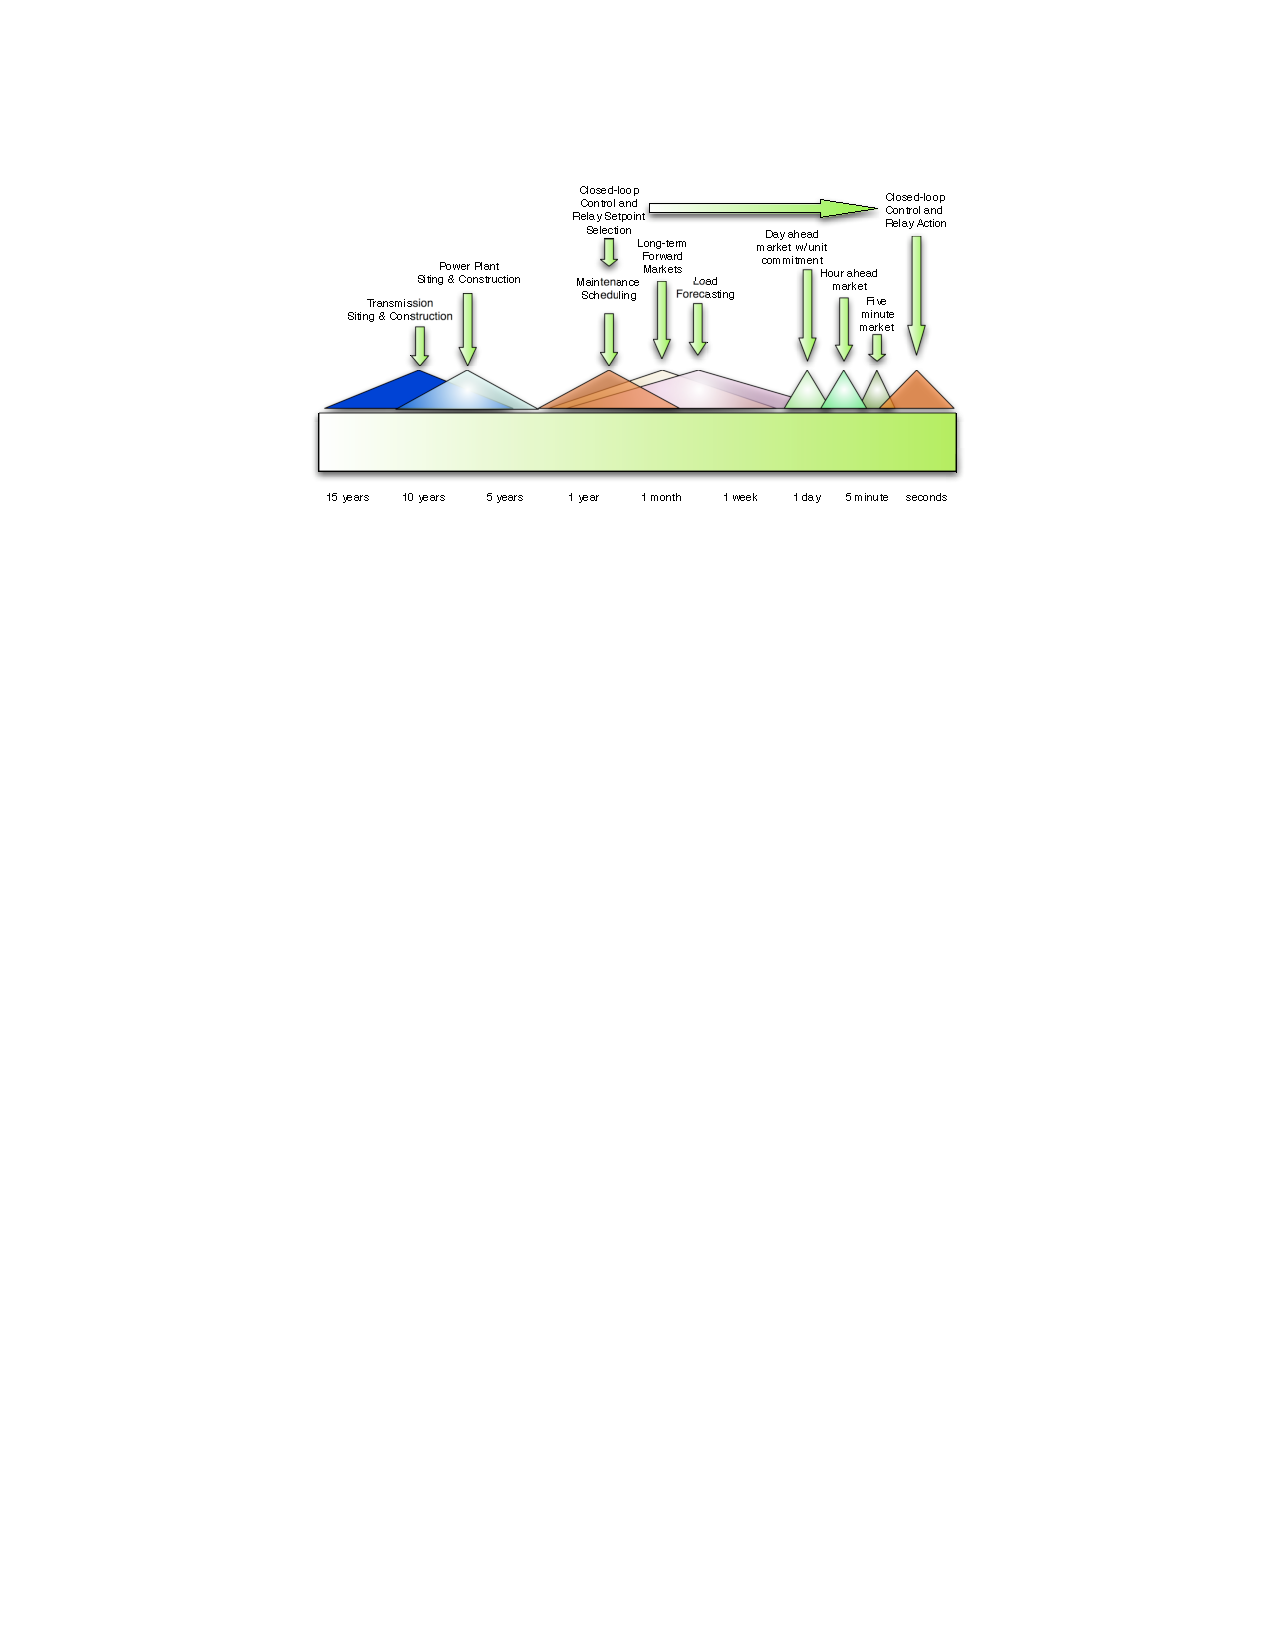
\includegraphics[width=0.8\textwidth]{includes/timescales.pdf}

  \begin{itemize}
  \item Design/policy decisions affecting operations/reliability and vice-versa
  \item Goal: to help policy and decision makers ...
    \begin{itemize}
    \item to distinguish between objectives and actions;
    \item to understand effects of uncertainty;
    \item to understand effects of incentives;
    \item to explore larger design space.
    \end{itemize}
  \end{itemize}

\end{frame}

\begin{frame}
\frametitle{Simplified two-stage stochastic optimization model}
\begin{itemize}
\item Capacity decisions are $z$ at cost $K(z)$
\item Operating decisions: generation $y$ at cost $C(y)$,
loadshedding $q$ at cost $Vq$.
\item Scenarios (futures) $\omega$, demand (load curve) is $d(\omega)$.
\item Minimize capital cost plus expected operating cost:
\end{itemize}
\begin{center}
$%
\begin{array}{rrcl}
\min & \quad K(z)  & + & \expect_{\omega }[%
C(y(\omega )) + Vq(\omega)] \\[1em]
\text{s.t.} & \quad
\textcolor{black}{y(\omega)} & \textcolor{black}{\leq} & %
\textcolor{black}{z} \\
& \textcolor{black}{y(\omega) + q(\omega)} & \textcolor{black}{\geq} & %
                                                                       \textcolor{black}{d(\omega)}
  \\
& (z, y, q) & \in & X
\end{array}%
$
\end{center}
\begin{itemize}
\item WEREWOLF populated using data from Wisconsin: develop the model
  for MISO and look at Wisconsin policies in particular
\item Data and structure facilitate any US regional model
\end{itemize}
\end{frame}

\begin{frame}
  \frametitle{The data}

\begin{itemize}
  \item WEREWOLF is data rich (EPA NEEDS/Integrated Planning Model, NREL ReEDS model data, NREL Annual Technology Baseline)
% I don't know how to make a super nice grid of images here... just putting in the links to images that could go on this slide... needs some help
  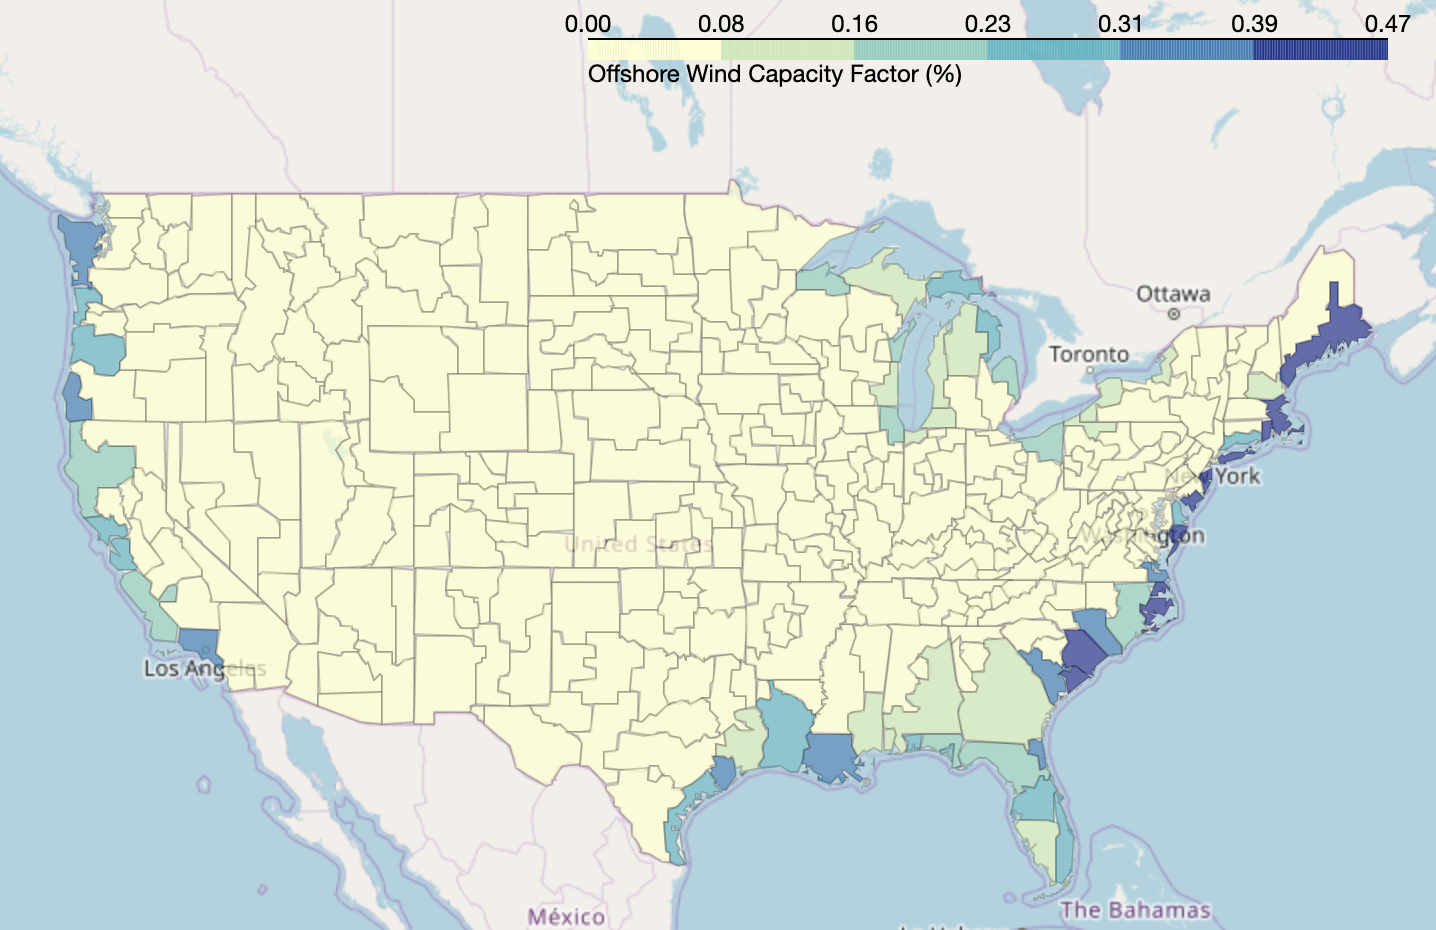
\includegraphics[width=0.25\textwidth]{includes/data_offshore_wind.png}\hspace*{0.2in}
  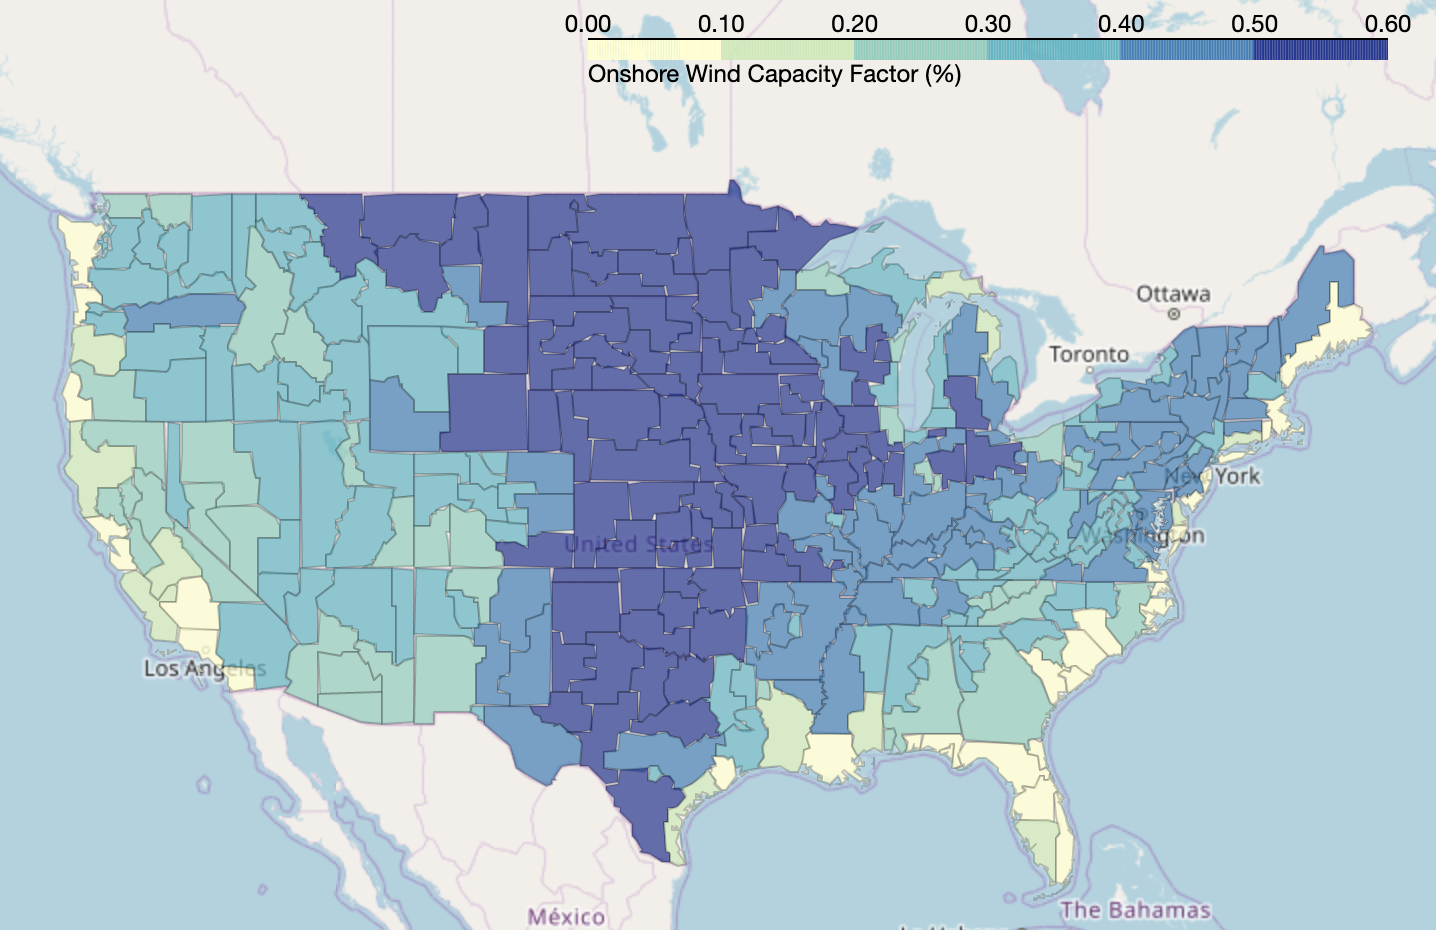
\includegraphics[width=0.25\textwidth]{includes/data_onshore_wind.png}\hspace*{0.2in}
  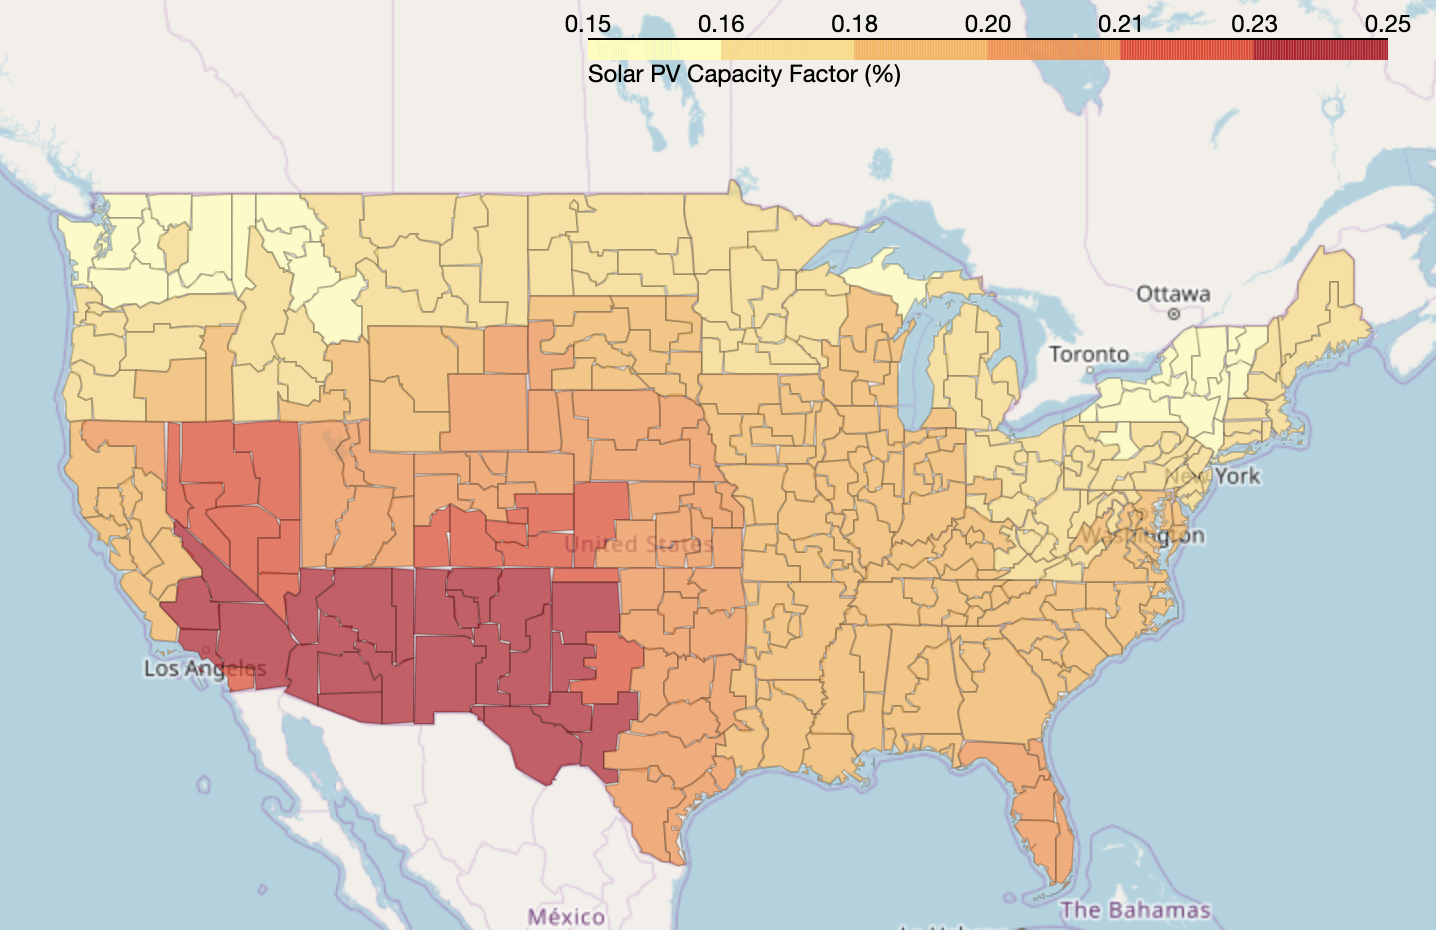
\includegraphics[width=0.25\textwidth]{includes/data_solar.png}
  \item Data is downscaled to county level - \emph{user can customize regions as aggregations of these counties}
  \item Spatial impacts are captured in visualizations
\end{itemize}
\centering
  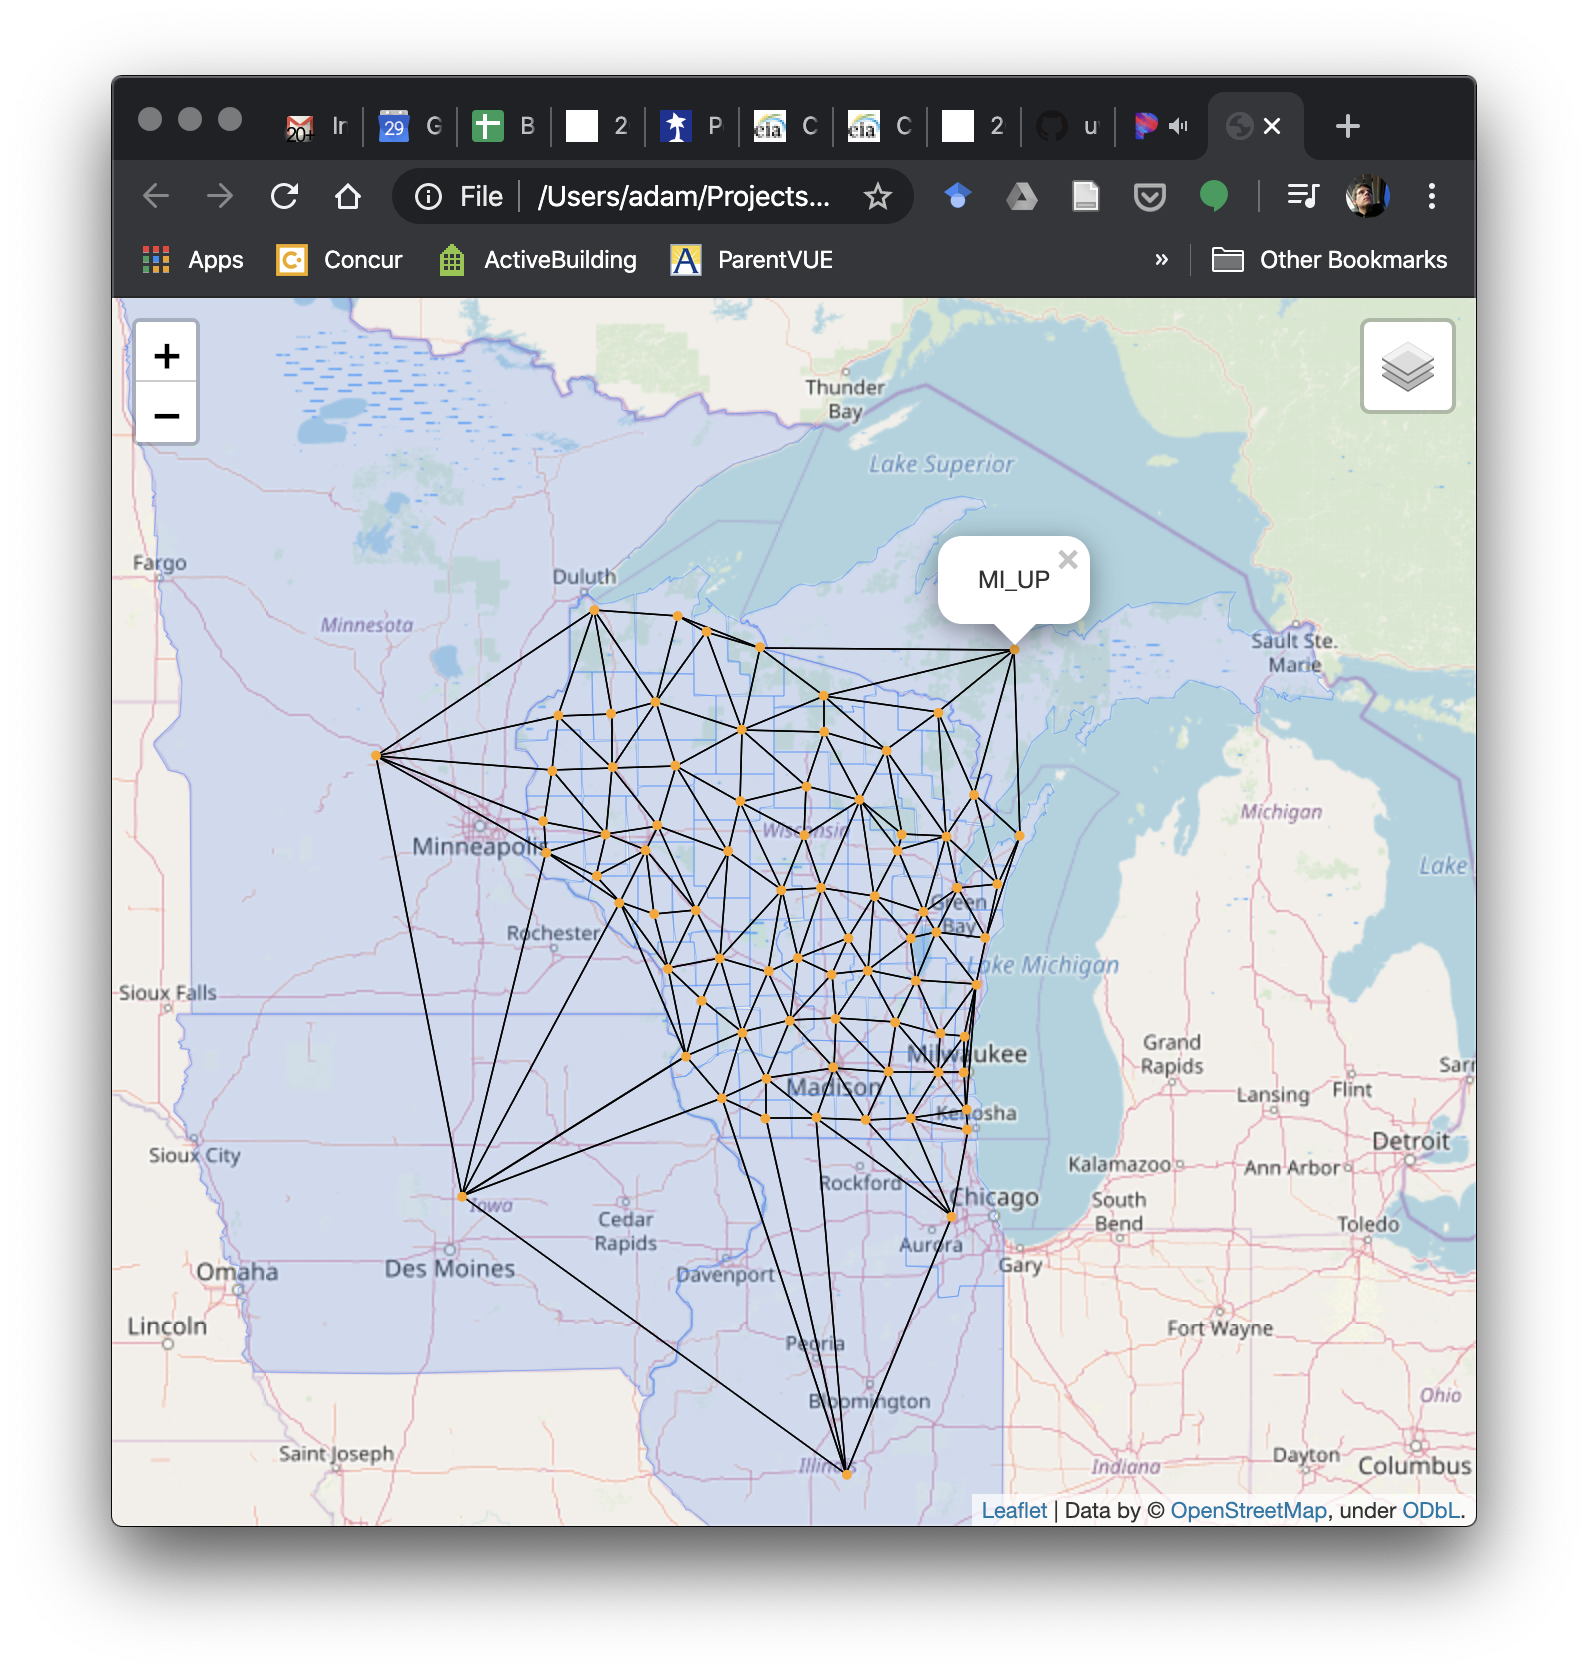
\includegraphics[width=0.30\textwidth]{includes/data_network_browser_view.png}\hspace*{0.2in}
%  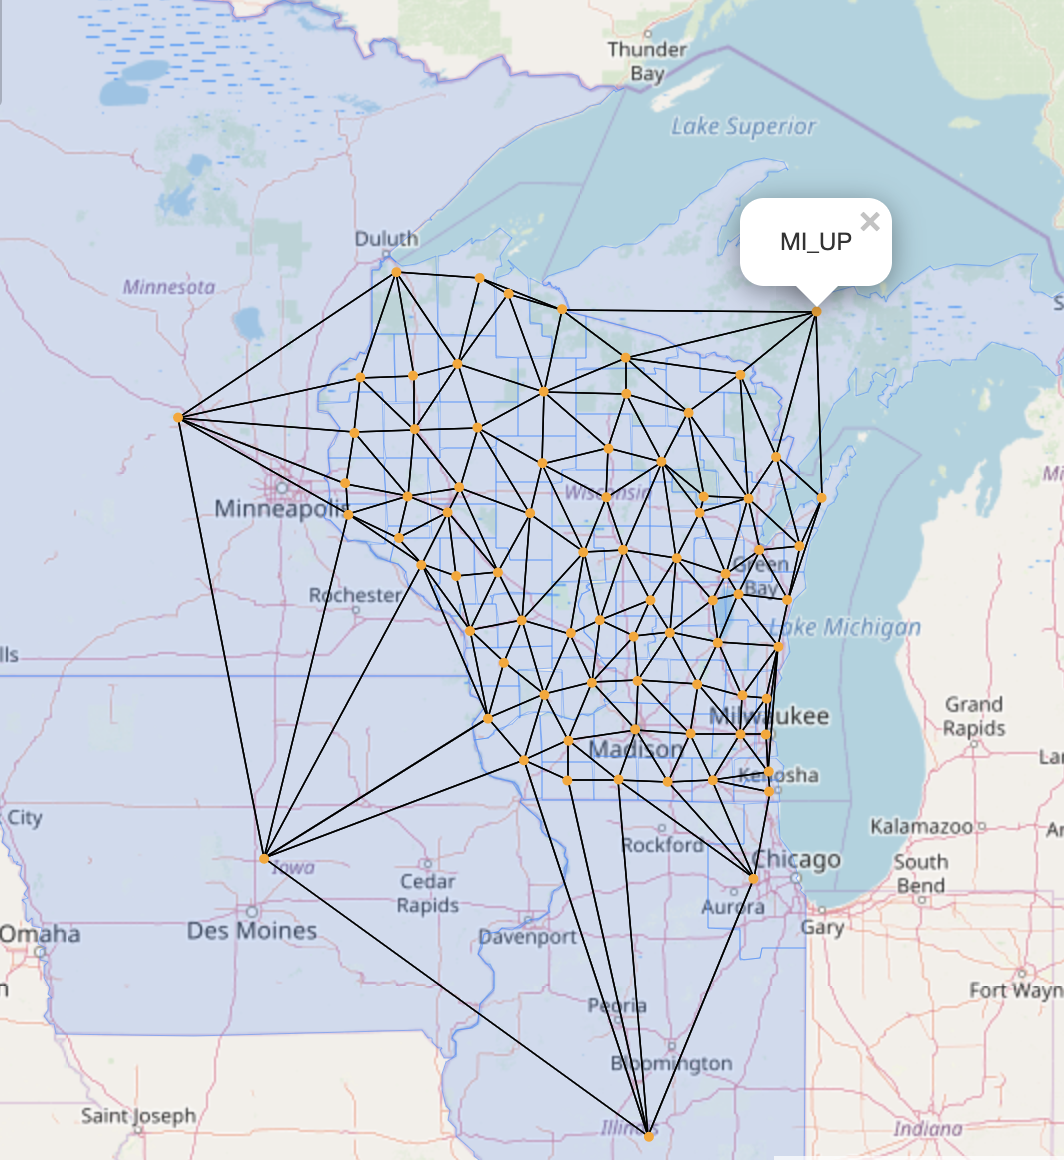
\includegraphics[width=0.25\textwidth]{includes/data_network_no_browser_w_popup.png}
%
% an example load duration curve and the piecewise constant fit that WEREWOLF uses
  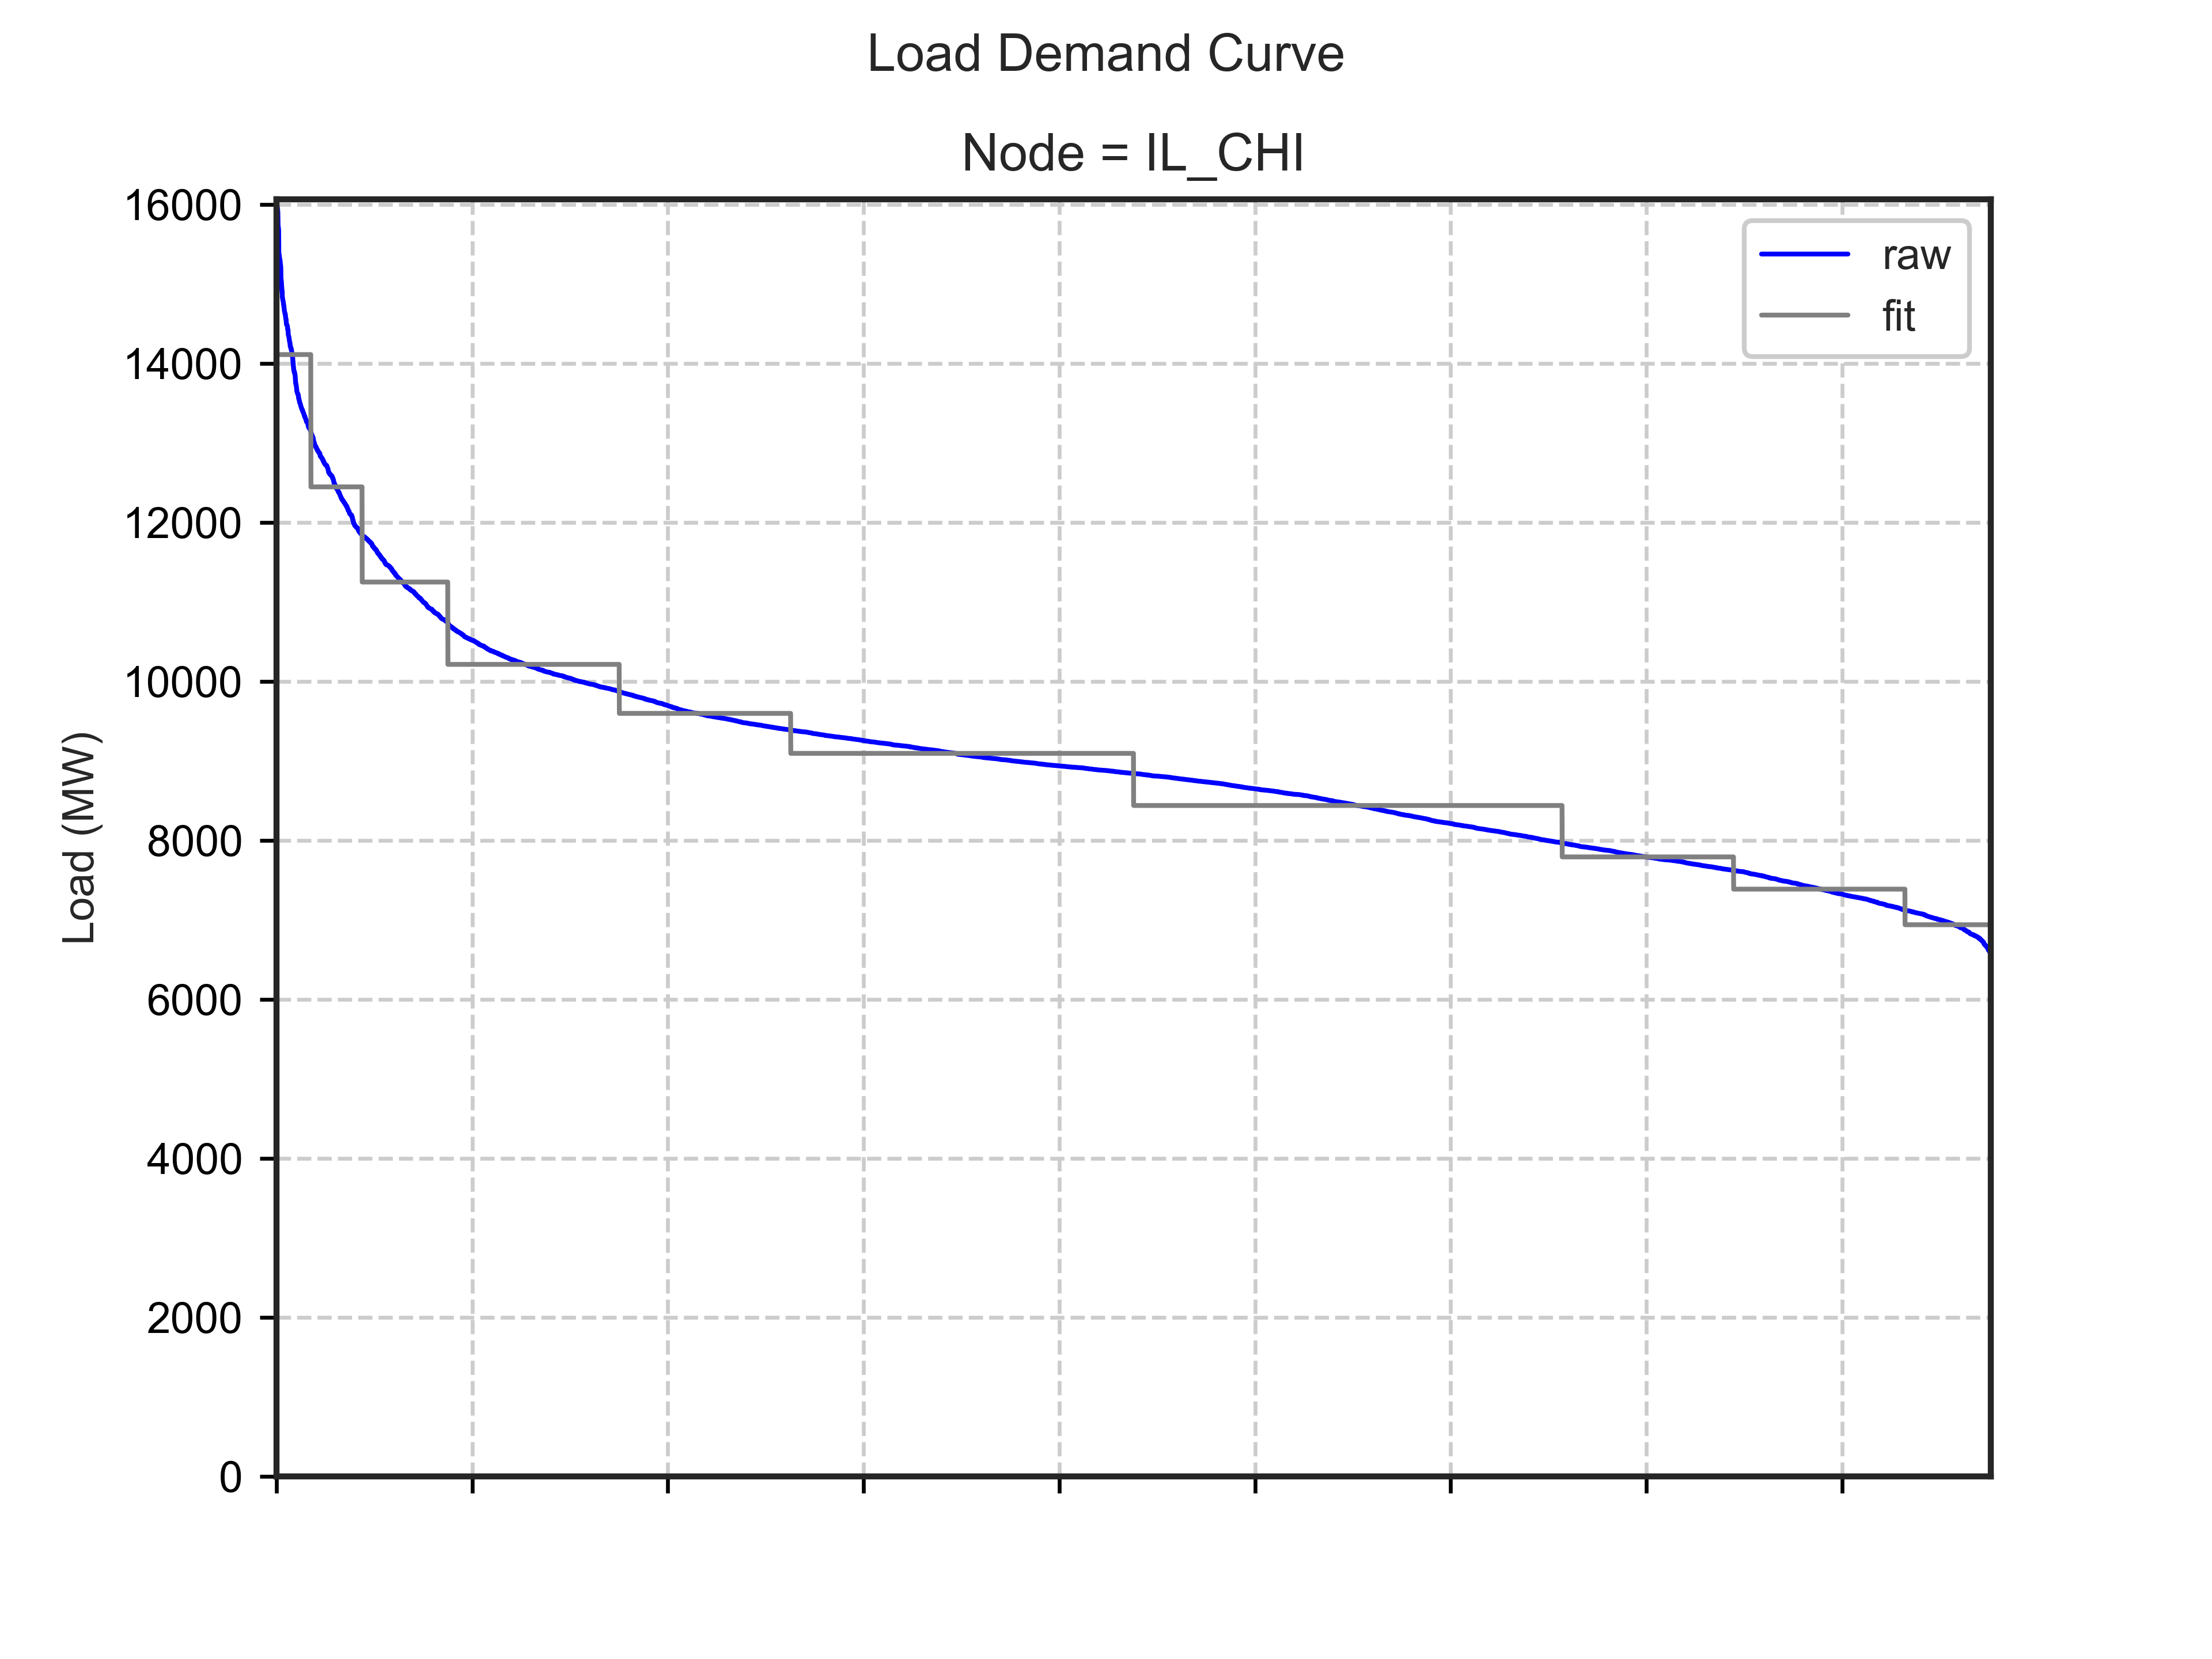
\includegraphics[width=0.45\textwidth]{includes/LDC_node_IL_CHI.png}

\end{frame}


% THIS SLIDE SHOWS RESULTS FROM RUNS THAT DID NOT ALLOW SHUTDOWNS
\begin{frame}
  \frametitle{Carbon reductions (increasing or flat imports)}

\begin{itemize}
  \item Demand in 2030 is a data input, what generation portfolio
    needed for this new demand under increasing carbon reduction requirement
  \item Imports, capacity mix (no plant shutdowns),  generation
\end{itemize}

% the story here is that unrestricted imports allows WI to get to deep carbon reductions with the caveat that there might be deficiencies with the transmission network model description

  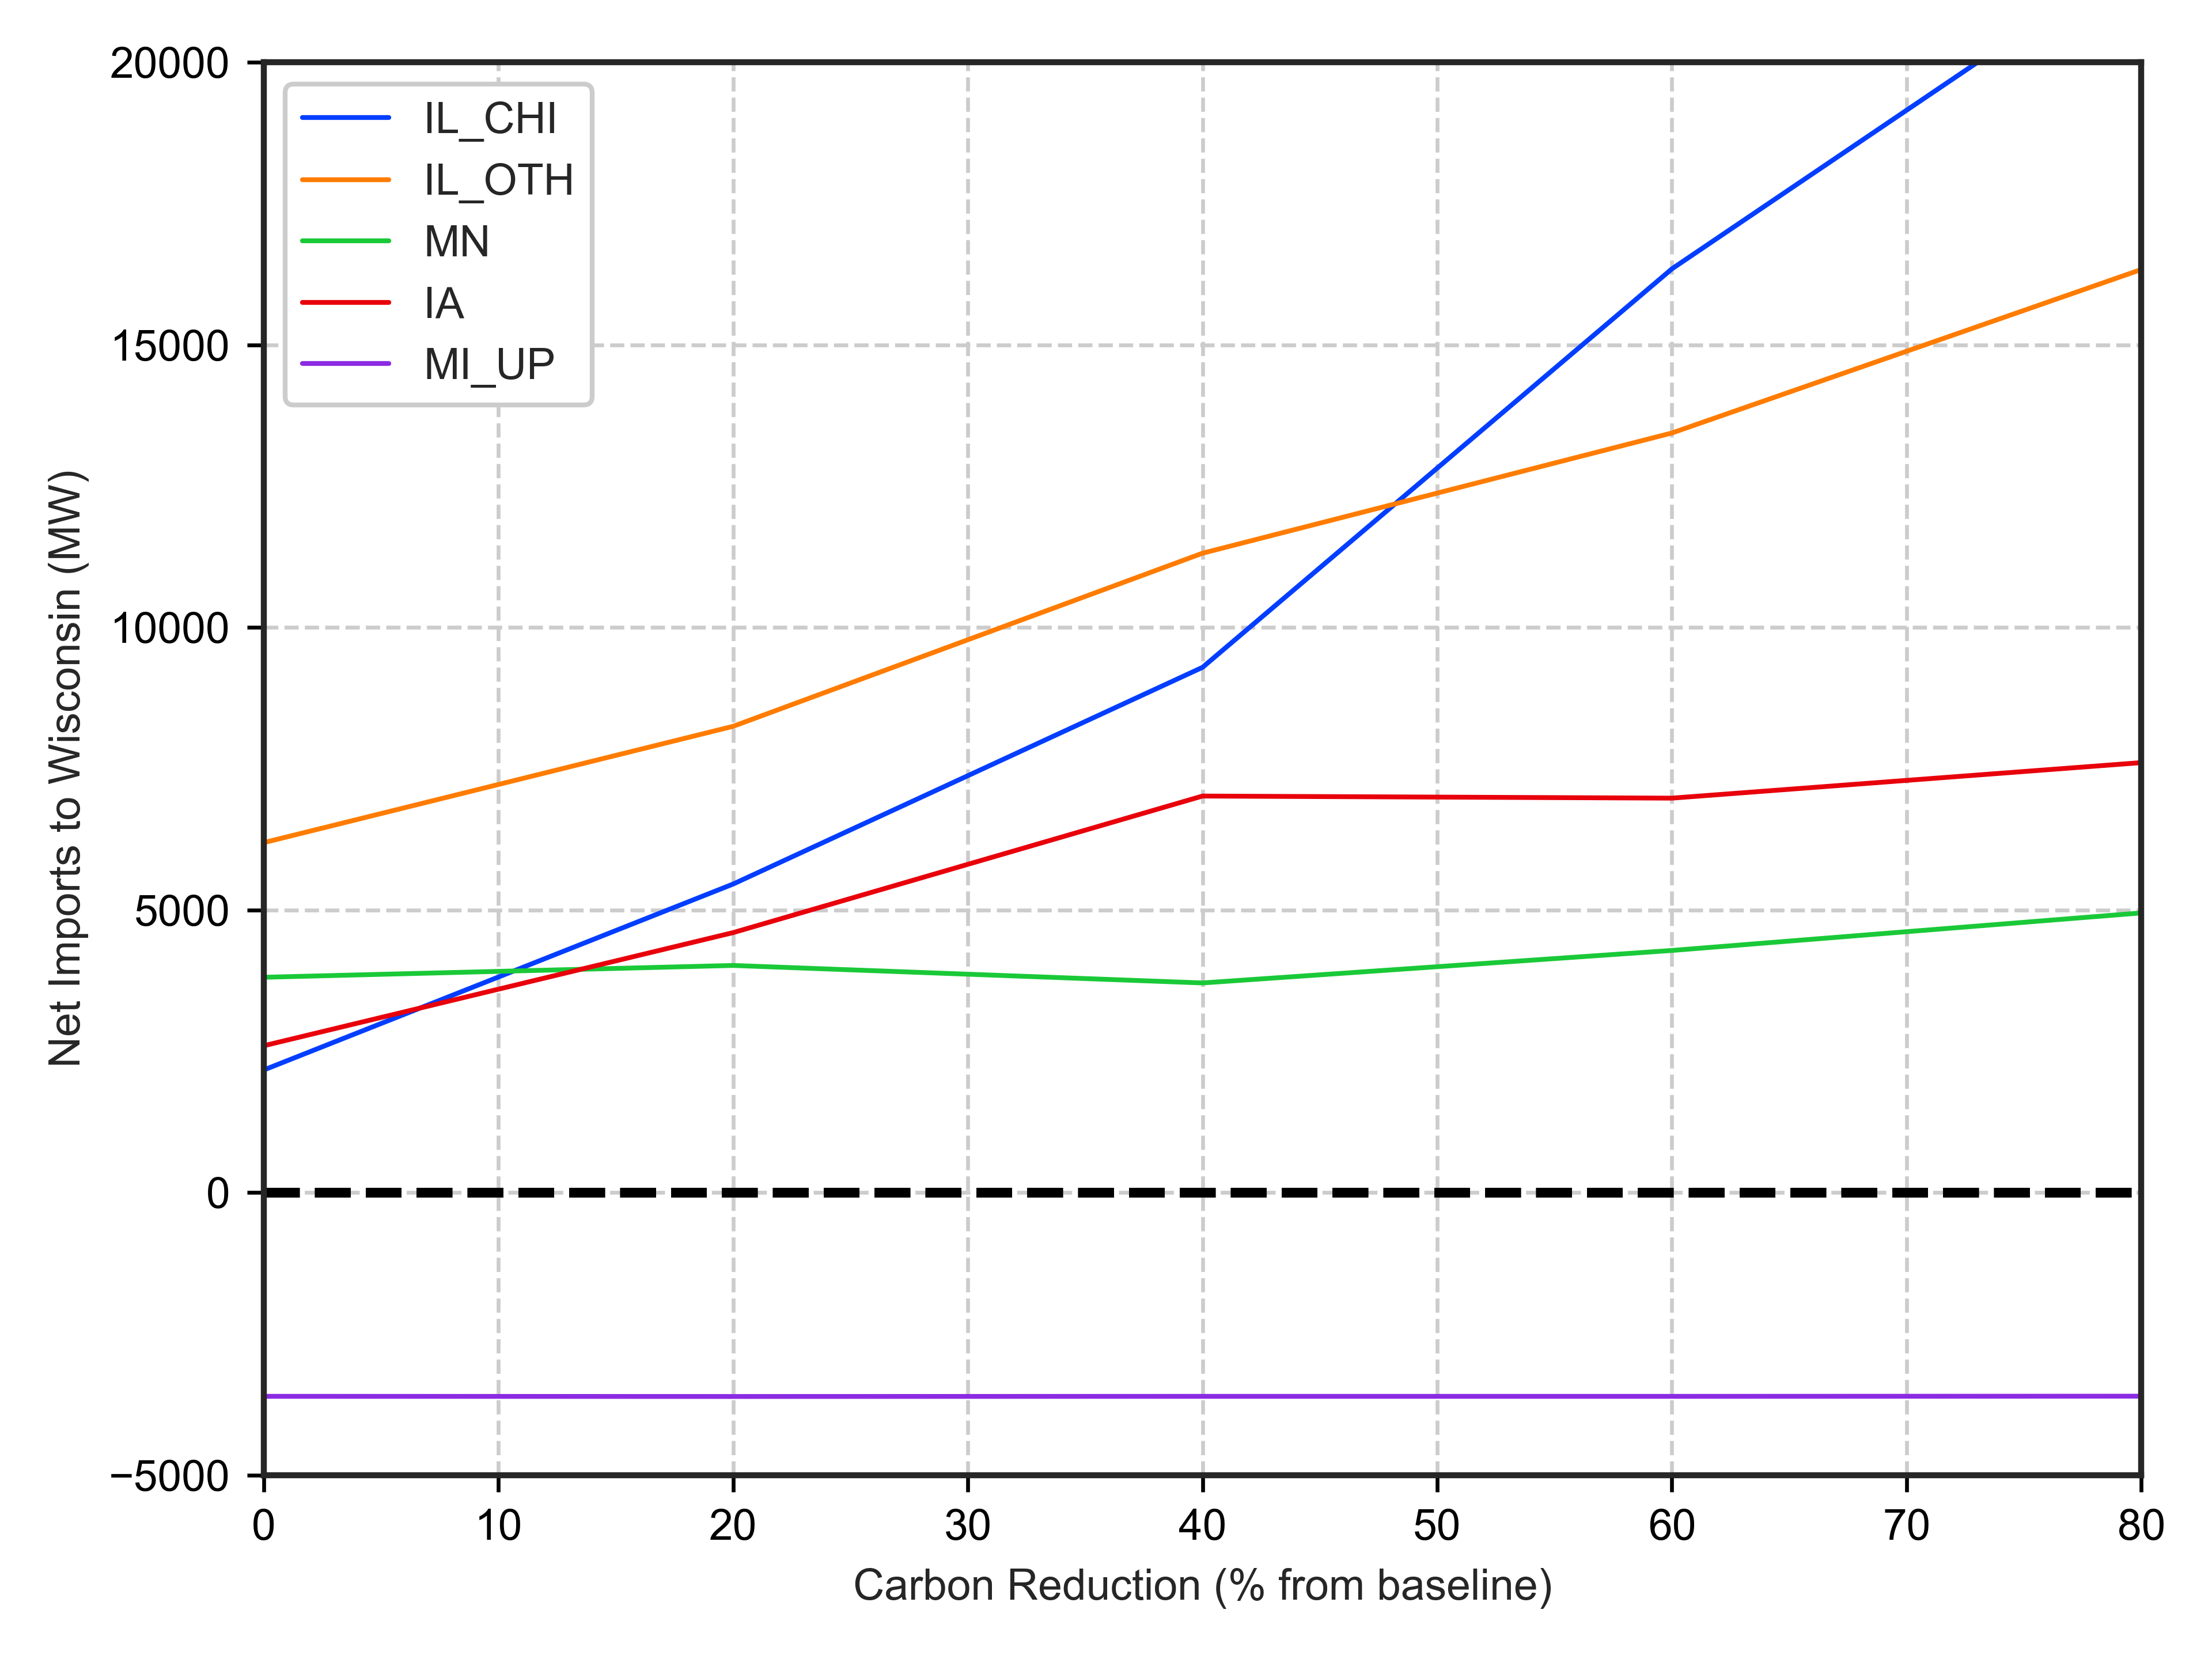
\includegraphics[width=0.32\textwidth]{includes/leakage_no_shutdowns_agg_exim.png}
  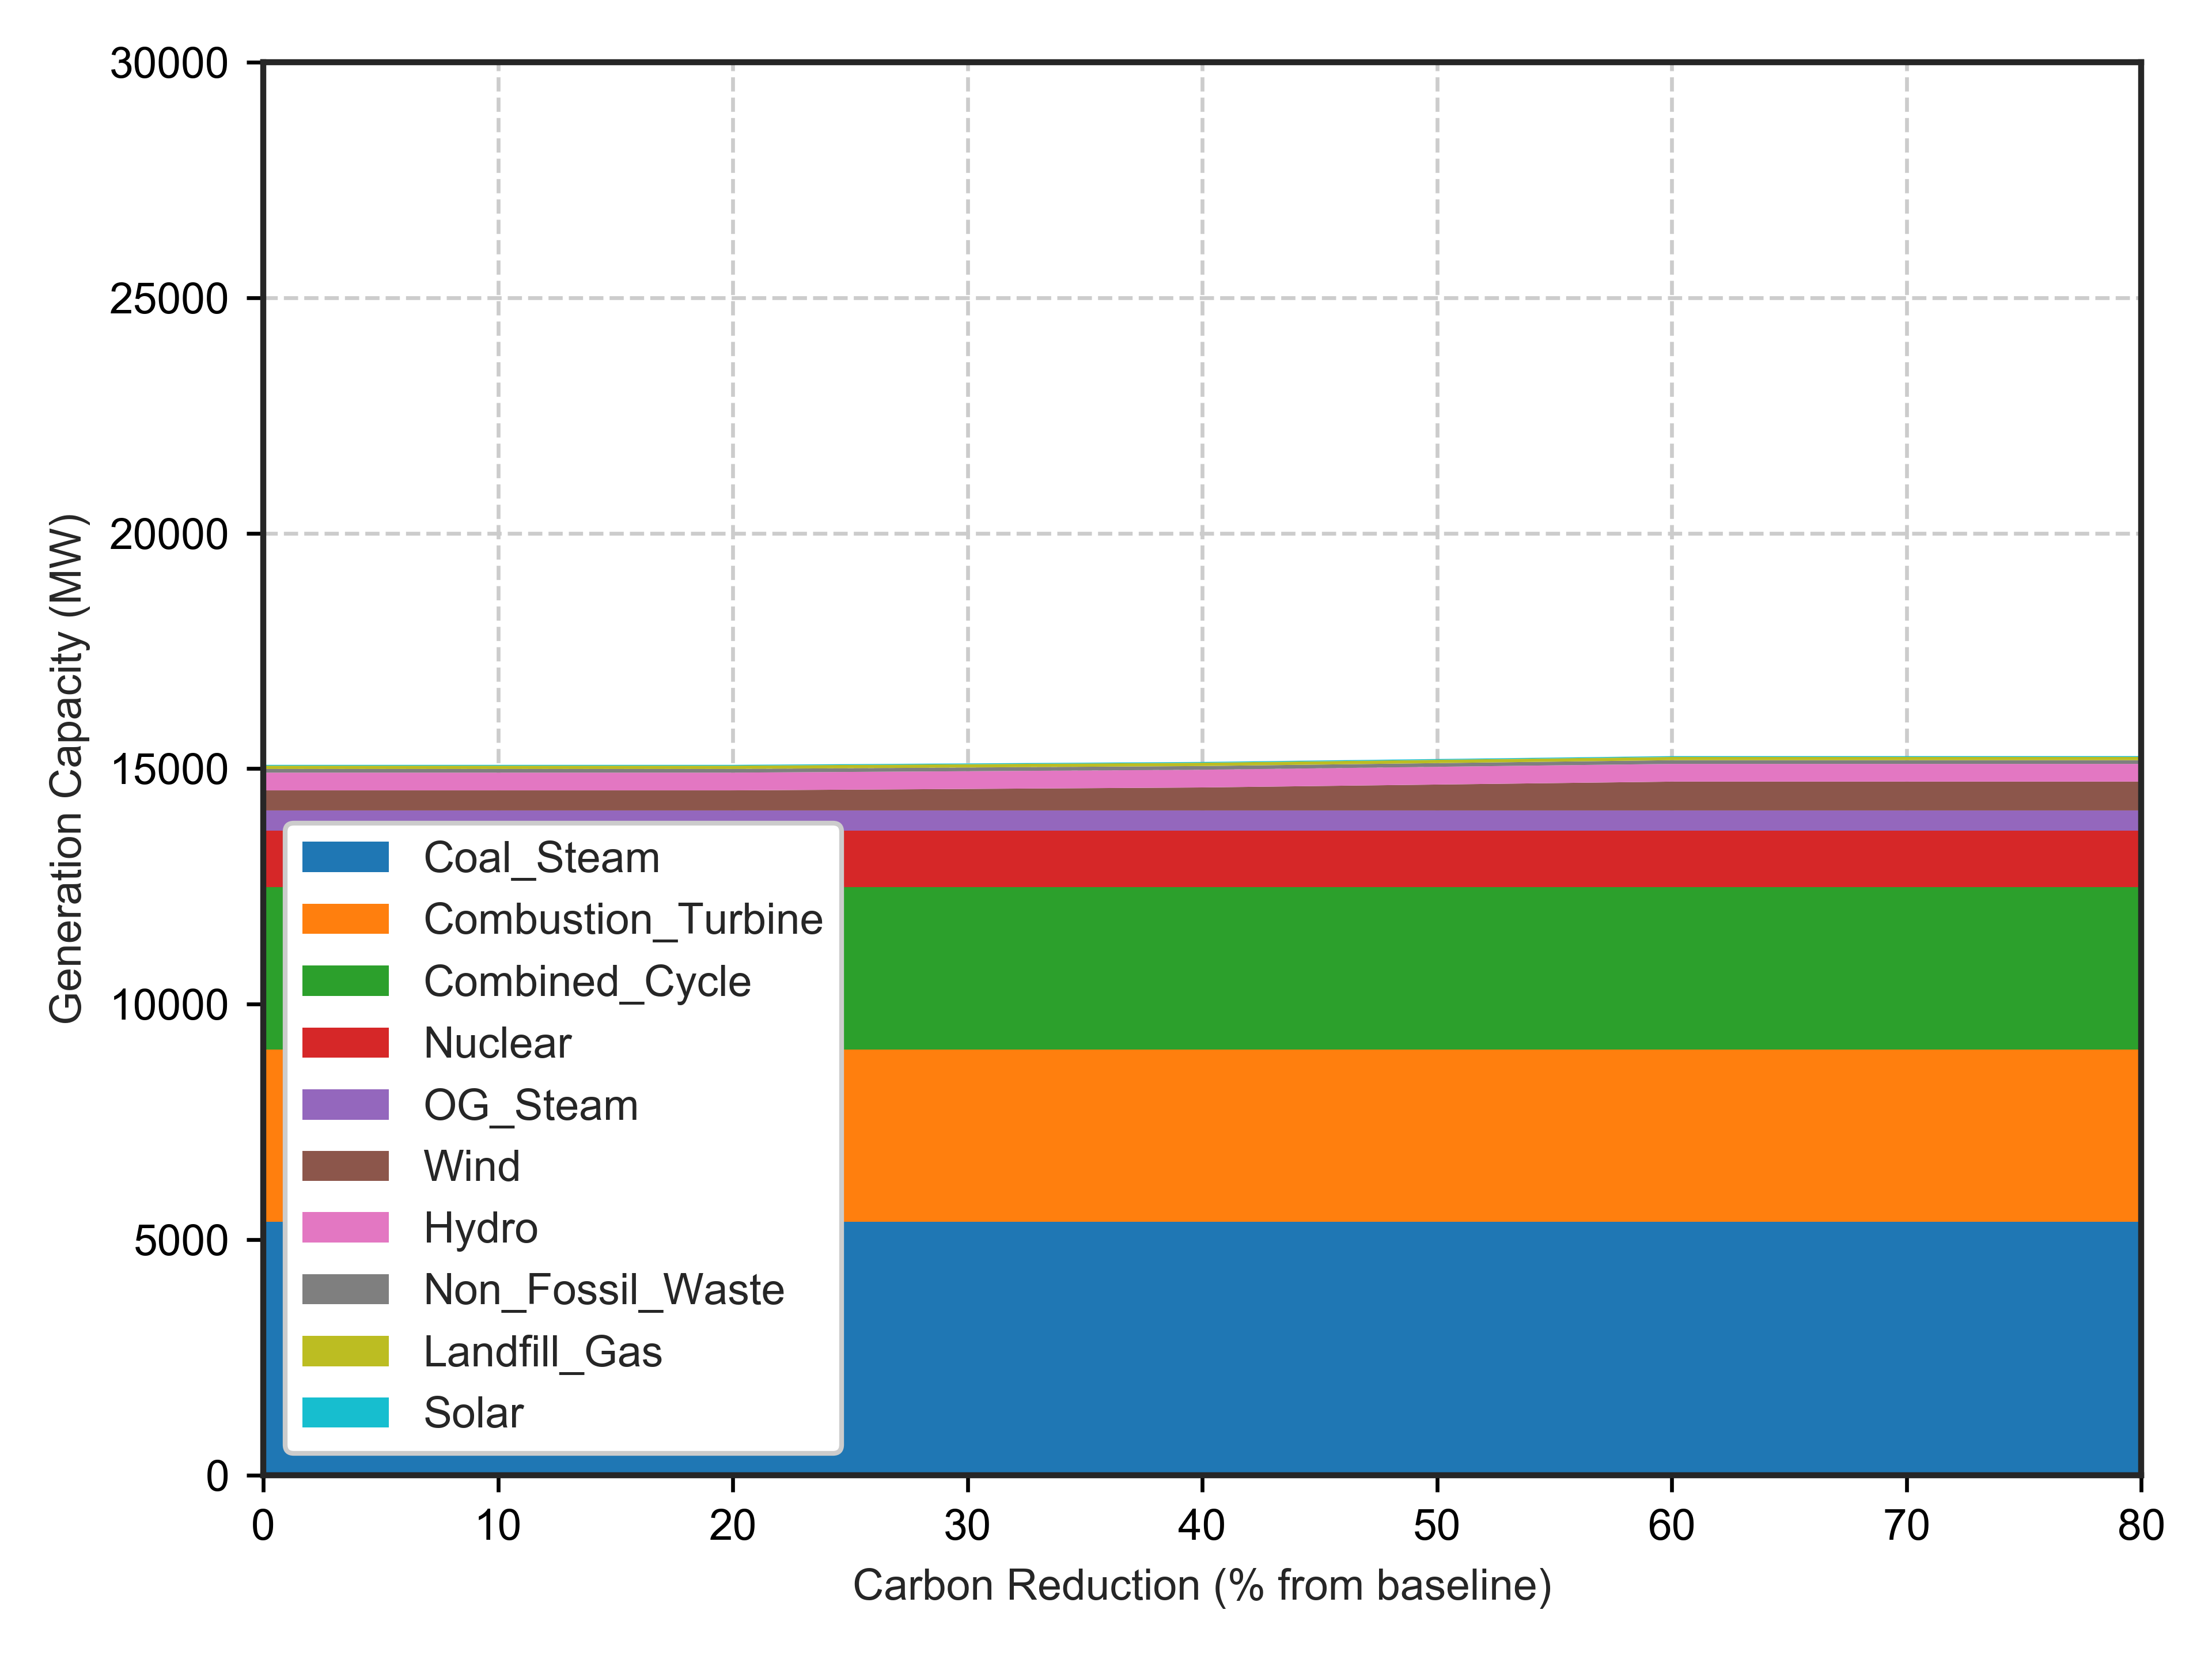
\includegraphics[width=0.32\textwidth]{includes/leakage_no_shutdowns_agg_capacity_cntlreg.png}
% this is the actual generation for the carbon leak scenario (WI only)
  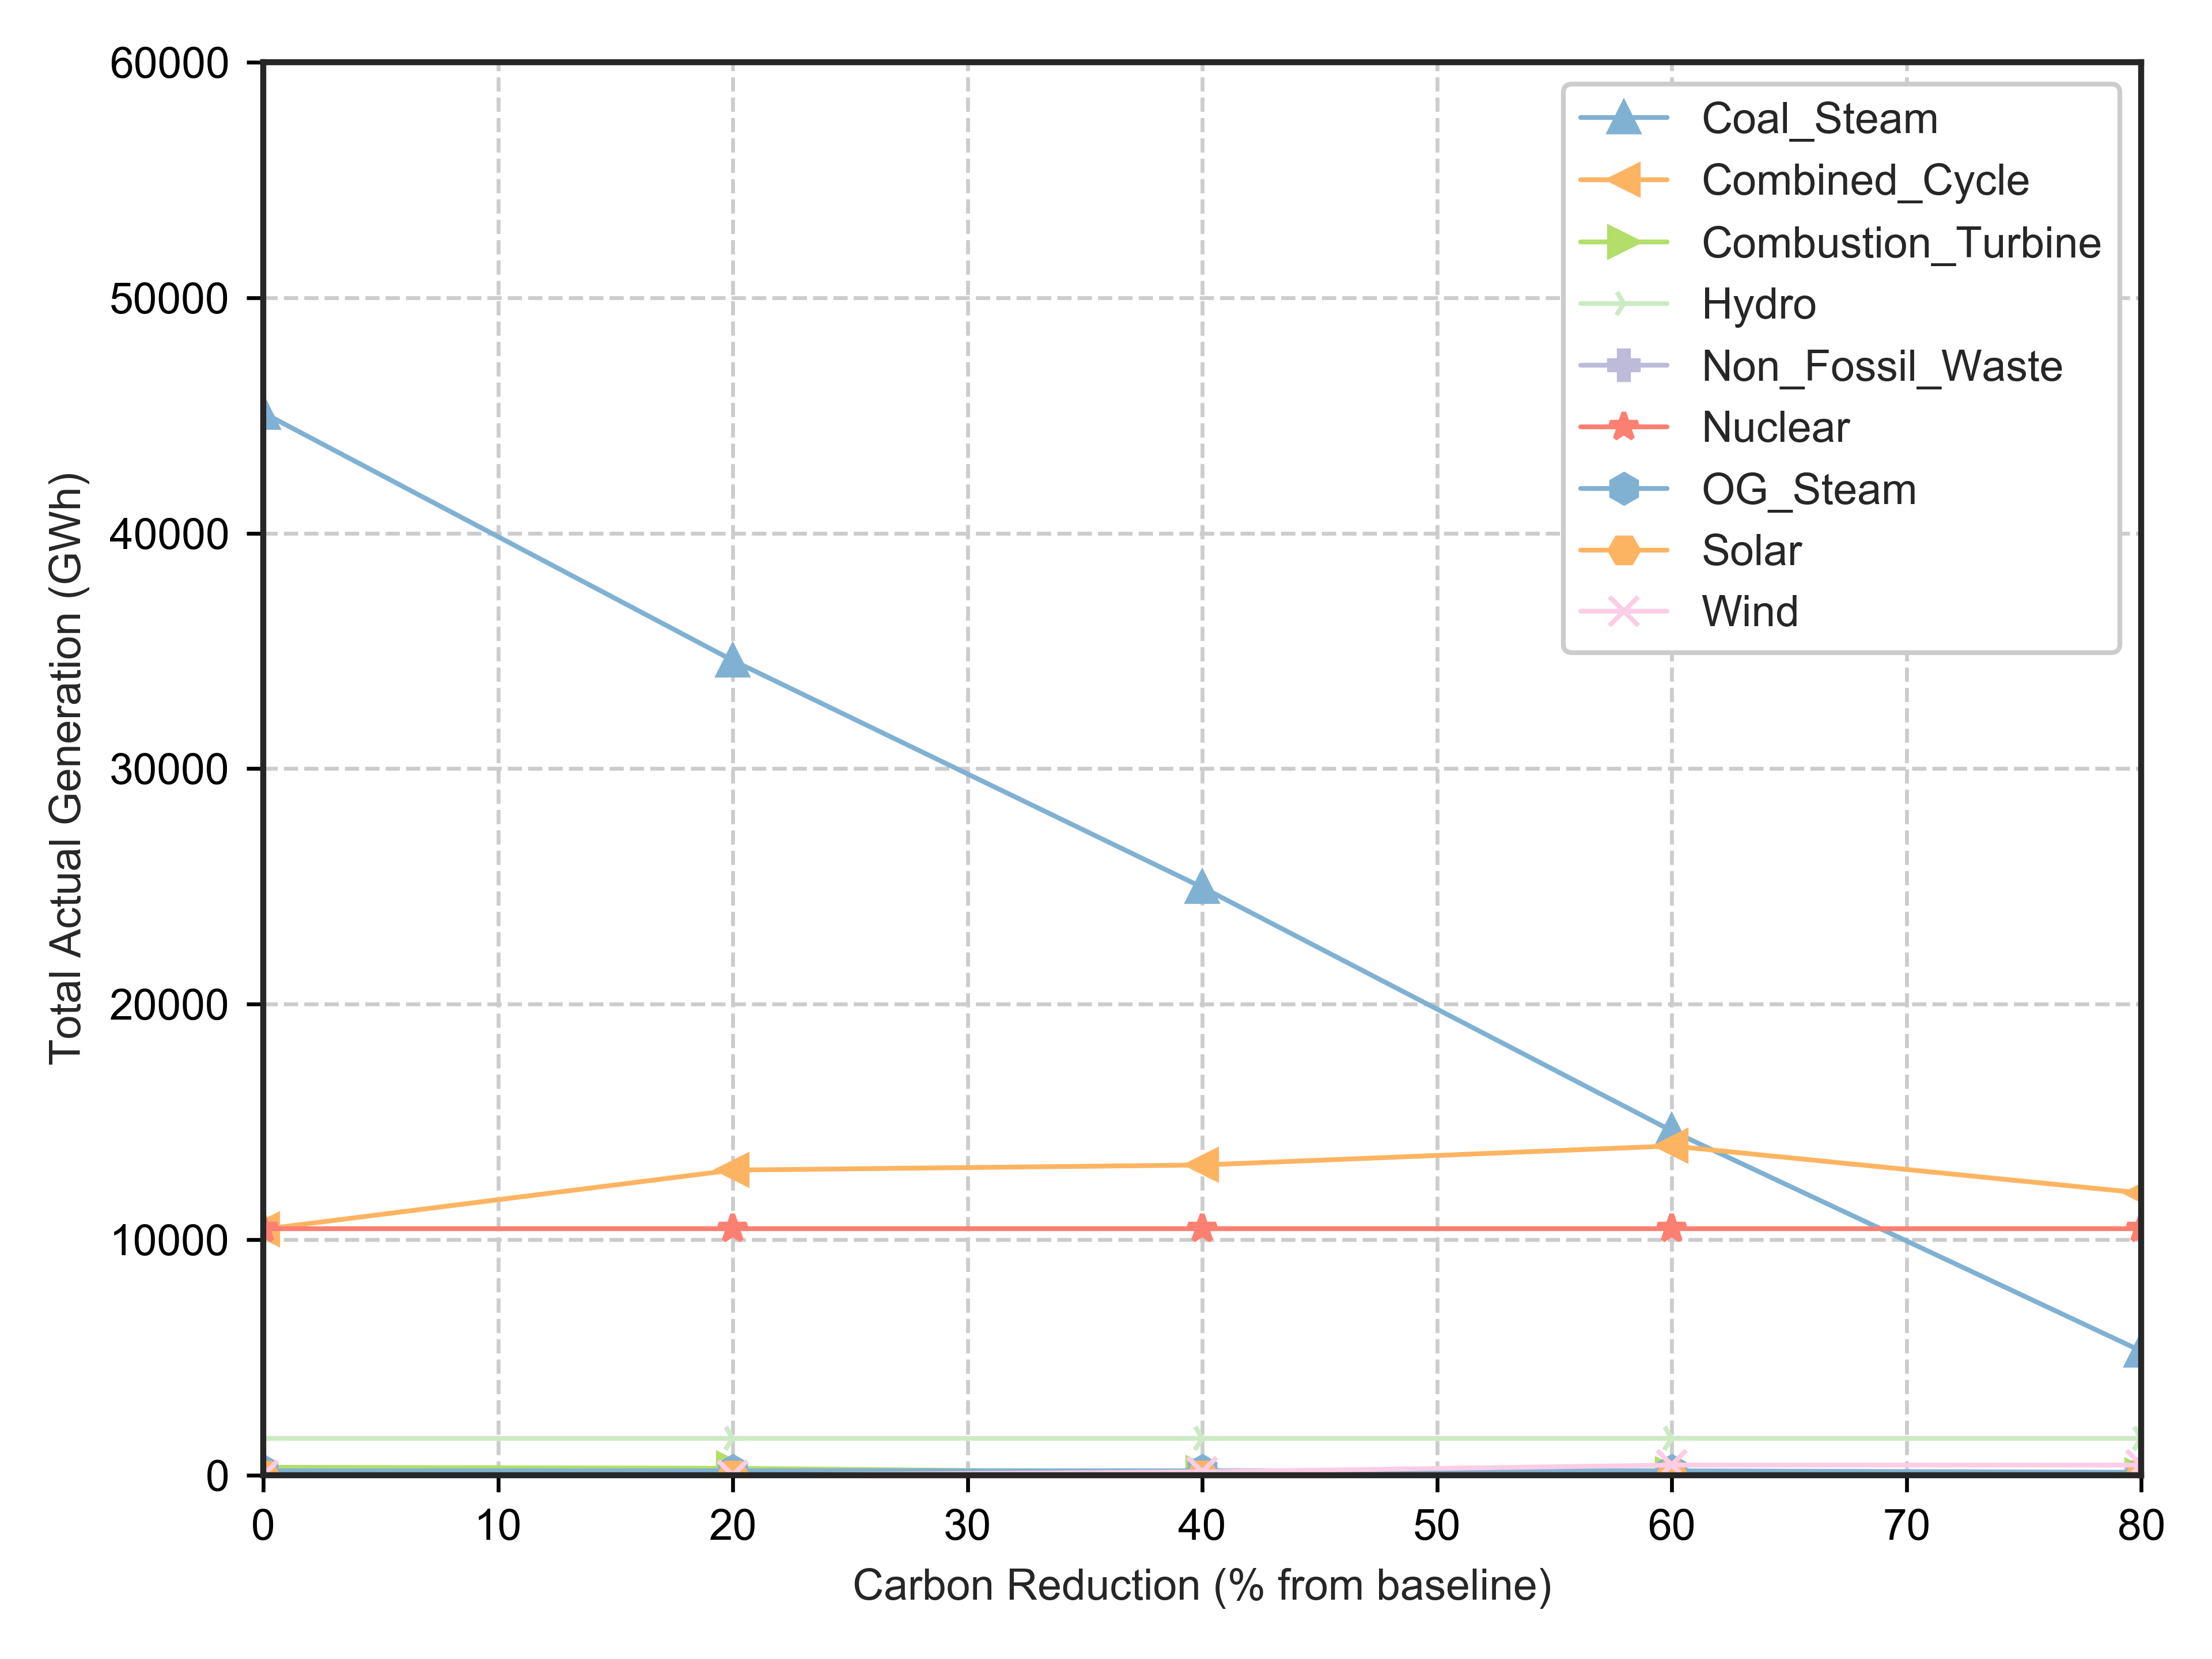
\includegraphics[width=0.32\textwidth]{includes/leakage_no_shutdowns_agg_generation_cntlreg.png}

  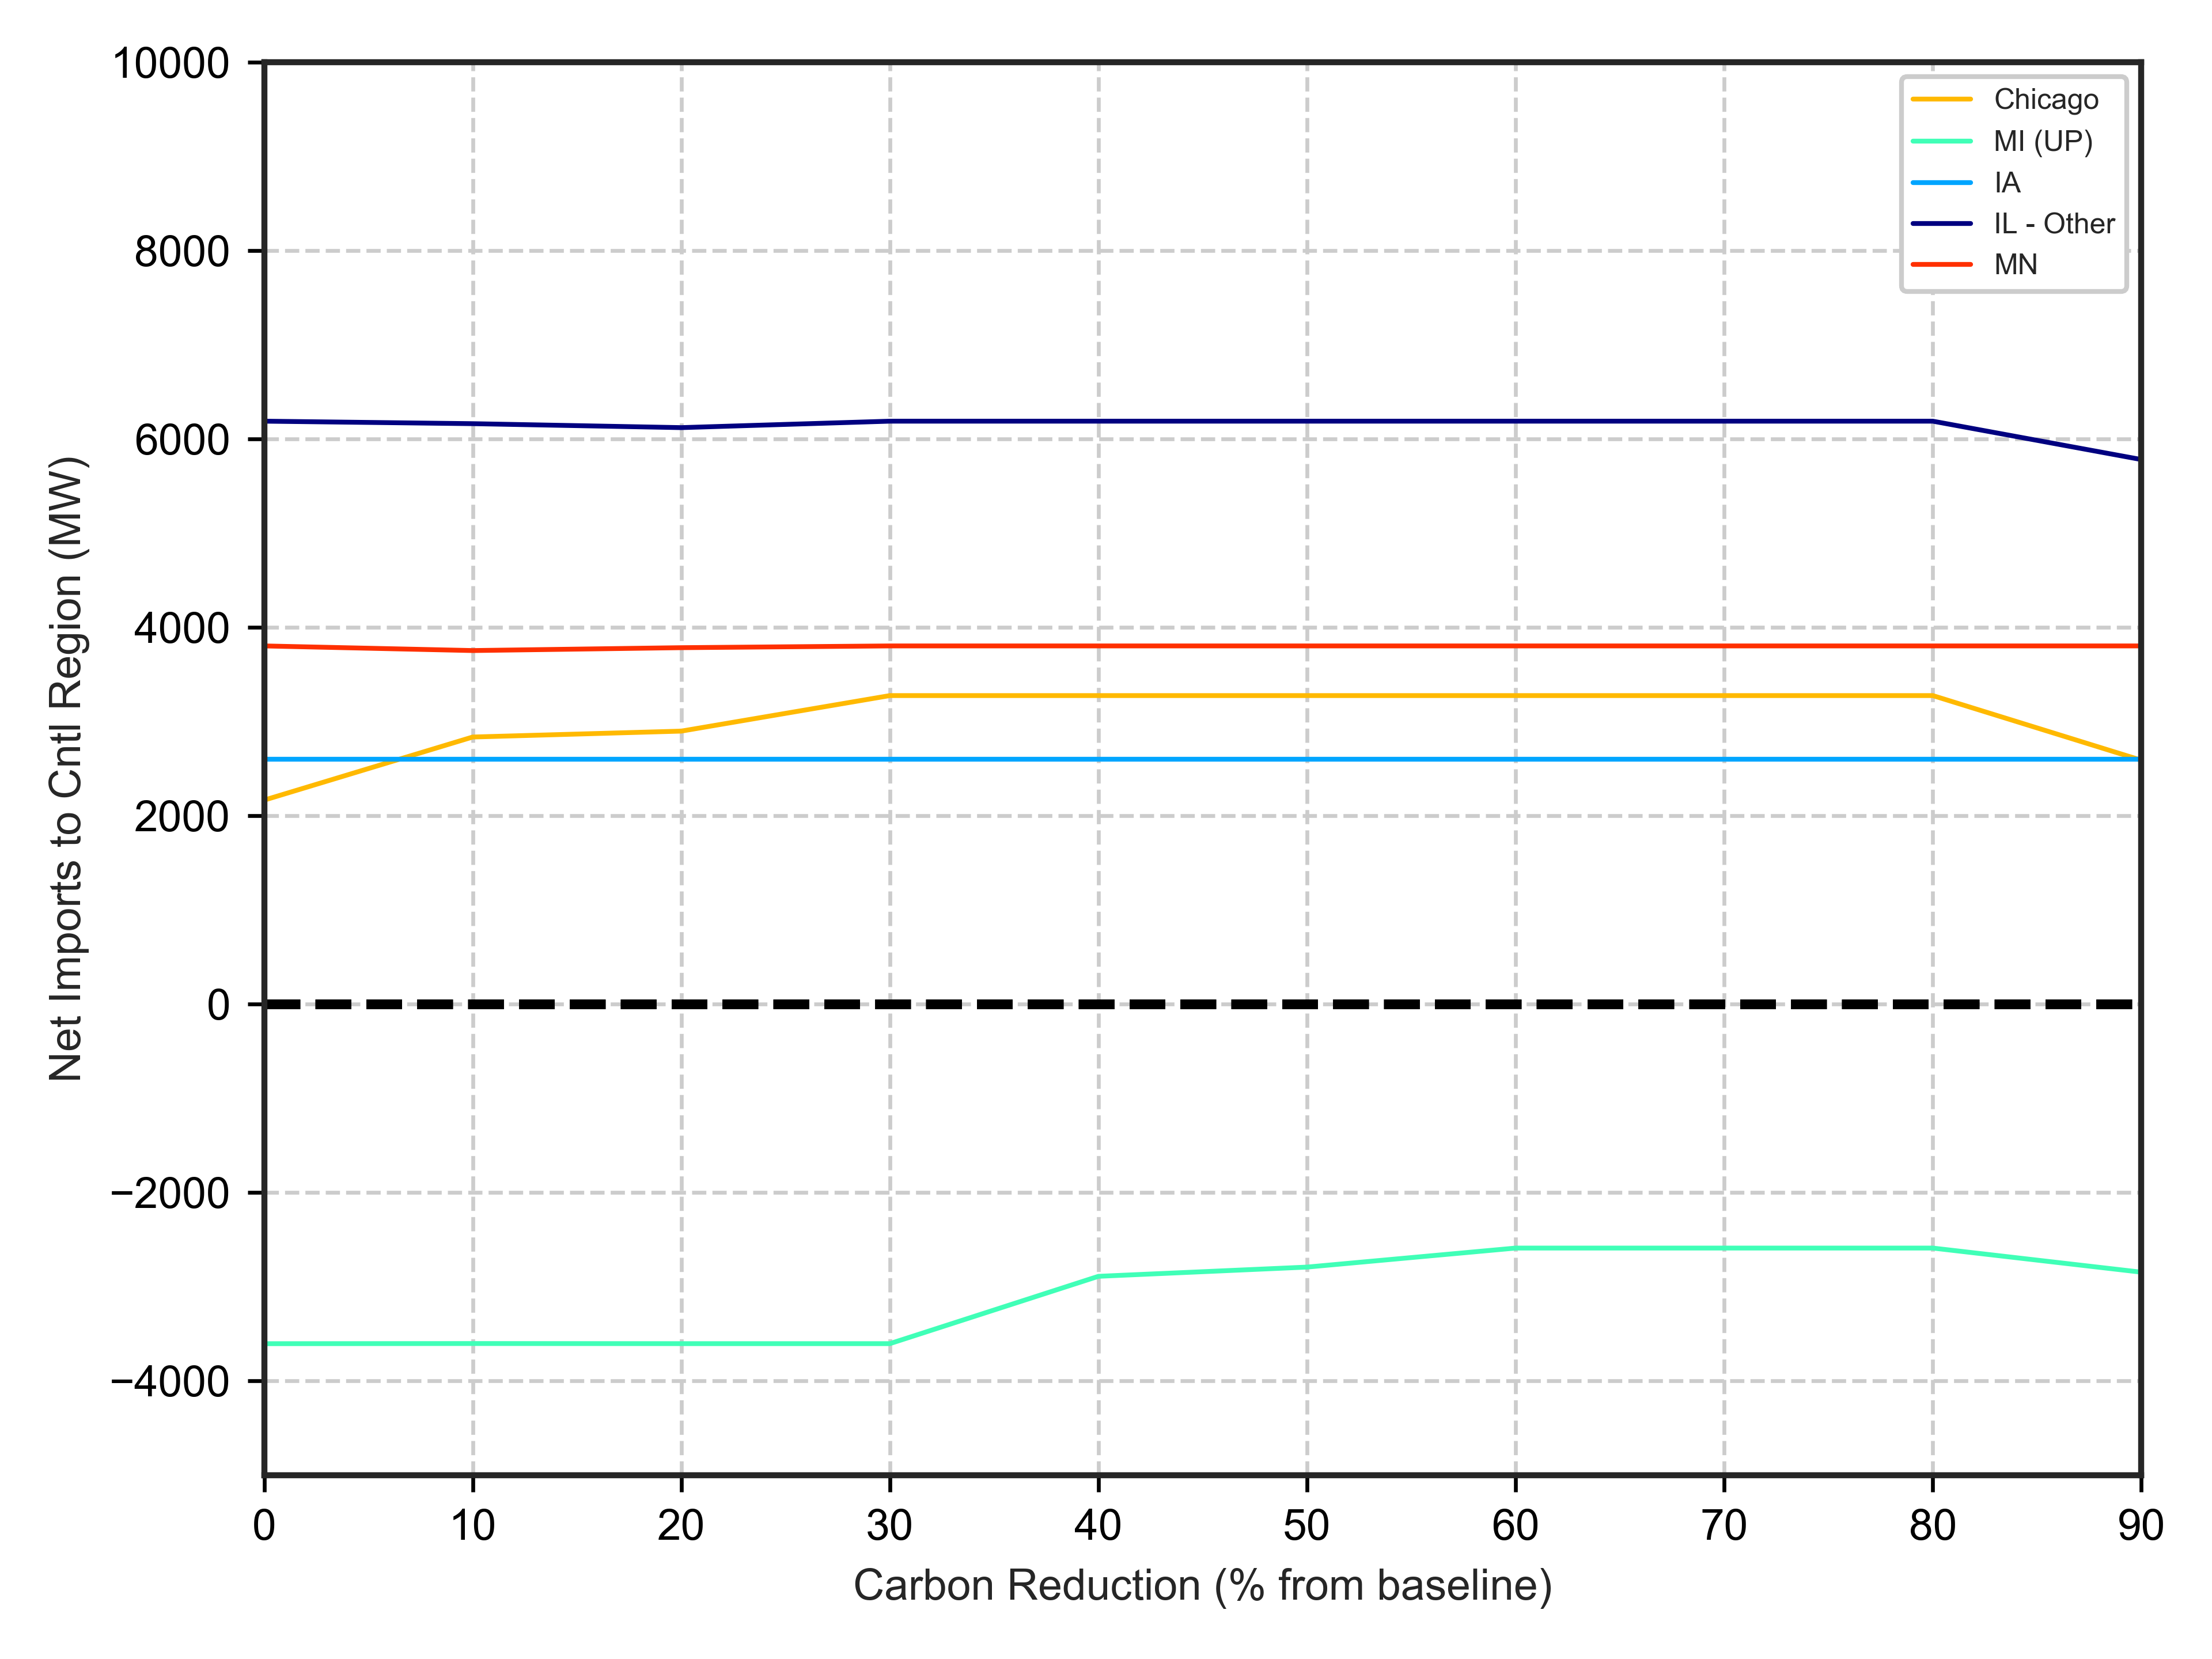
\includegraphics[width=0.32\textwidth]{includes/no_leakage_no_shutdowns_agg_exim.png}
  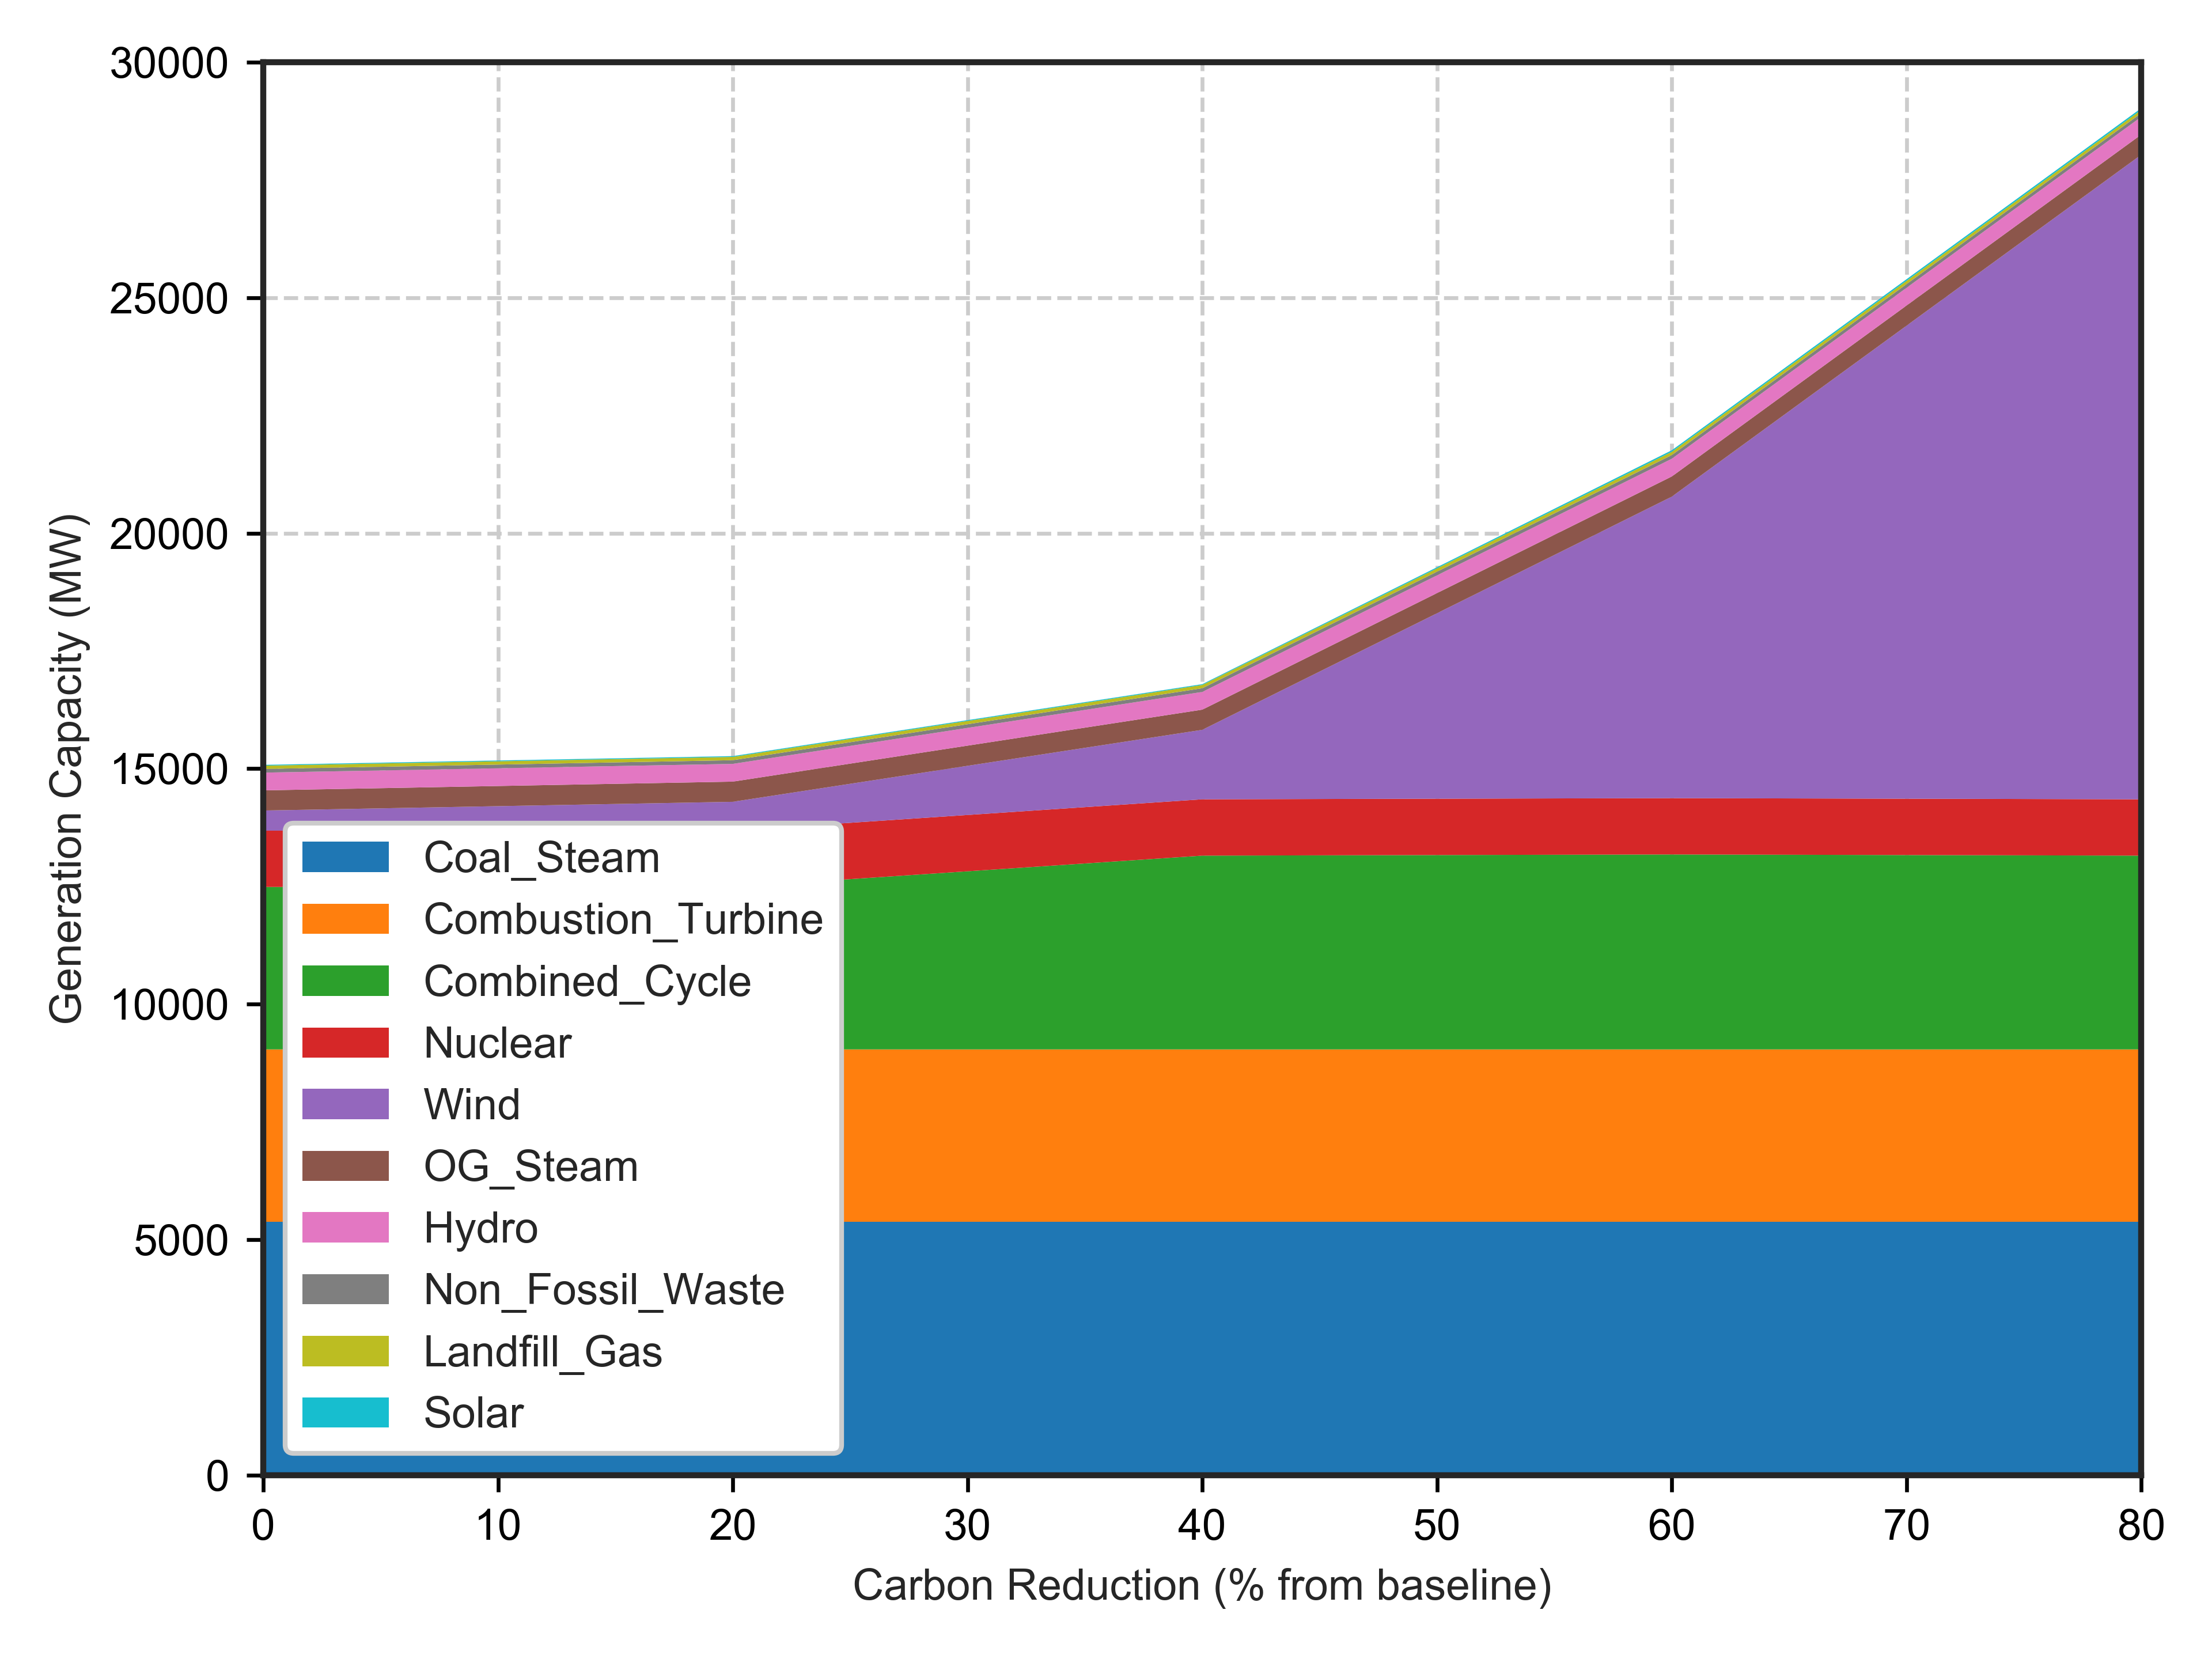
\includegraphics[width=0.32\textwidth]{includes/no_leakage_no_shutdowns_agg_capacity_cntlreg.png}
% this is the actual generation for the NO carbon leak scenario (WI only)
  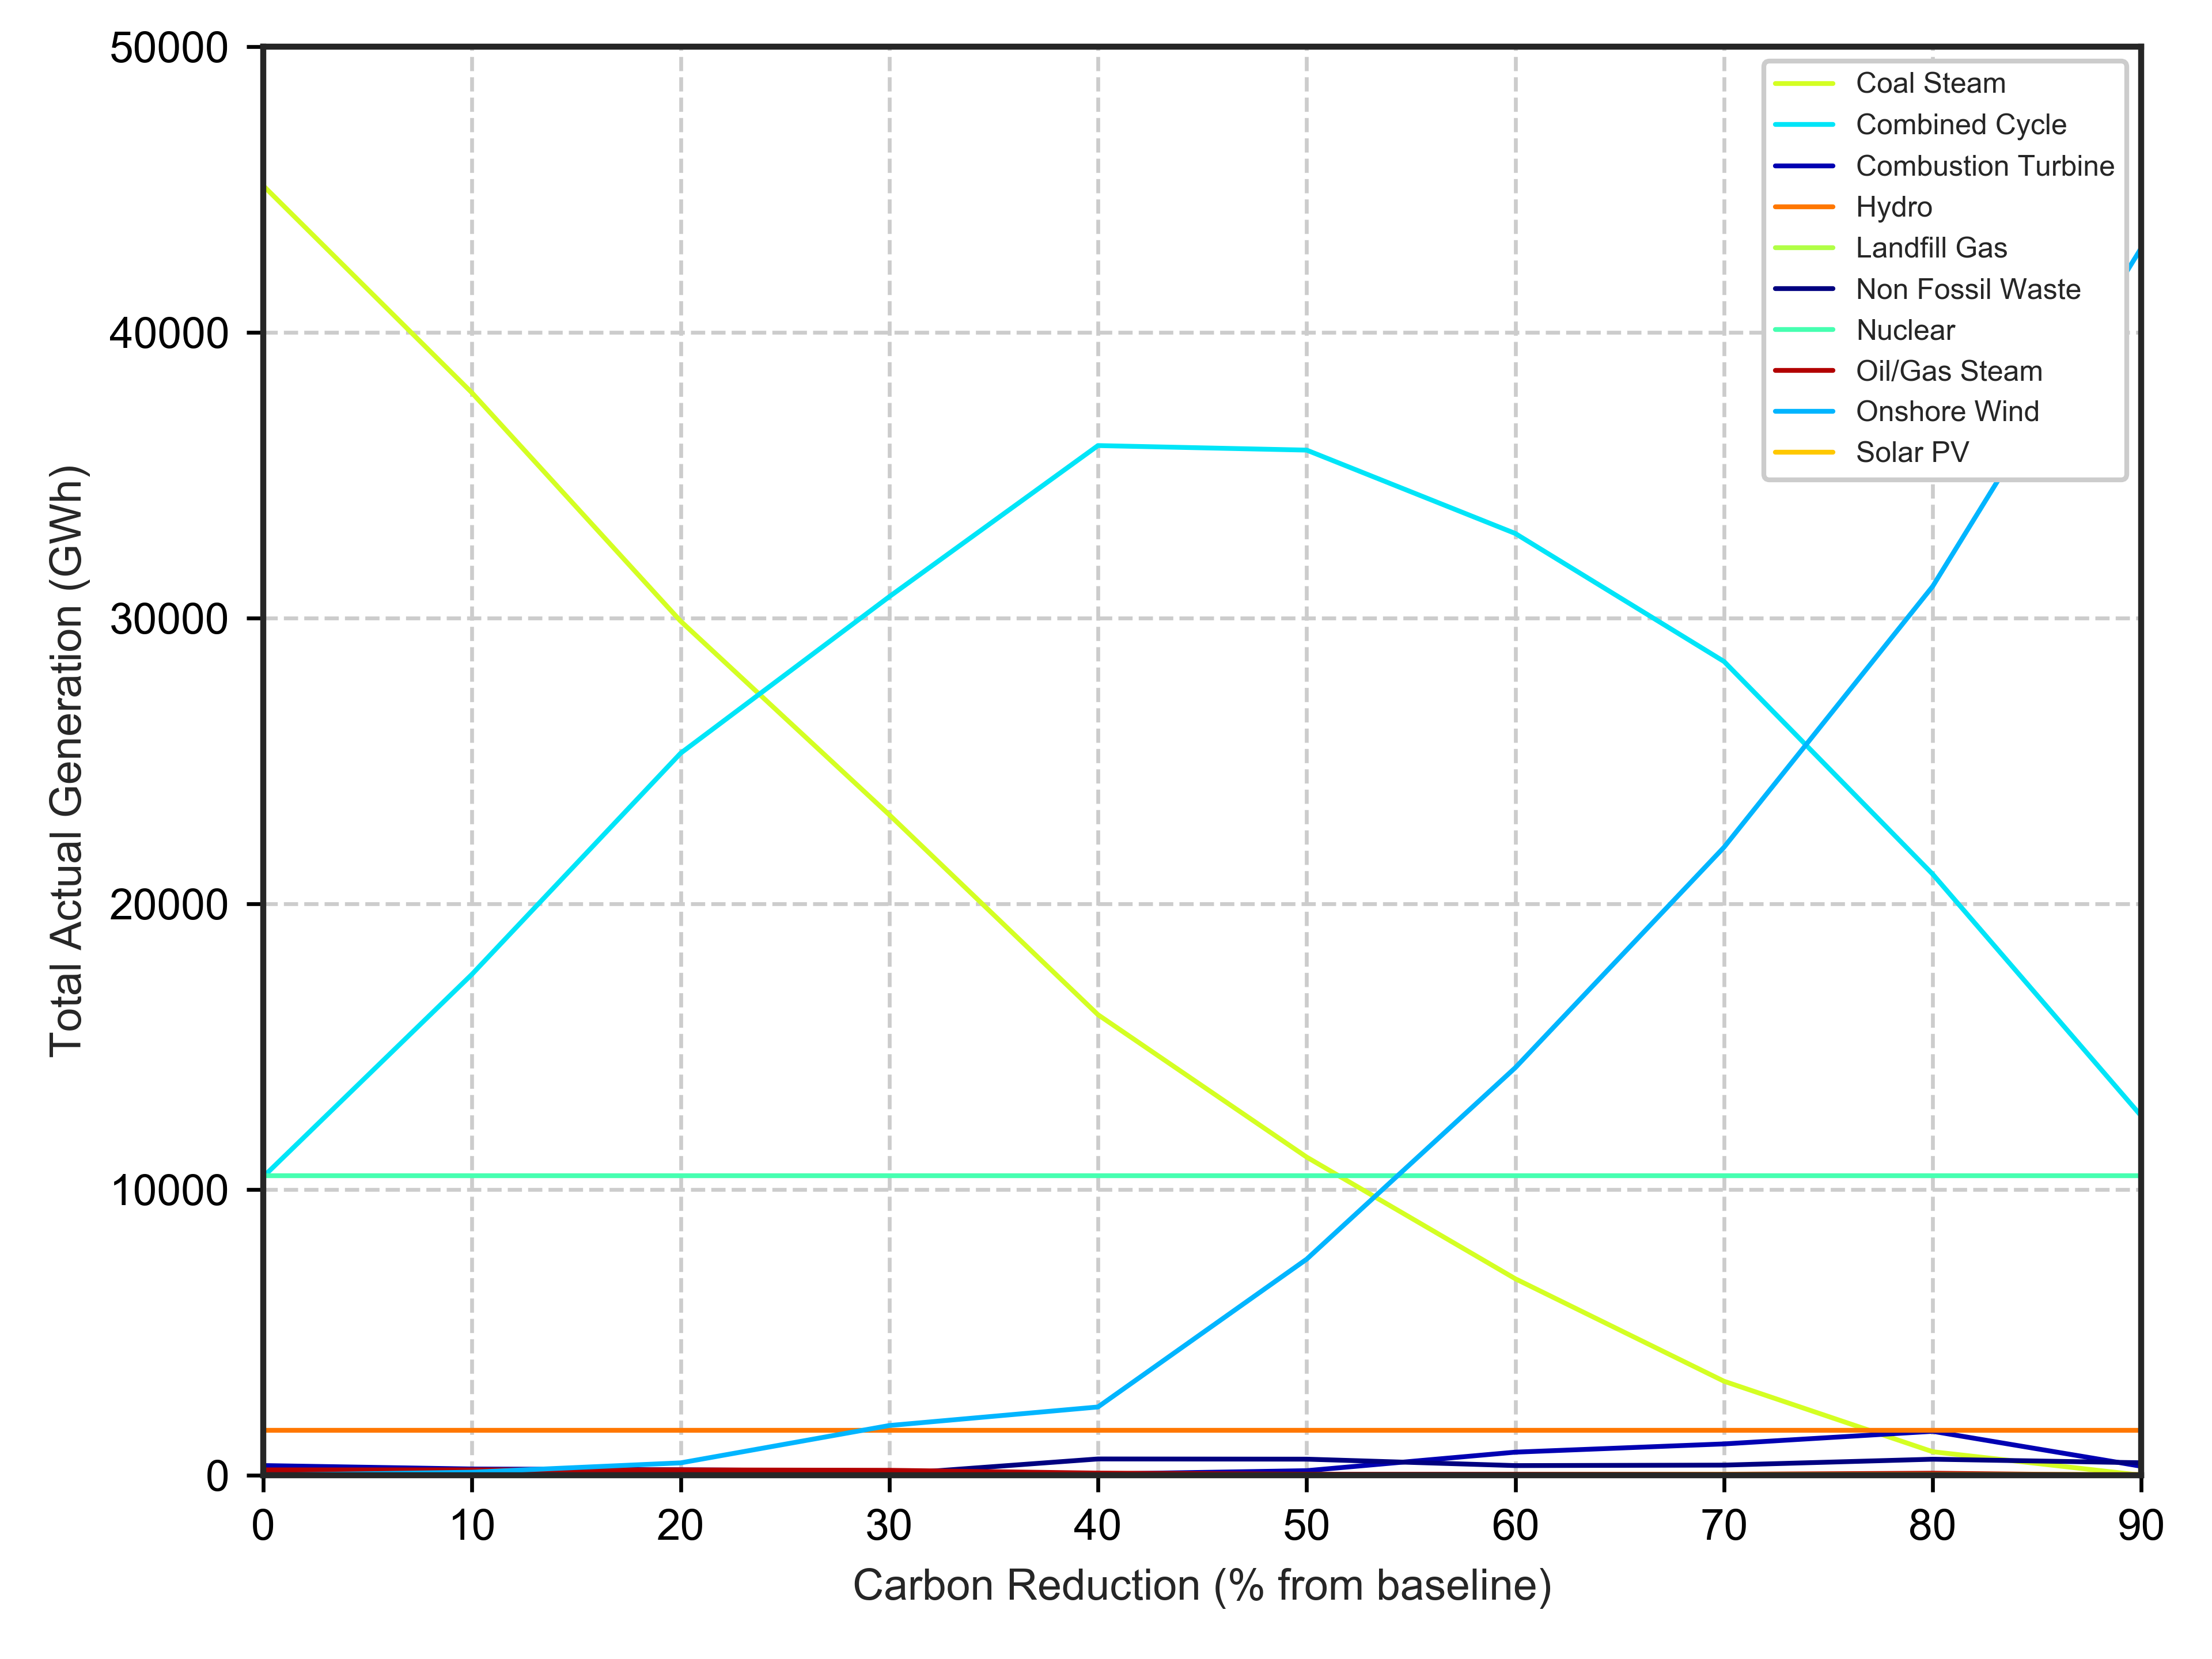
\includegraphics[width=0.32\textwidth]{includes/no_leakage_no_shutdowns_agg_generation_cntlreg.png}

\end{frame}


% THIS SLIDE SHOWS RESULTS FROM RUNS THAT DID ALLOW SHUTDOWNS
\begin{frame}
  \frametitle{Carbon leakage (increasing or flat imports) -- Shutdowns Allowed}
\begin{itemize}
  \item Demand in 2030 is a data input, but what is the right investment now for this new demand?
  \item What is the right action (shutdown/investment) for this new
    demand + additional policies? 
\end{itemize}

% the story here is that unrestricted imports allows WI to get to deep carbon reductions with the caveat that there might be deficiencies with the transmission network model description
% The other story here is that we we allow shutdowns then nuclear will turn off by 2030 if carbon emissions stay the same.  This generation is replaced with combustion turbine.  Nucelar, while cheap to run once it's built is still very expensive to maintain (I have confidence in these costs, they are from NREL now). If carbon policies are active and strong (>40% reduction) then nuclear has a very important role to play.

  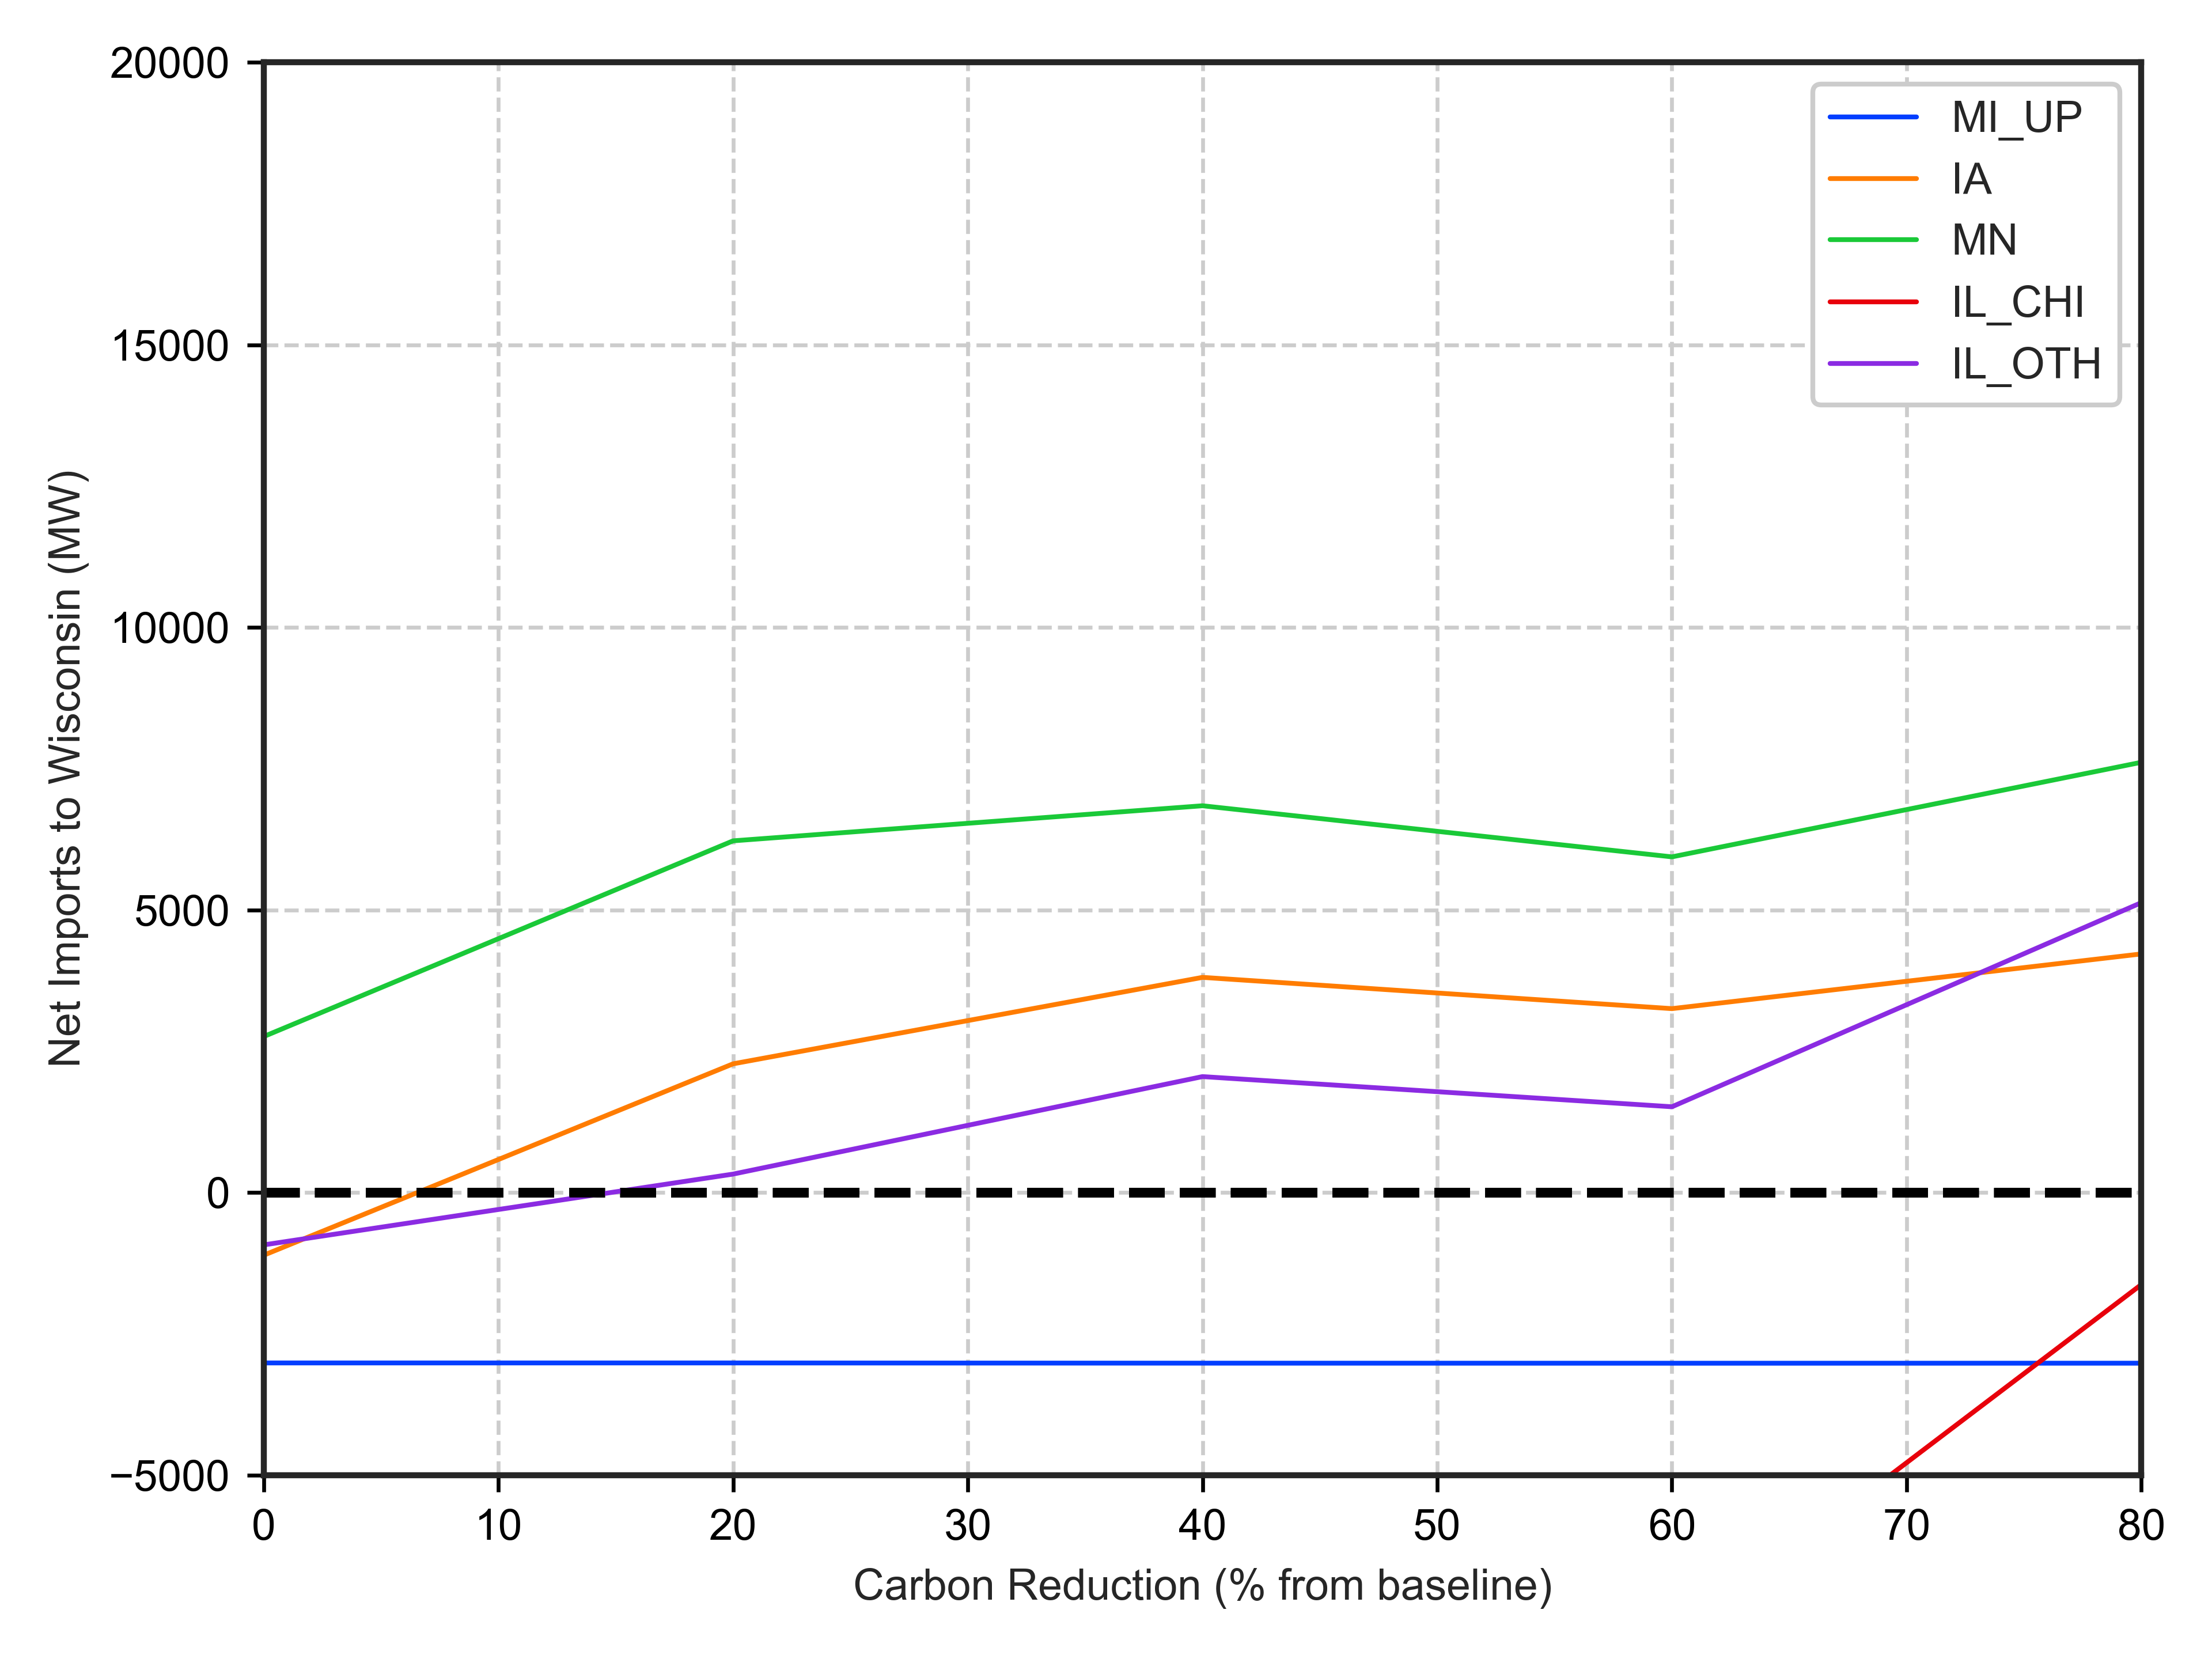
\includegraphics[width=0.32\textwidth]{includes/leakage_shutdowns_agg_exim.png}
  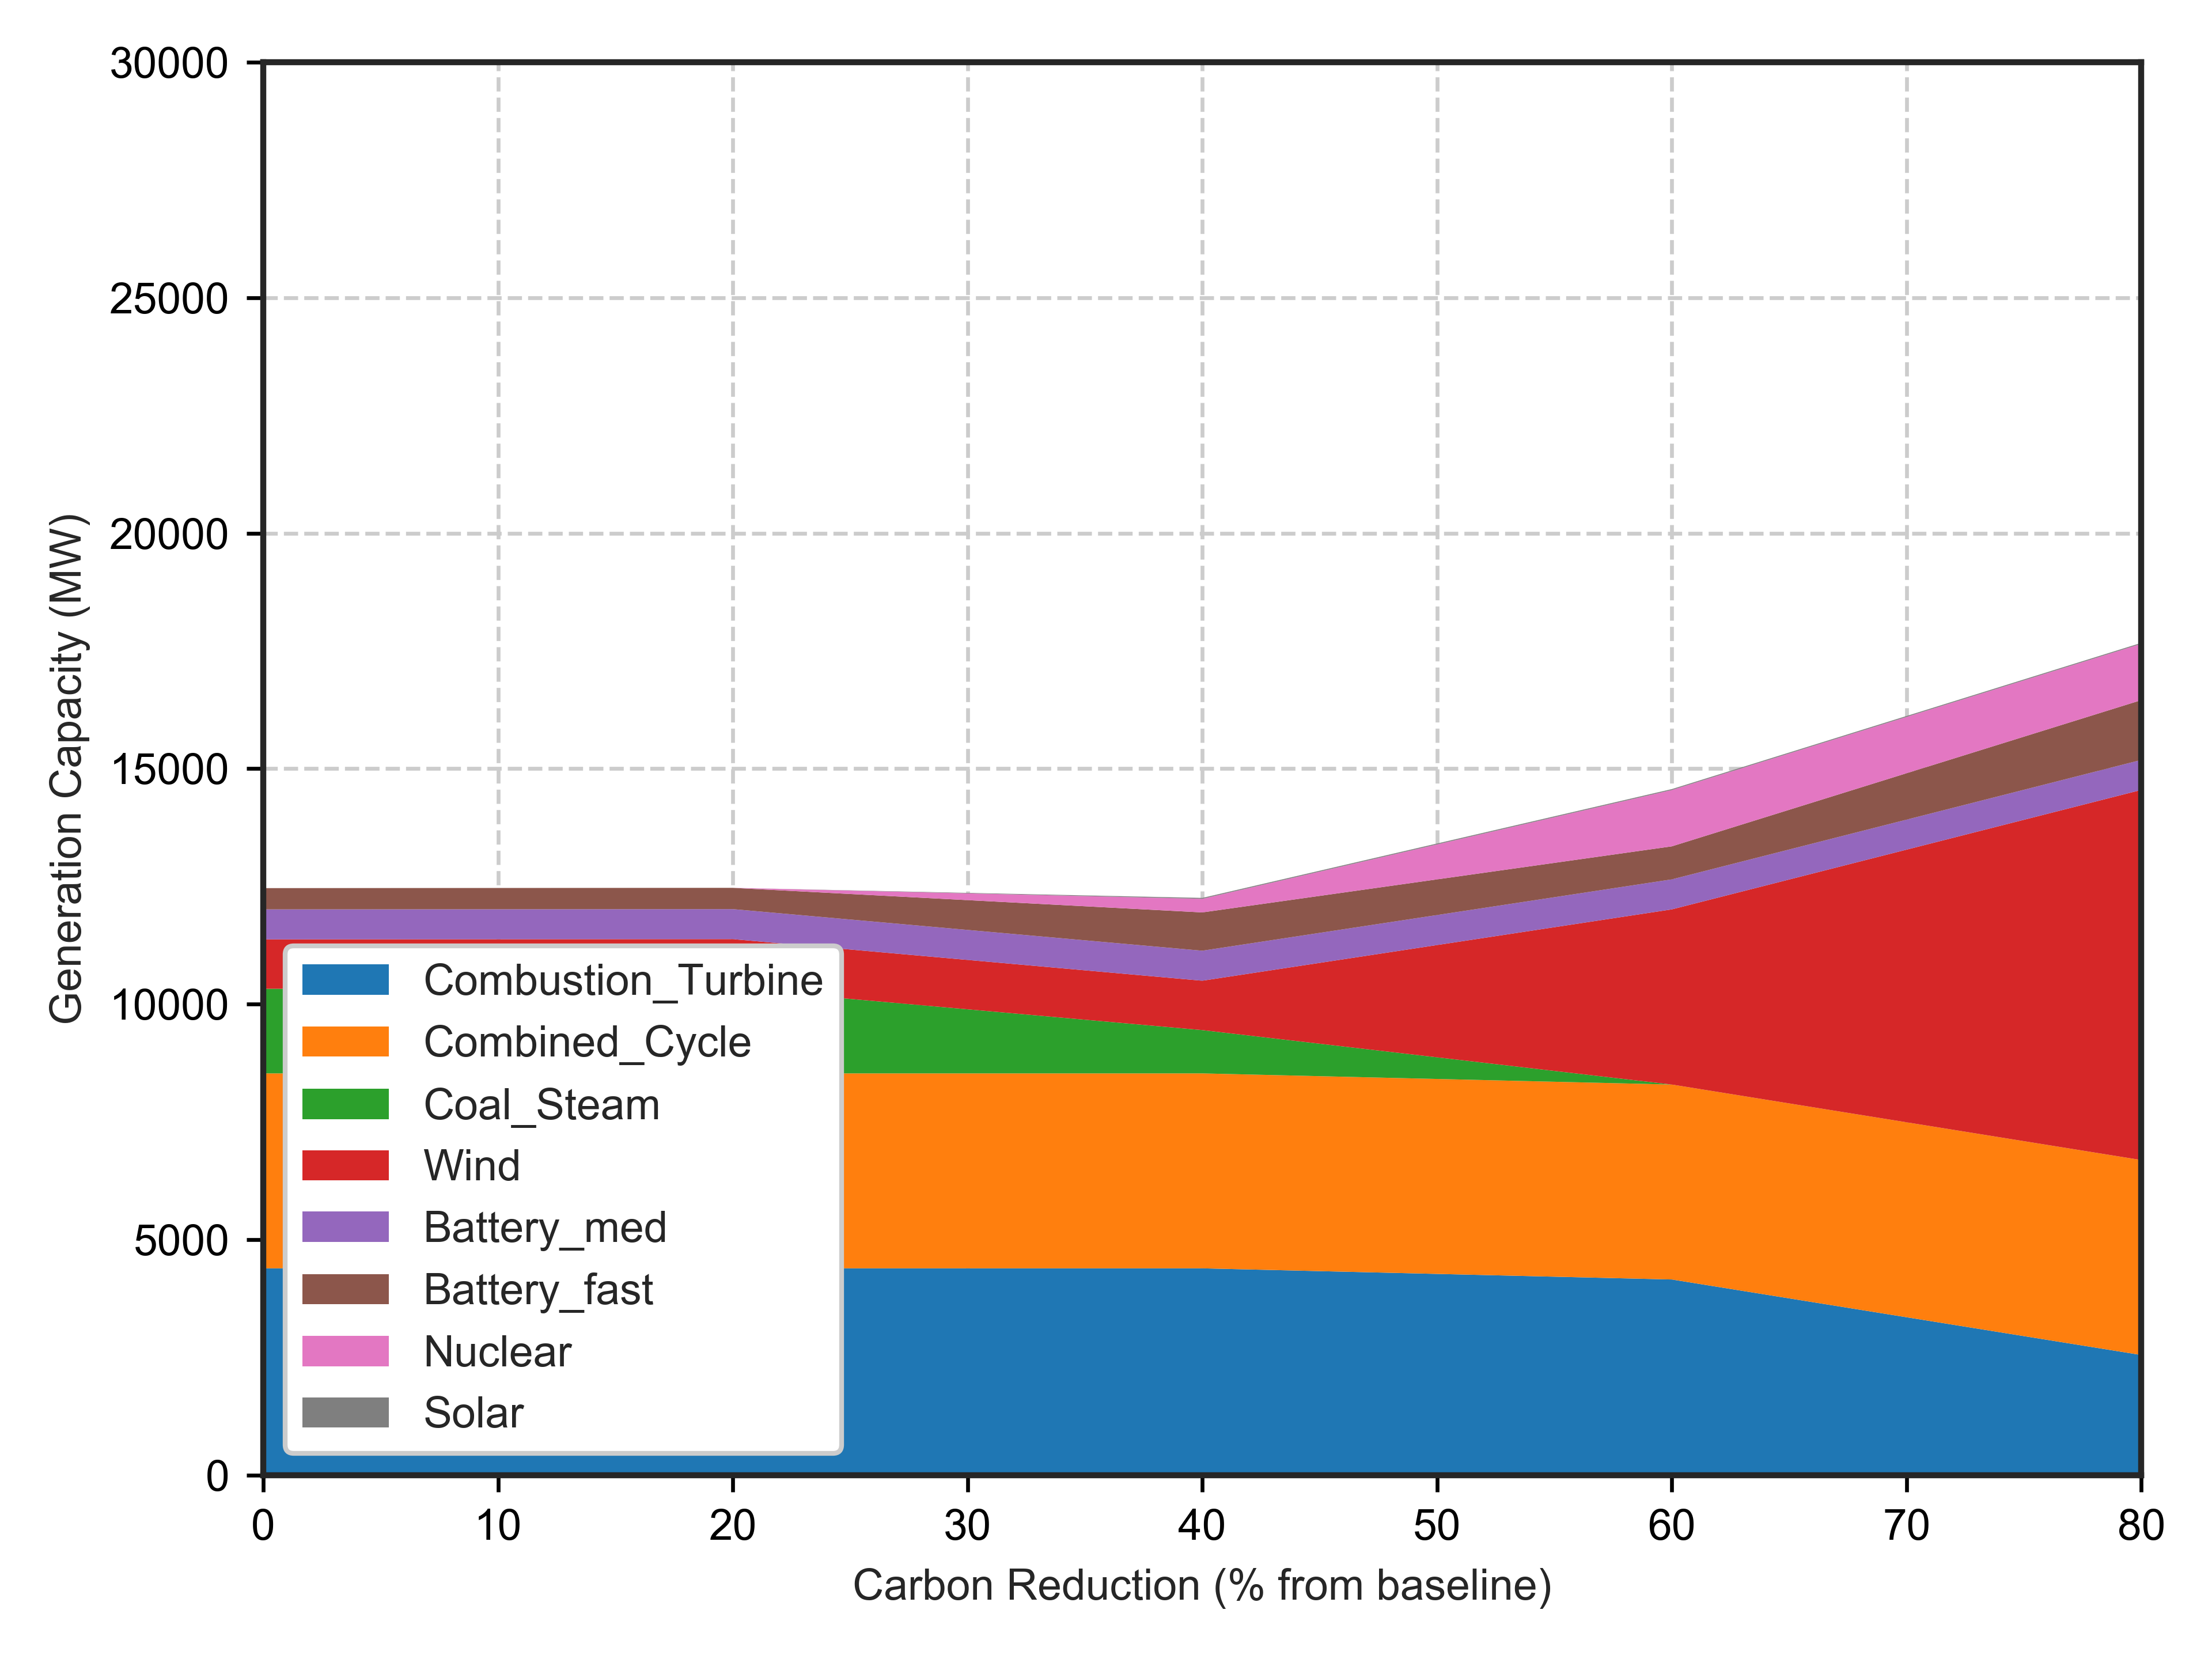
\includegraphics[width=0.32\textwidth]{includes/leakage_shutdowns_agg_capacity_cntlreg.png}
% this is the actual generation for the carbon leak scenario (WI only)
  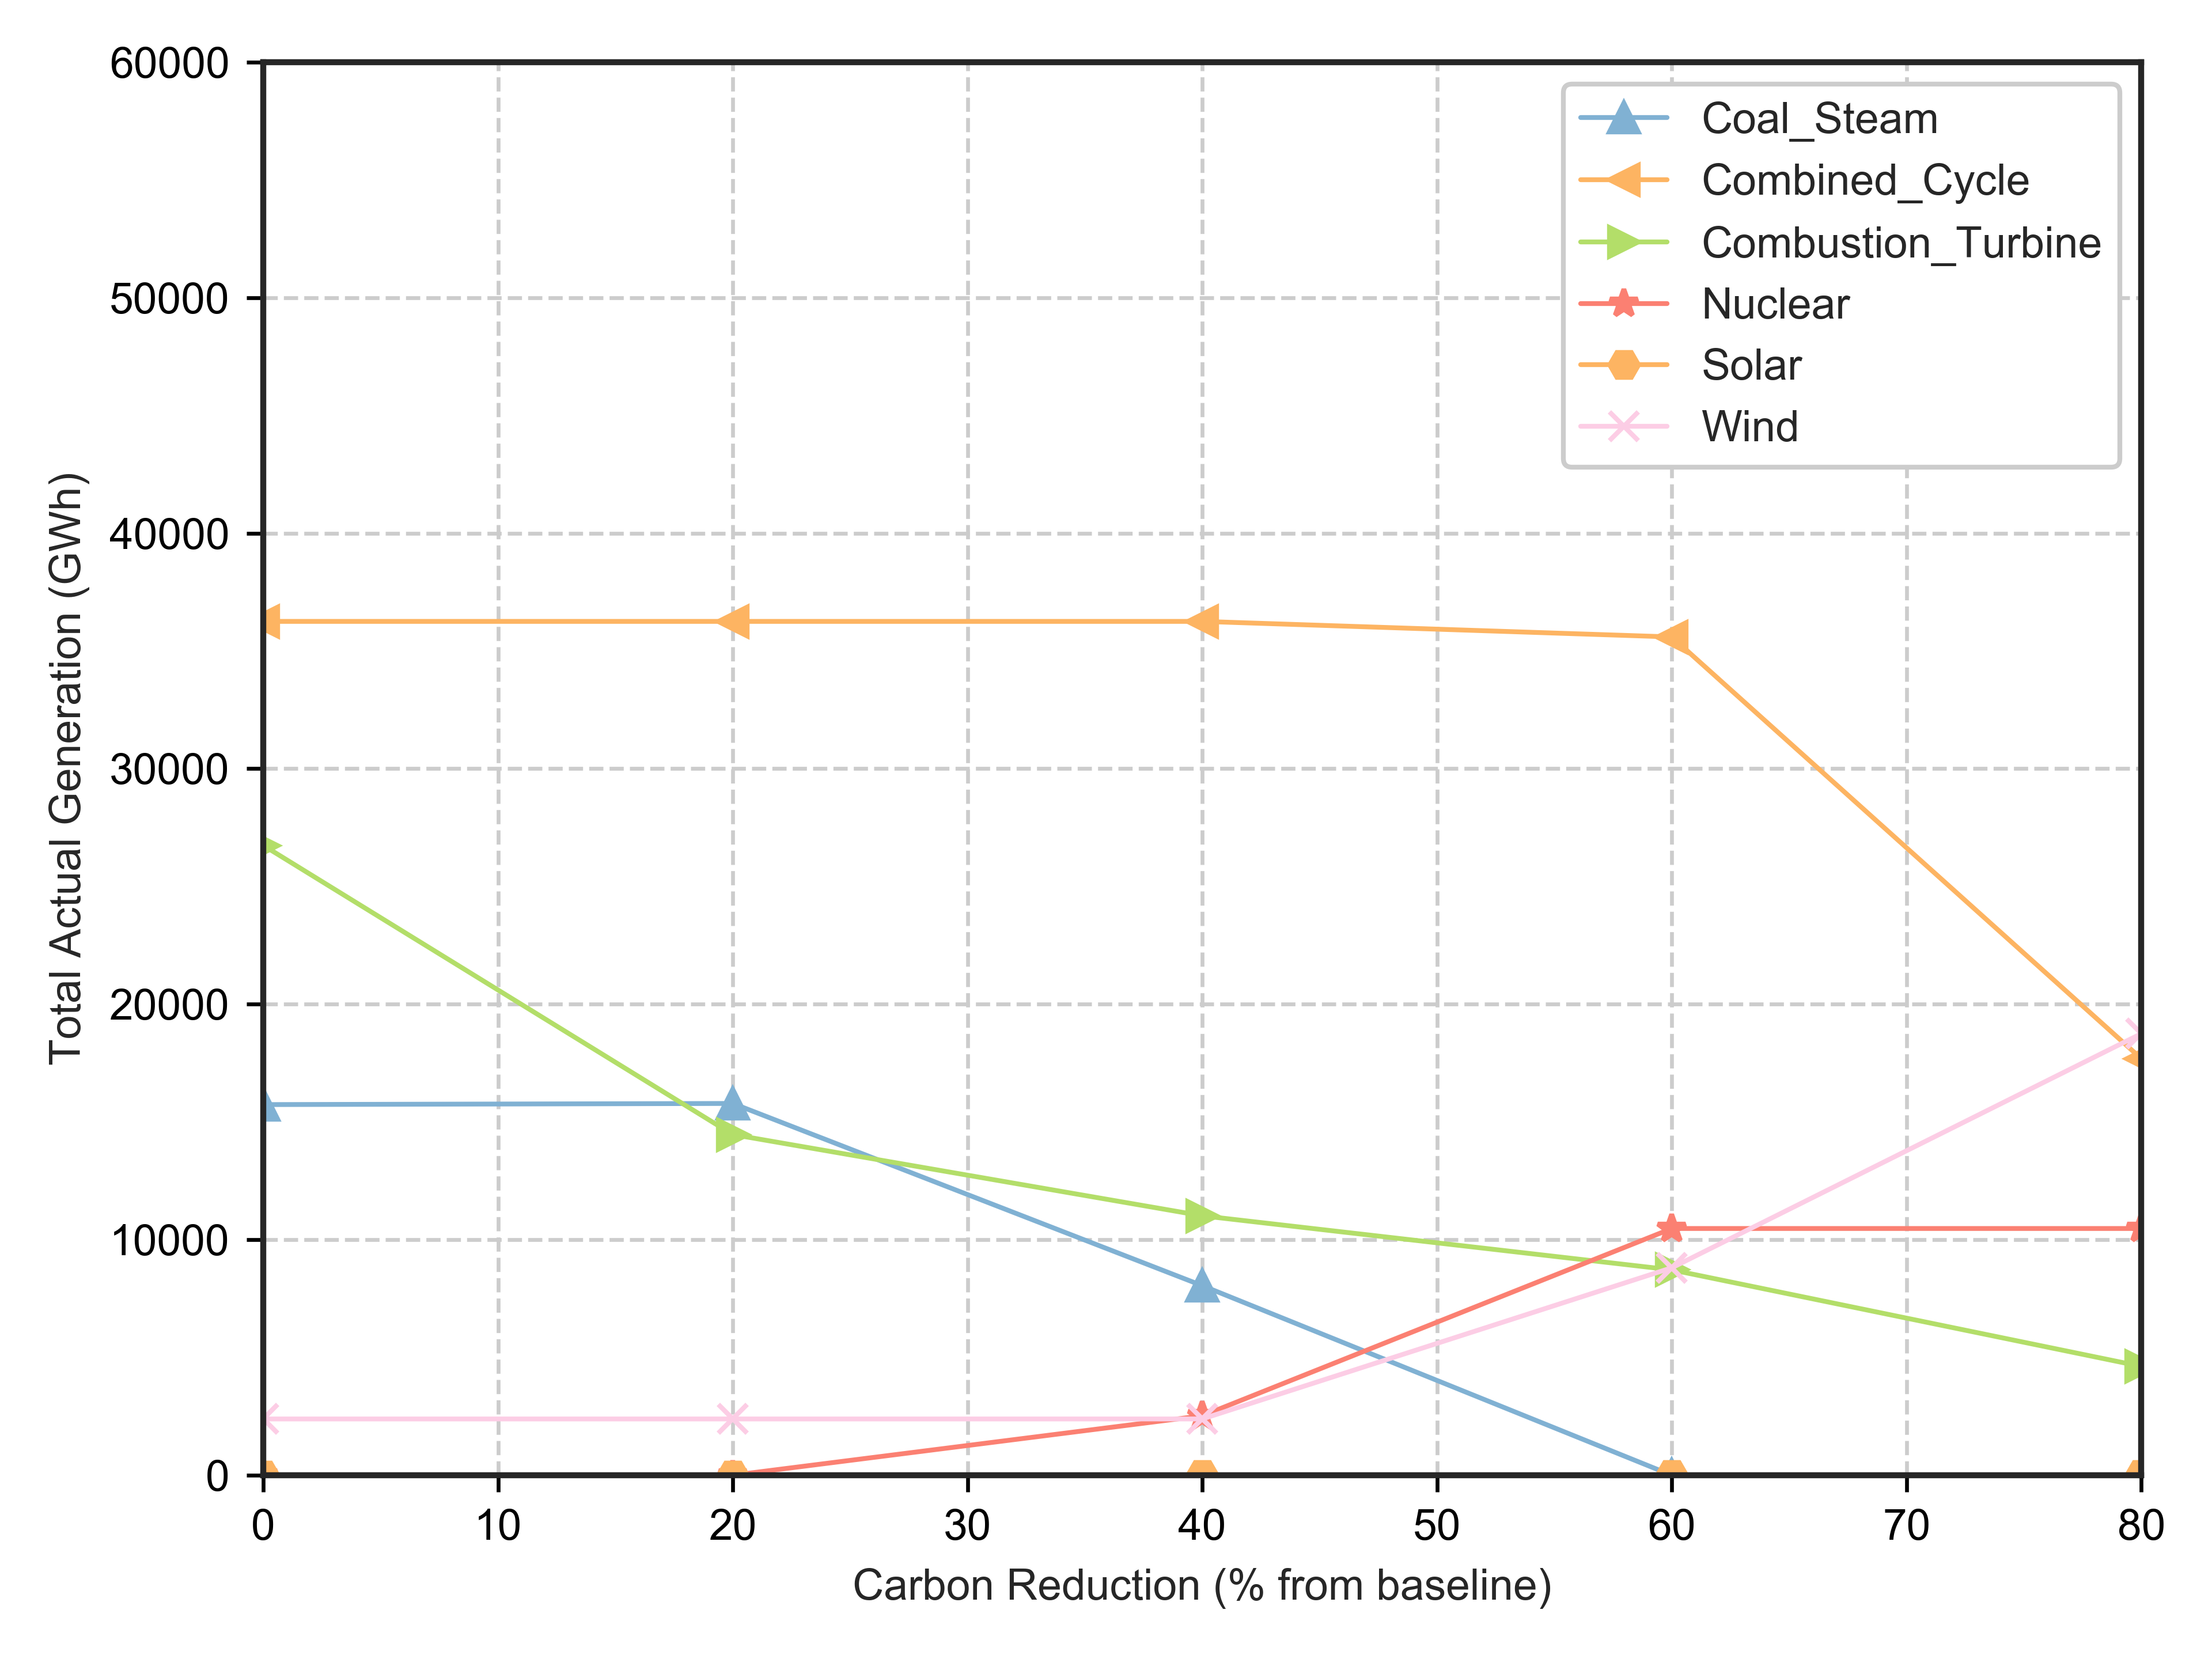
\includegraphics[width=0.32\textwidth]{includes/leakage_shutdowns_agg_generation_cntlreg.png}

  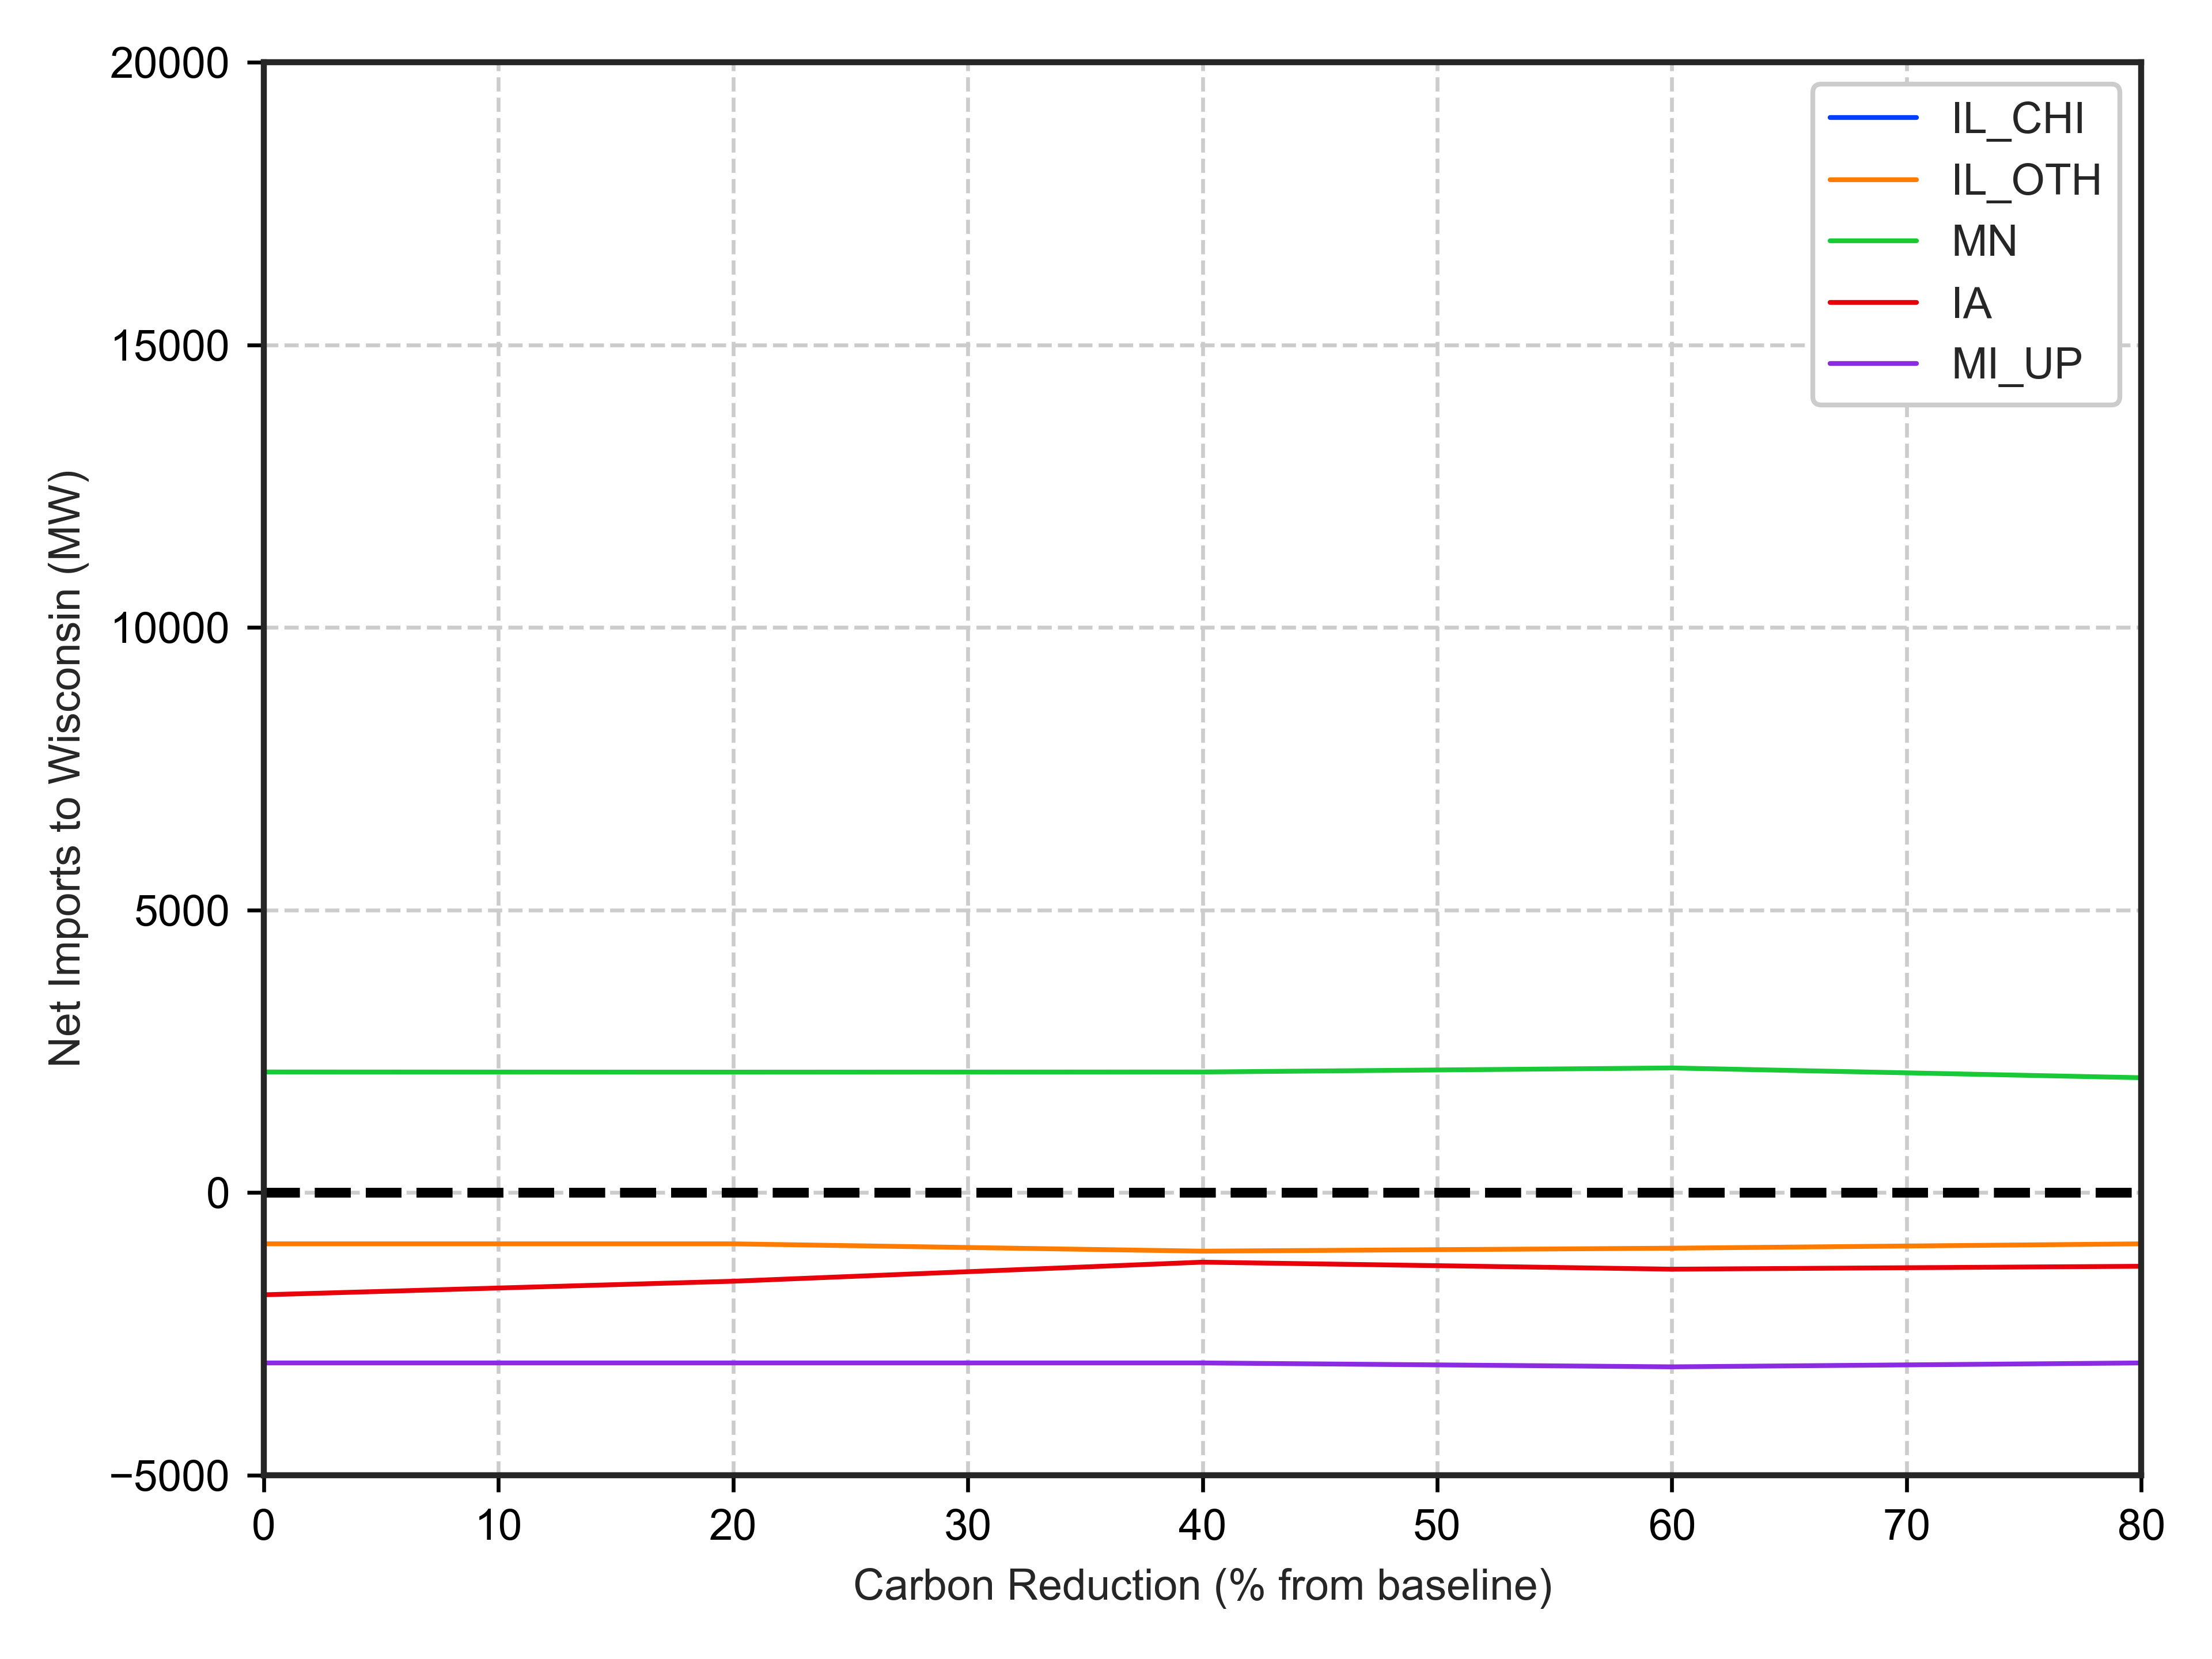
\includegraphics[width=0.32\textwidth]{includes/no_leakage_shutdowns_agg_exim.png}
  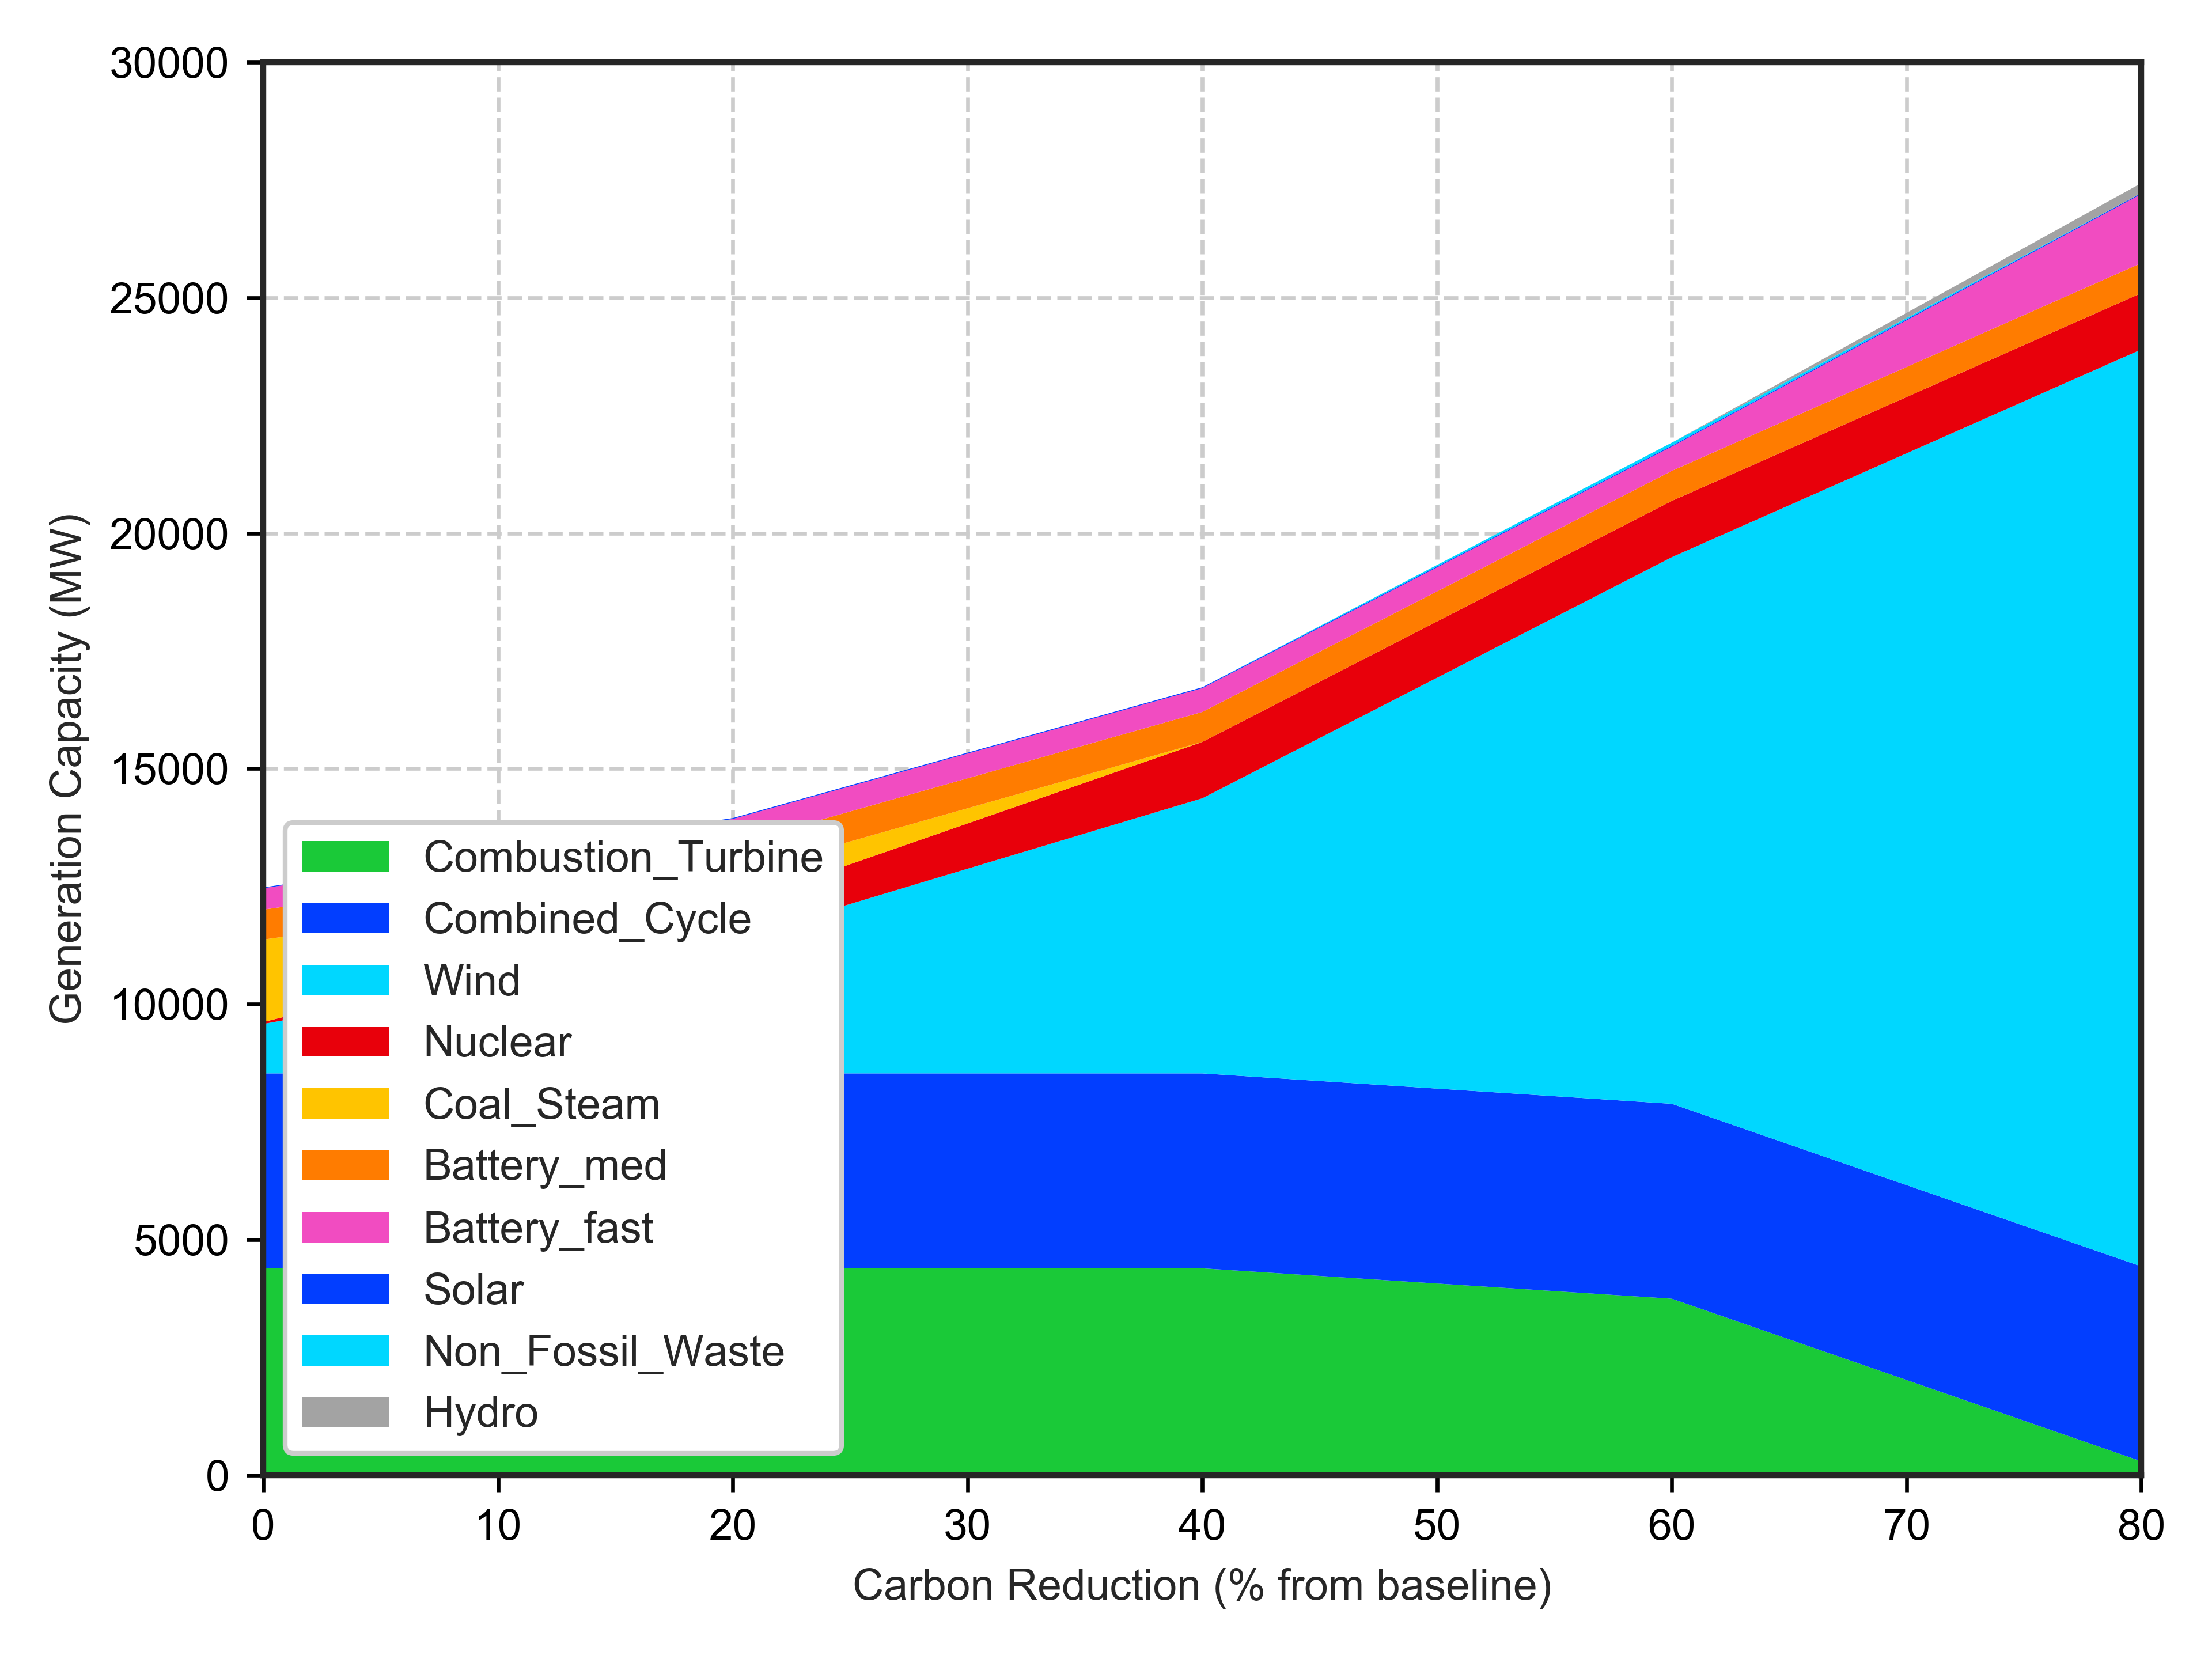
\includegraphics[width=0.32\textwidth]{includes/no_leakage_shutdowns_agg_capacity_cntlreg.png}
% this is the actual generation for the NO carbon leak scenario (WI only)
  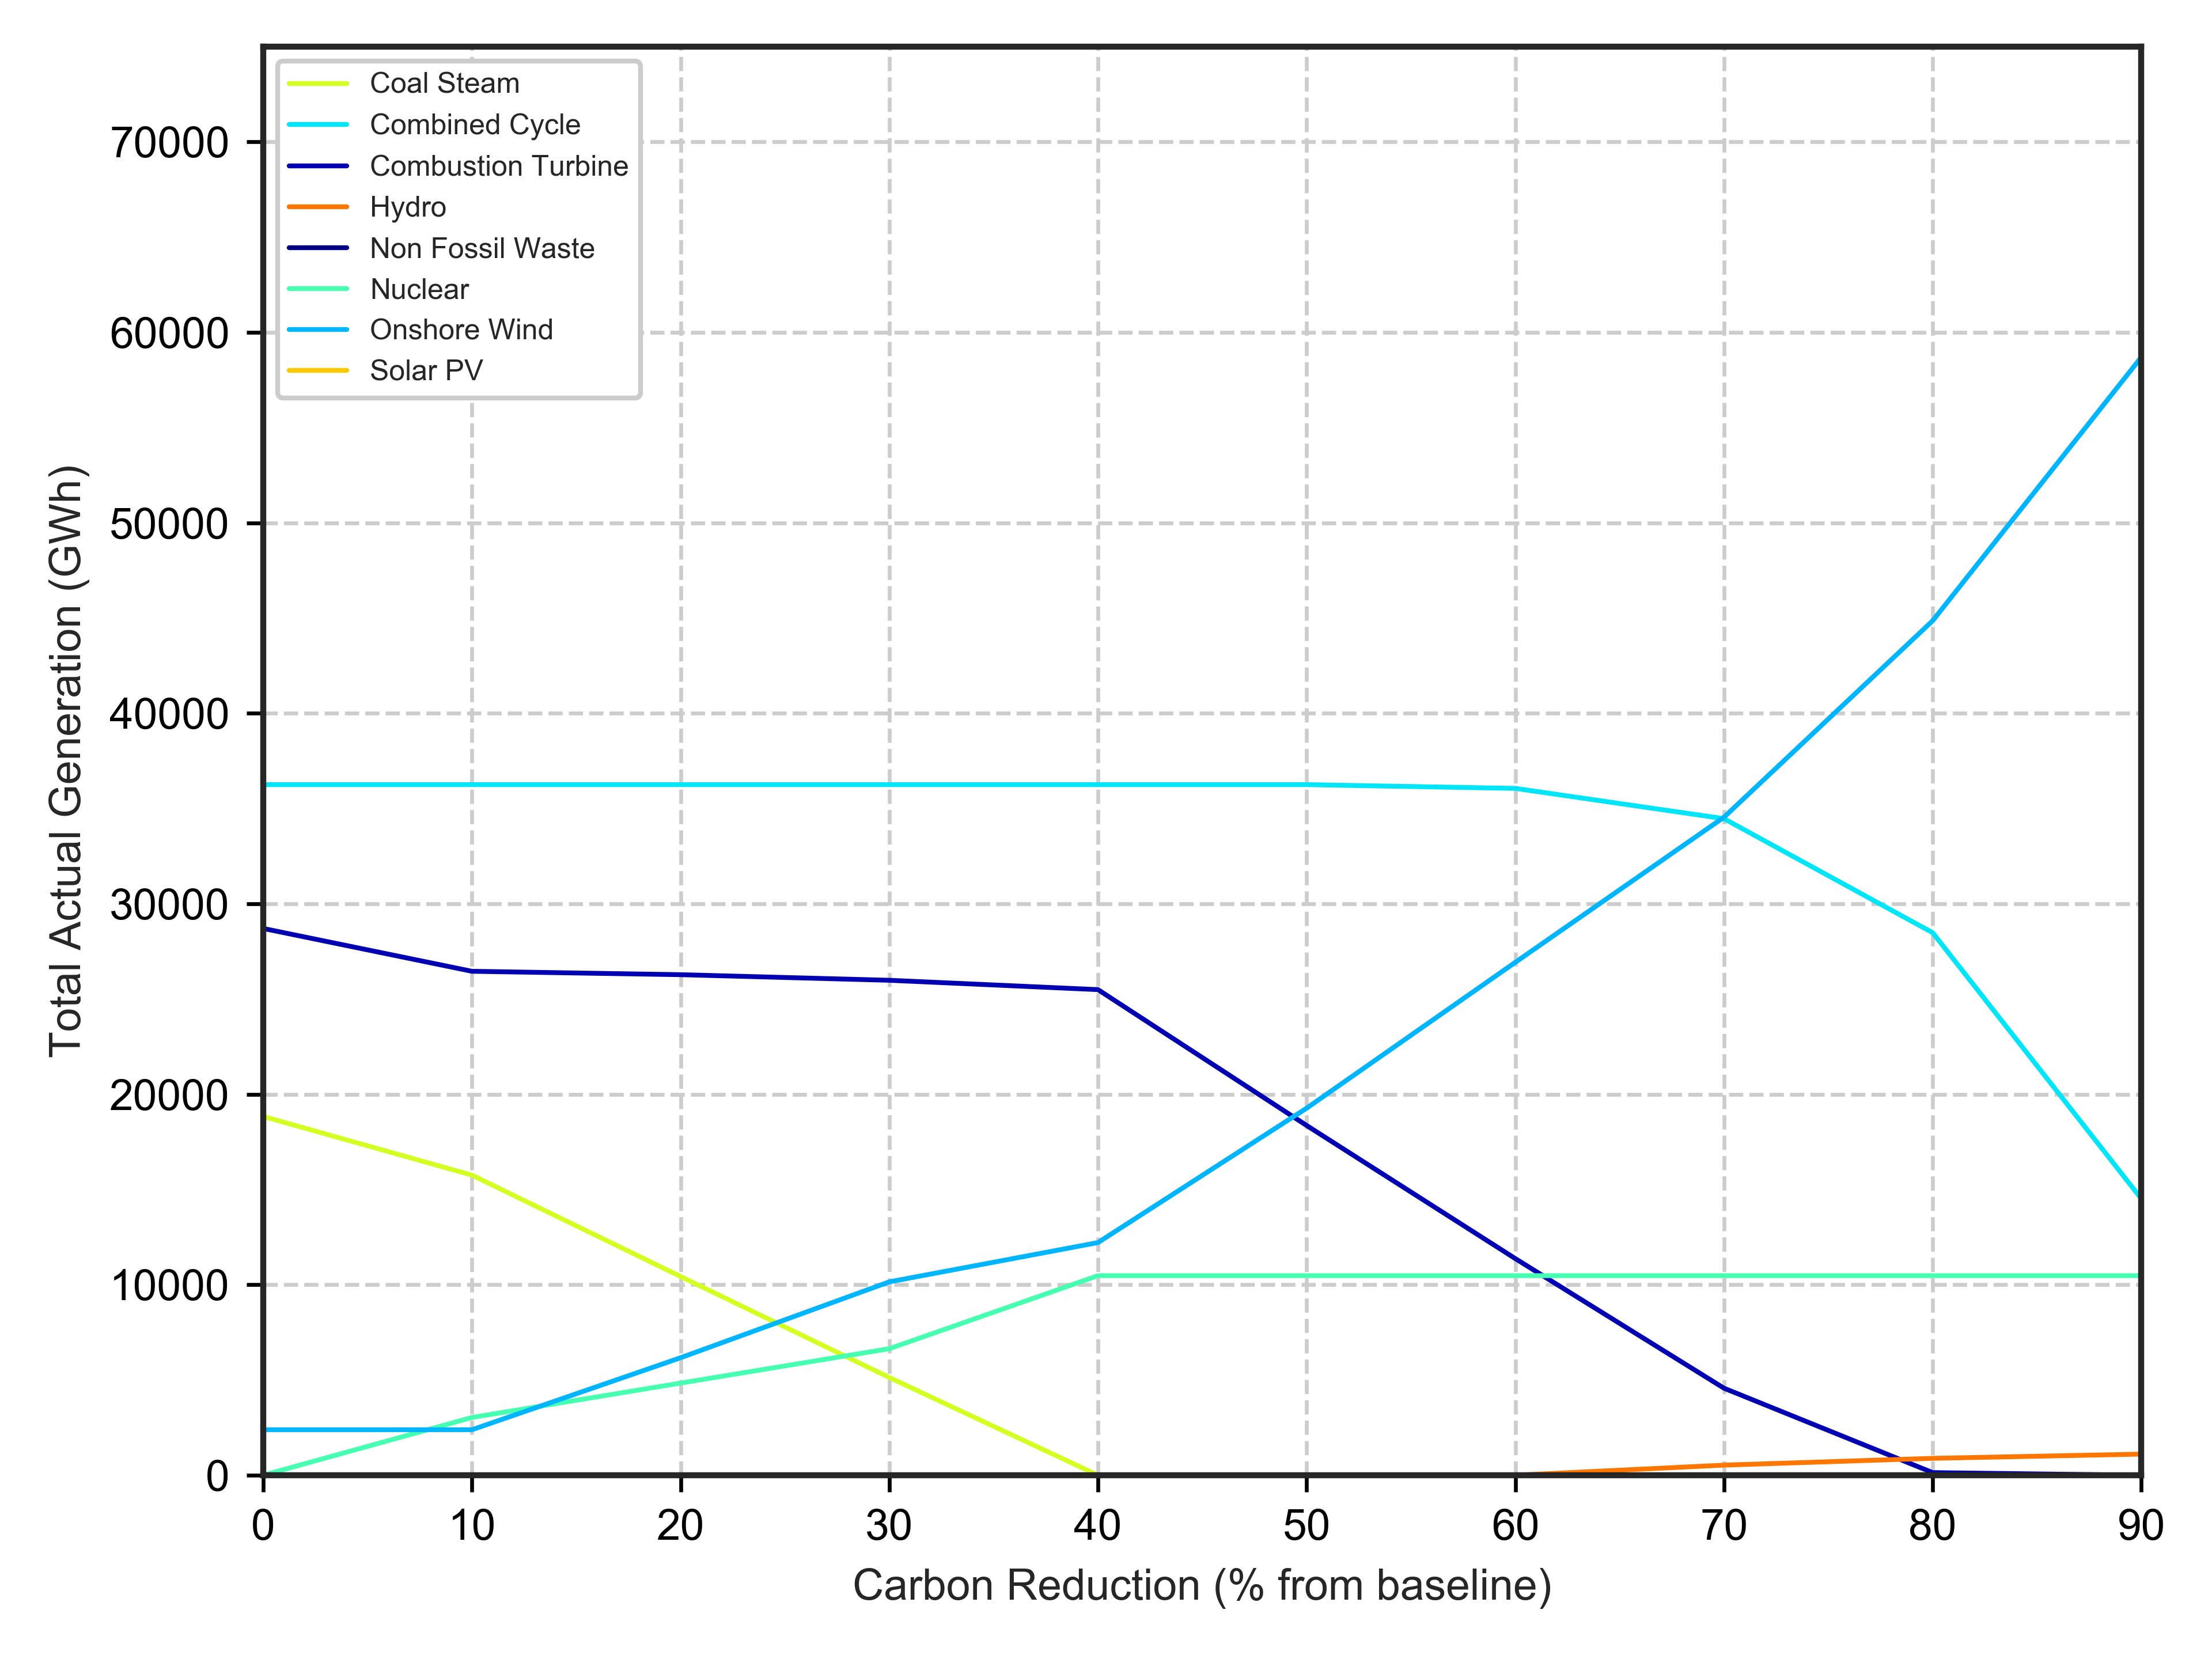
\includegraphics[width=0.32\textwidth]{includes/no_leakage_shutdowns_agg_generation_cntlreg.png}
\end{frame}




% THIS SLIDE SHOWS RESULTS FROM RUNS THAT DID NOT ALLOW SHUTDOWNS
\begin{frame}
%\begin{itemize}
  % this series of maps shows combined cycle generation ramping up and then shutting down.
  % Note that the units here are in % change from baseline for clarity of change

  Combined Cycle (natgas) ramps up and then down while... \\
  % 0% reduction (baseline)
  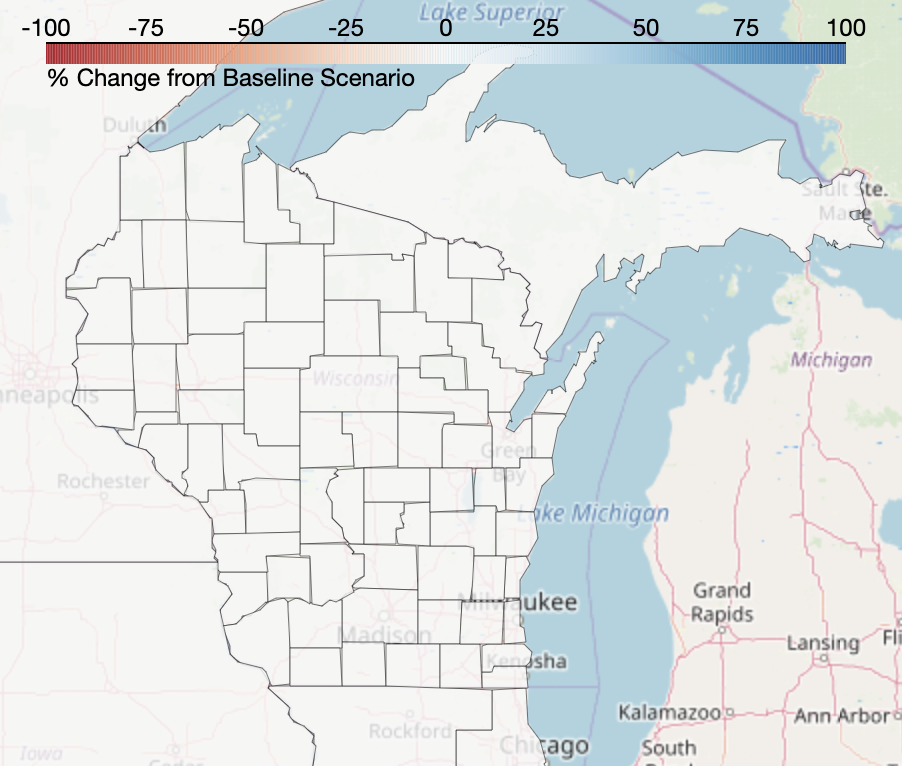
\includegraphics[width=0.25\textwidth]{includes/no_leakage_no_shutdowns_CC_r0.png}
  % 20% reduction
  % 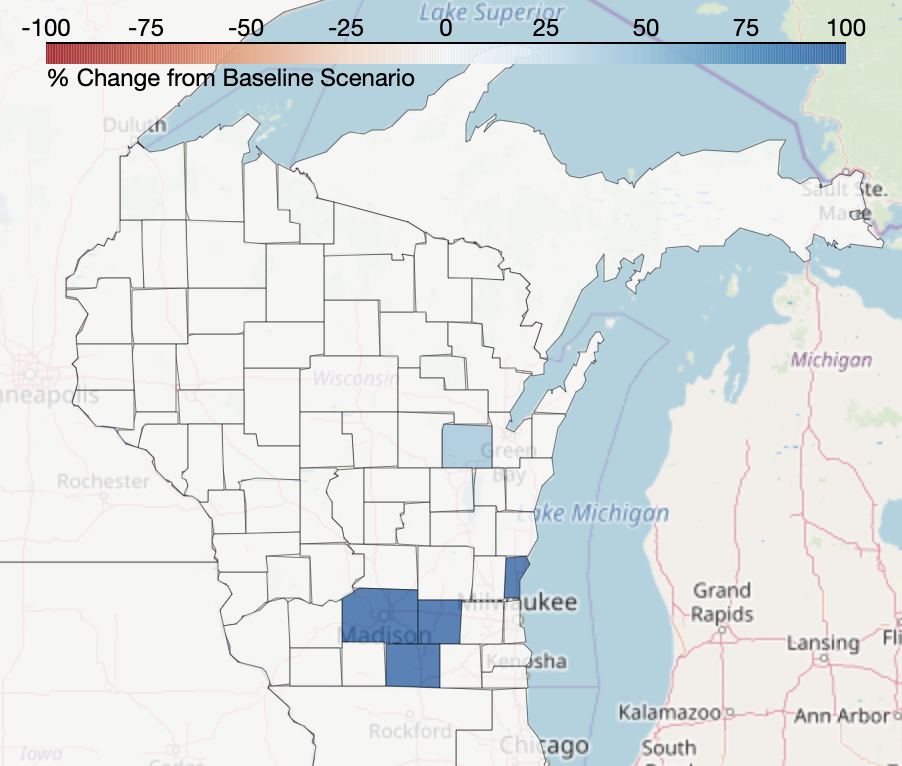
\includegraphics[width=0.25\textwidth]{includes/no_leakage_no_shutdowns_CC_r1.png}
  % 40% reduction
  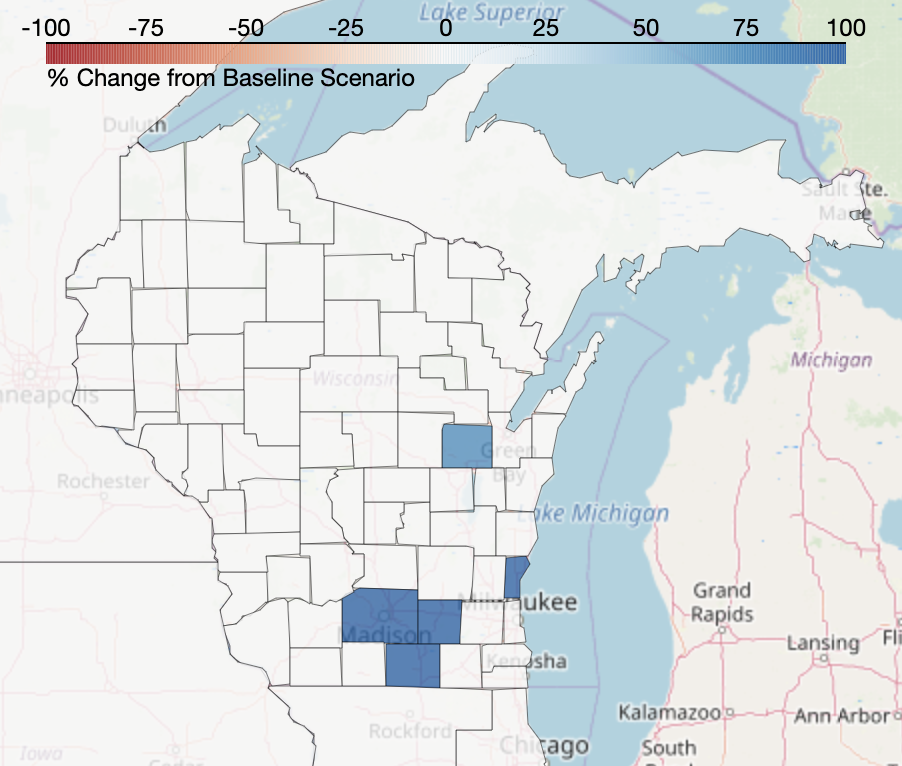
\includegraphics[width=0.25\textwidth]{includes/no_leakage_no_shutdowns_CC_r2.png}
  % 60% reductio
  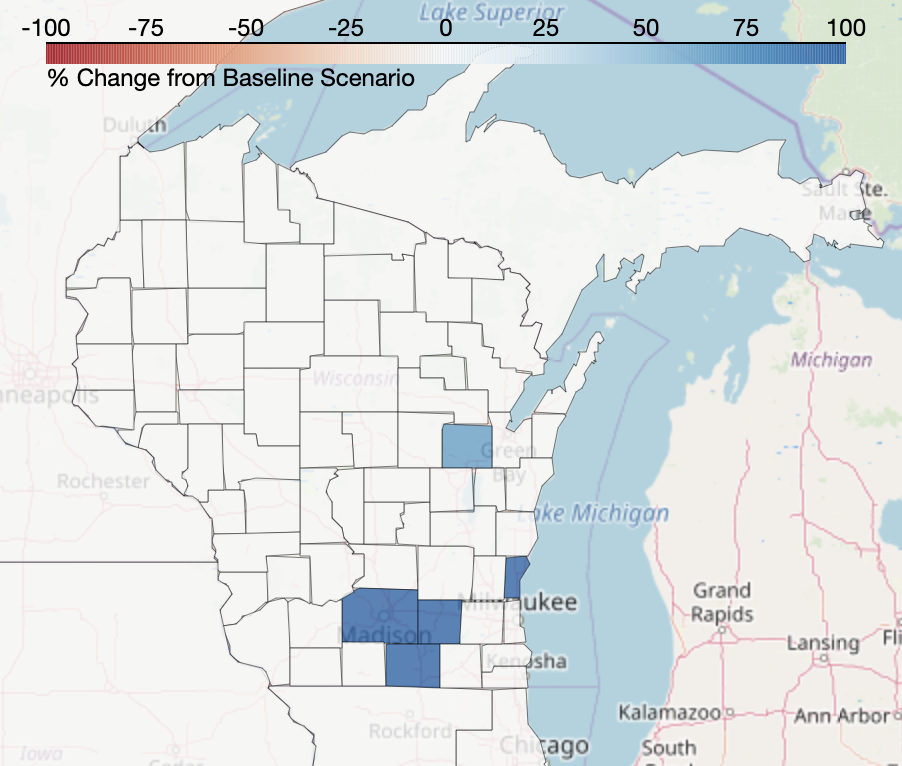
\includegraphics[width=0.25\textwidth]{includes/no_leakage_no_shutdowns_CC_r3.png}
  % 80% reduction
  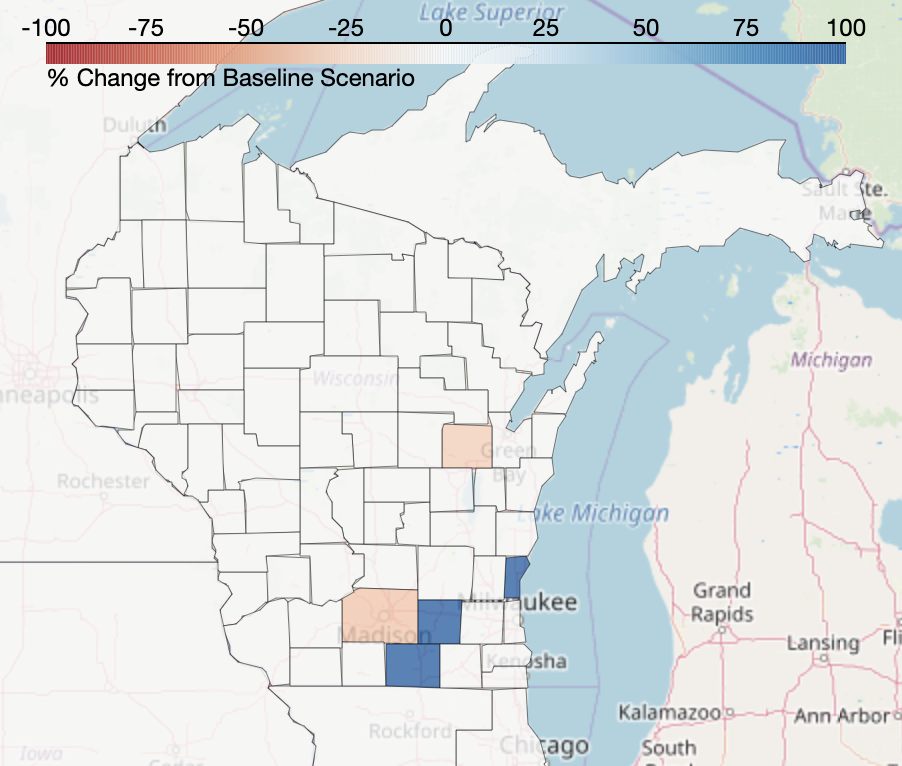
\includegraphics[width=0.25\textwidth]{includes/no_leakage_no_shutdowns_CC_r4.png}

%   % this series of maps shows where wind generation ramps up.
%   % Note that units here are GWh... it shows the change better because most counties in WI do not currently have wind generation which makes calculating the % change from baseline awkward


  Onshore wind ramps up. \\
  % 0% reduction (baseline)
  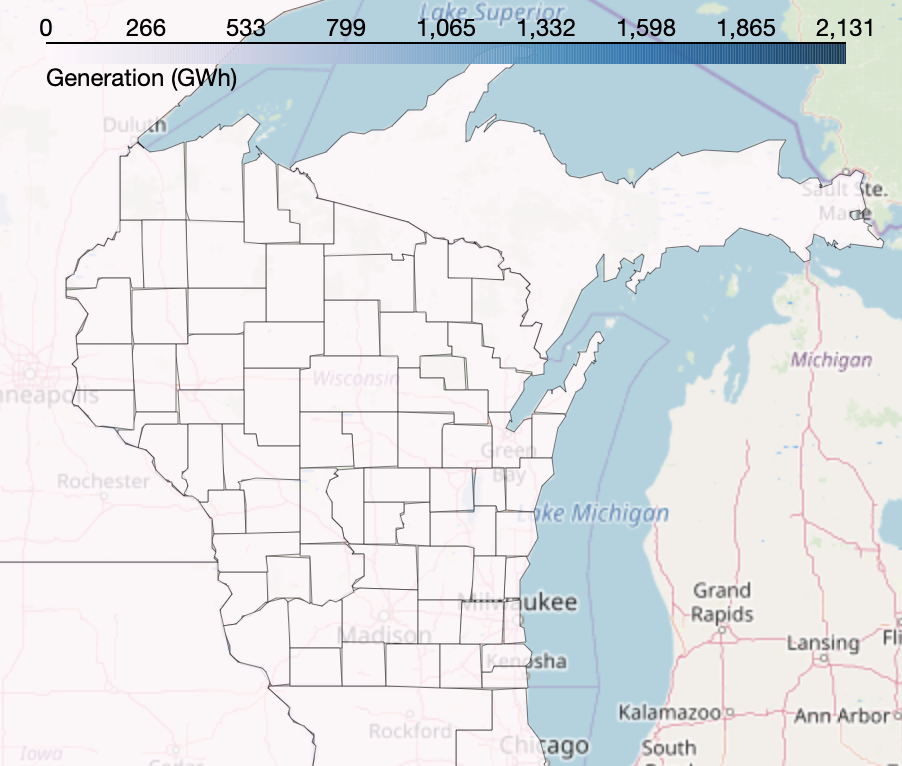
\includegraphics[width=0.25\textwidth]{includes/no_leakage_no_shutdowns_wind_r0.png}
  % 20% reduction
  % 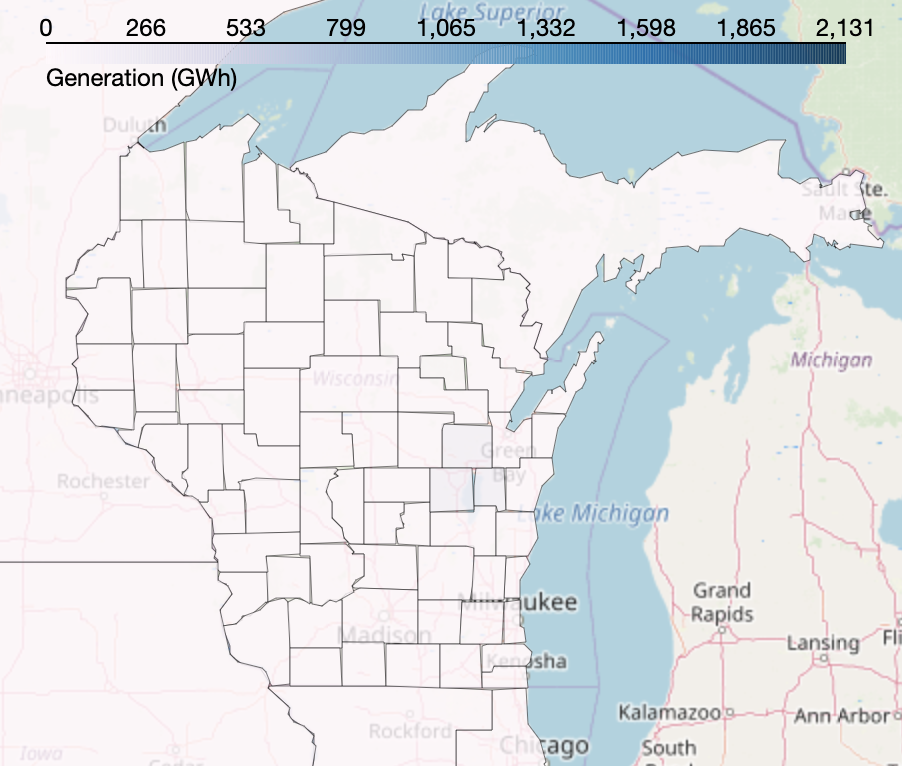
\includegraphics[width=0.25\textwidth]{includes/no_leakage_no_shutdowns_wind_r1.png}
  % 40% reduction
  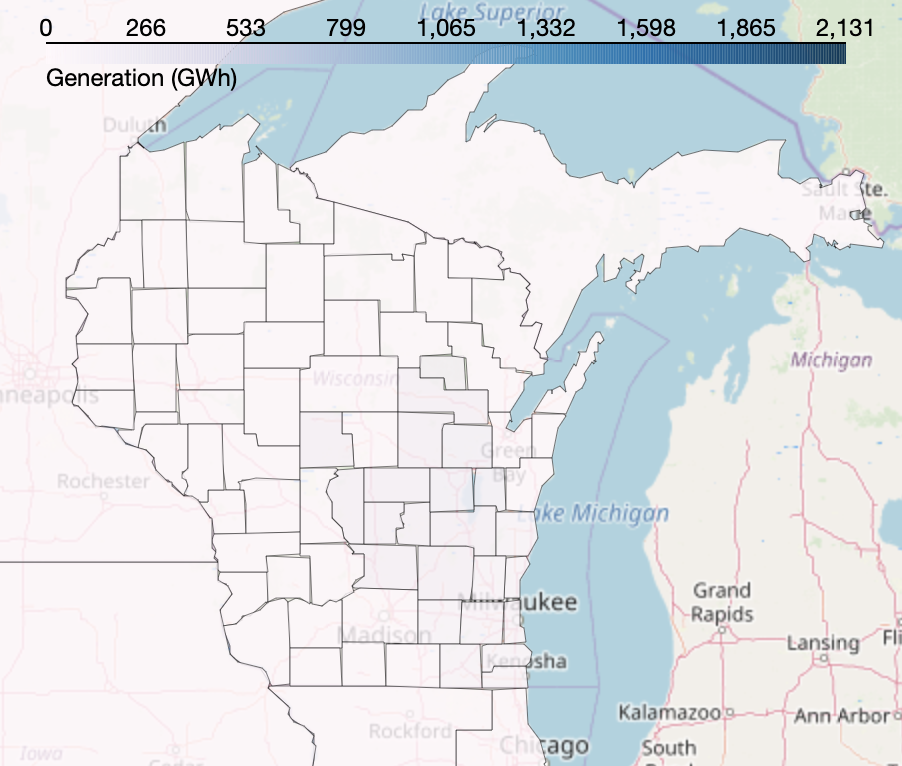
\includegraphics[width=0.25\textwidth]{includes/no_leakage_no_shutdowns_wind_r2.png}
  % 60% reduction
  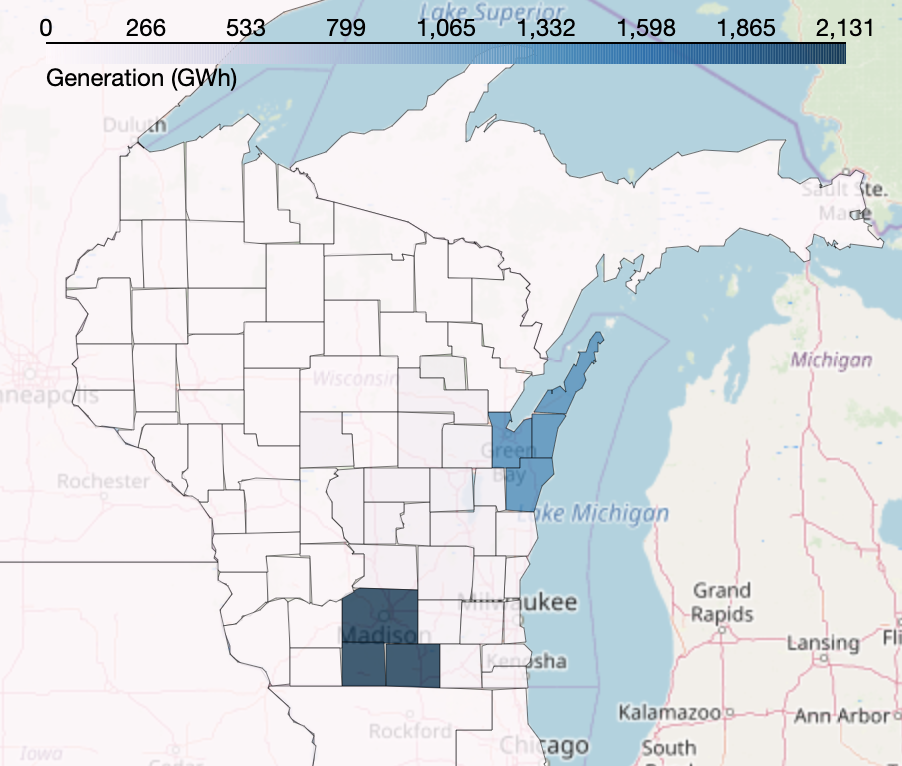
\includegraphics[width=0.25\textwidth]{includes/no_leakage_no_shutdowns_wind_r3.png}
  % 80% reduction
  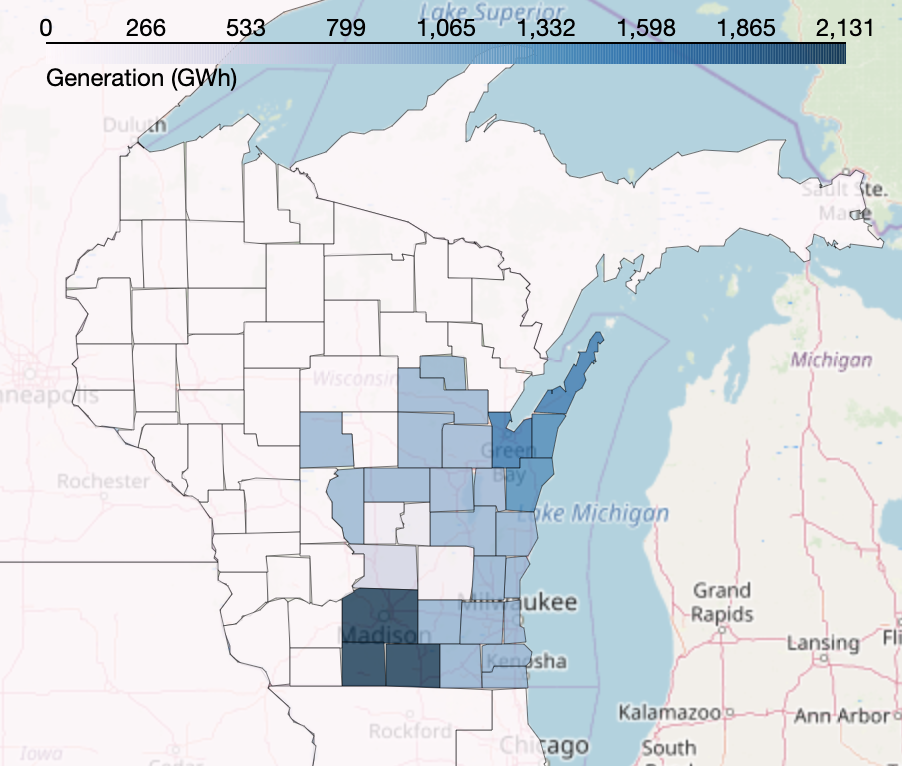
\includegraphics[width=0.25\textwidth]{includes/no_leakage_no_shutdowns_wind_r4.png}
\end{frame}




% THIS SLIDE SHOWS RESULTS FROM RUNS THAT DID ALLOW SHUTDOWNS
\begin{frame}
  \frametitle{Carbon leakage -- Shutdowns Allowed}
  % this series of maps shows combustion turbine generation ramping down.
  Combustion Turbine (natgas) ramps down while... \\
  % 0% reduction (baseline)
  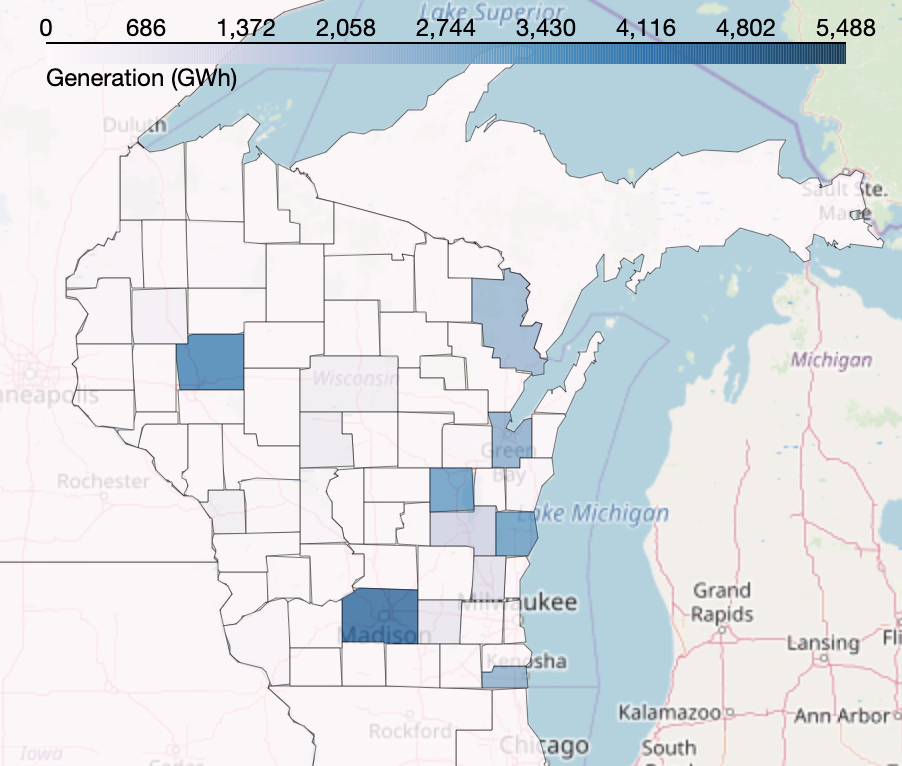
\includegraphics[width=0.25\textwidth]{includes/no_leakage_shutdowns_CT_r0.png}
  % 20% reduction
  % 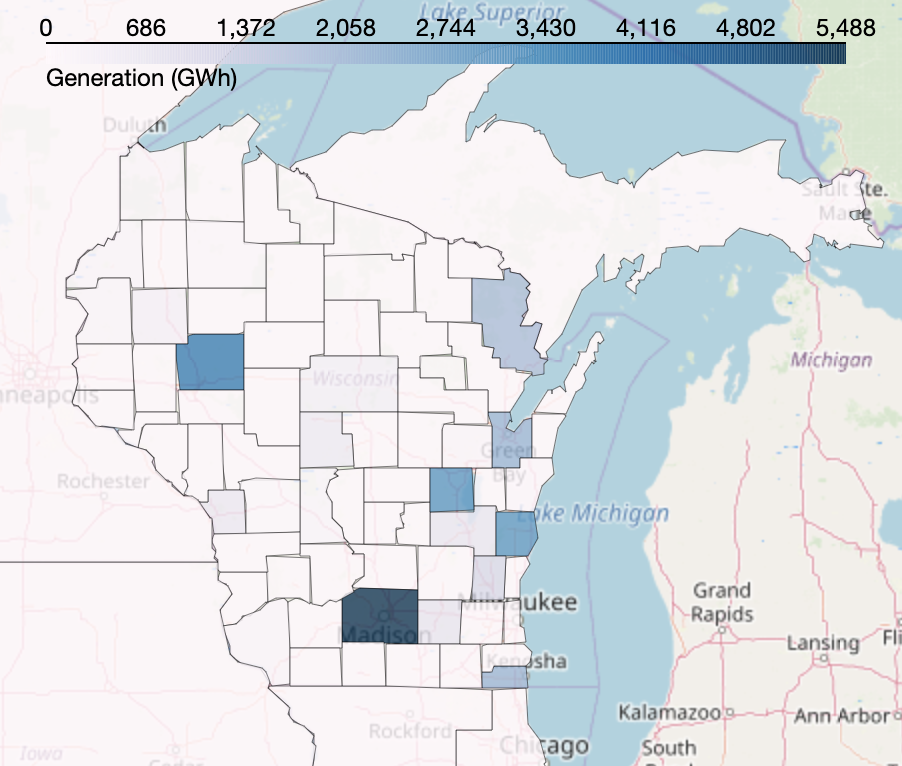
\includegraphics[width=0.25\textwidth]{includes/no_leakage_shutdowns_CT_r1.png}
  % 40% reduction
  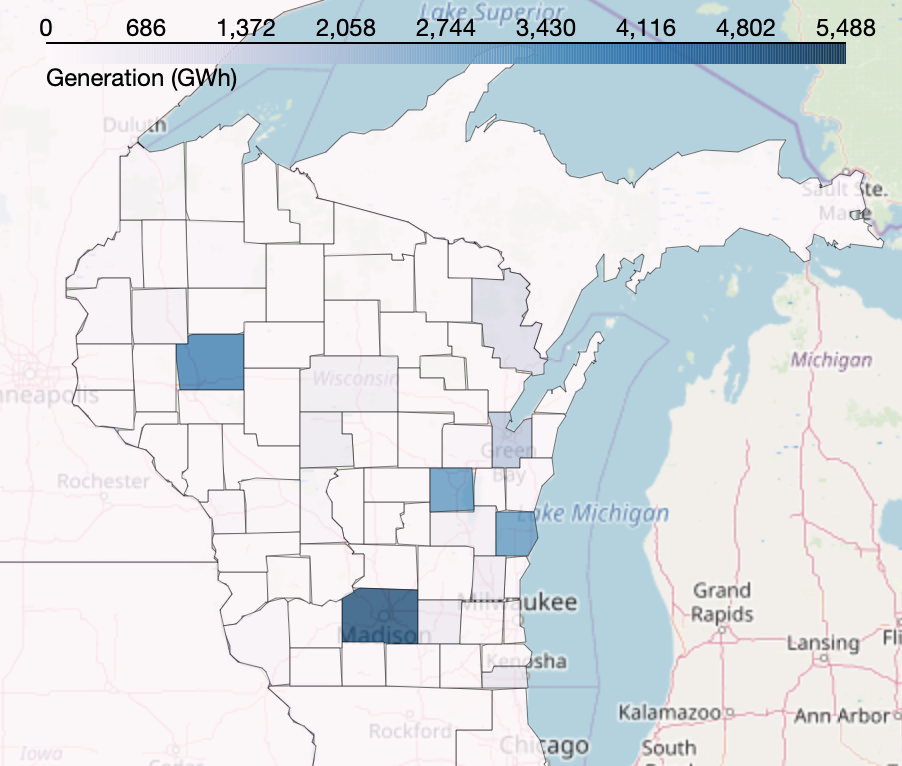
\includegraphics[width=0.25\textwidth]{includes/no_leakage_shutdowns_CT_r2.png}
  % 60% reduction
  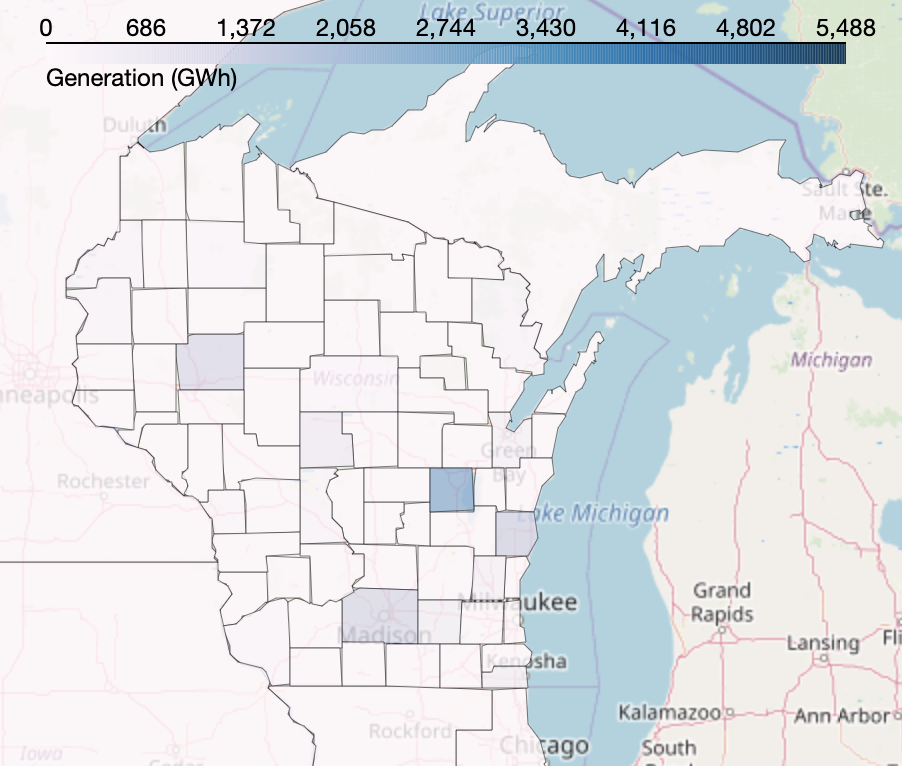
\includegraphics[width=0.25\textwidth]{includes/no_leakage_shutdowns_CT_r3.png}
  % 80% reduction
  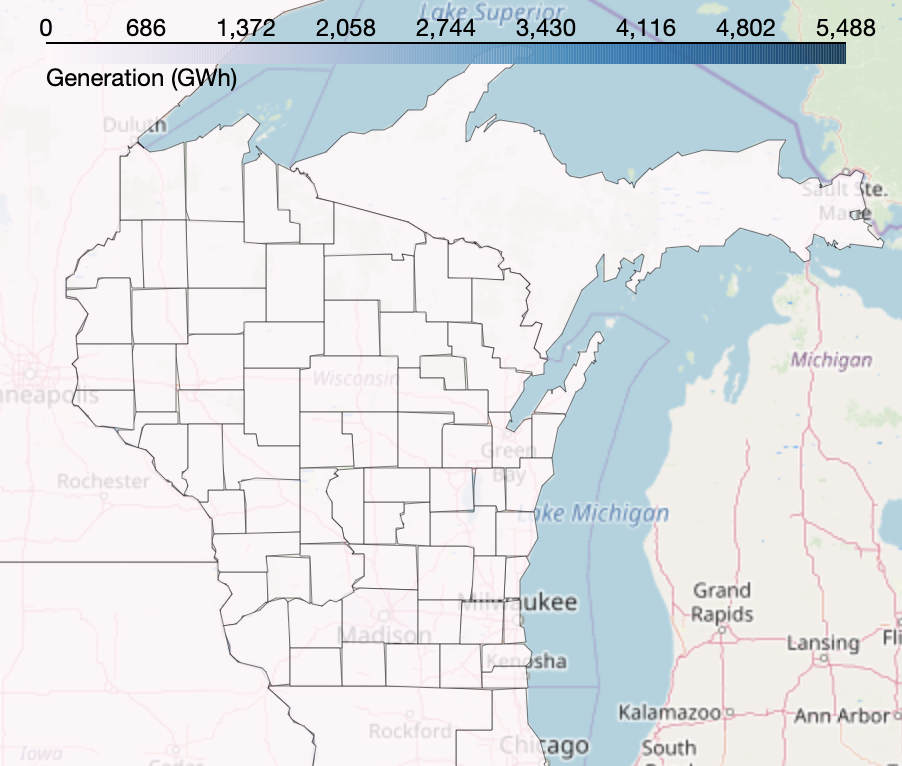
\includegraphics[width=0.25\textwidth]{includes/no_leakage_shutdowns_CT_r4.png}

  % Note that units here are GWh... it shows the change better because most counties in WI do not currently have wind generation which makes calculating the % change from baseline awkward
  Onshore wind ramps up.\\
  % 0% reduction (baseline)
  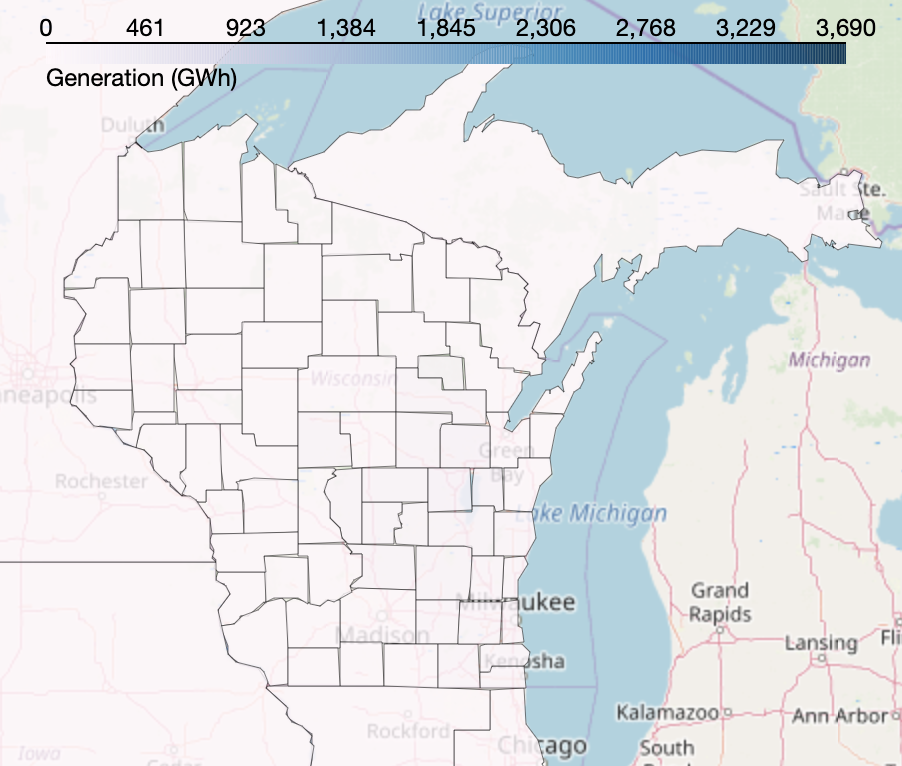
\includegraphics[width=0.25\textwidth]{includes/no_leakage_shutdowns_wind_r0.png}
  % 20% reduction
  % 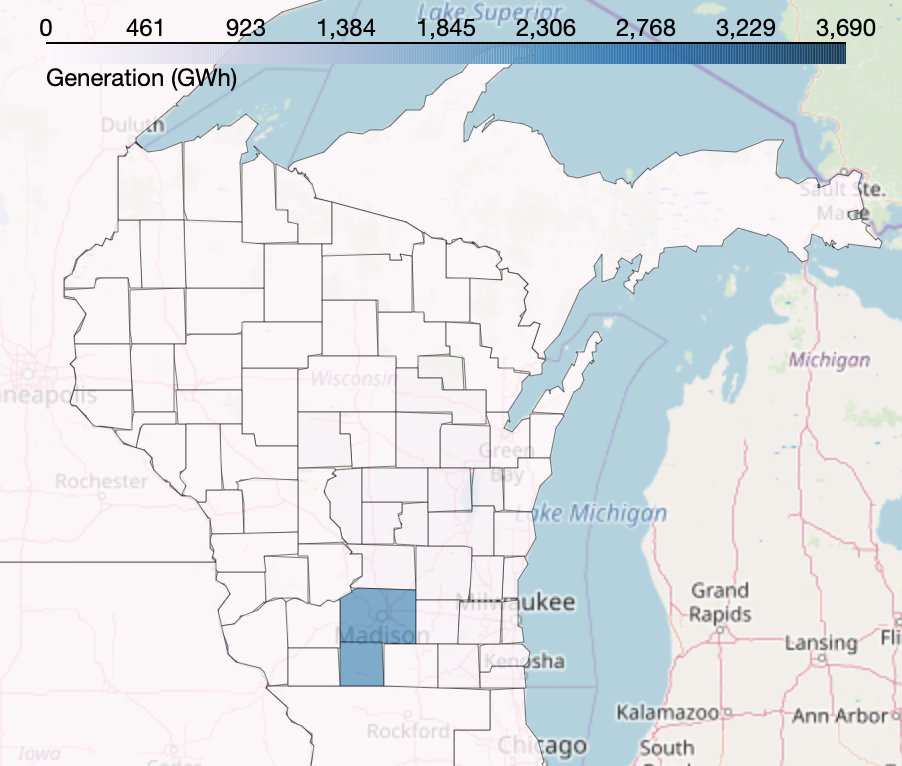
\includegraphics[width=0.25\textwidth]{includes/no_leakage_shutdowns_wind_r1.png}
  % 40% reduction
  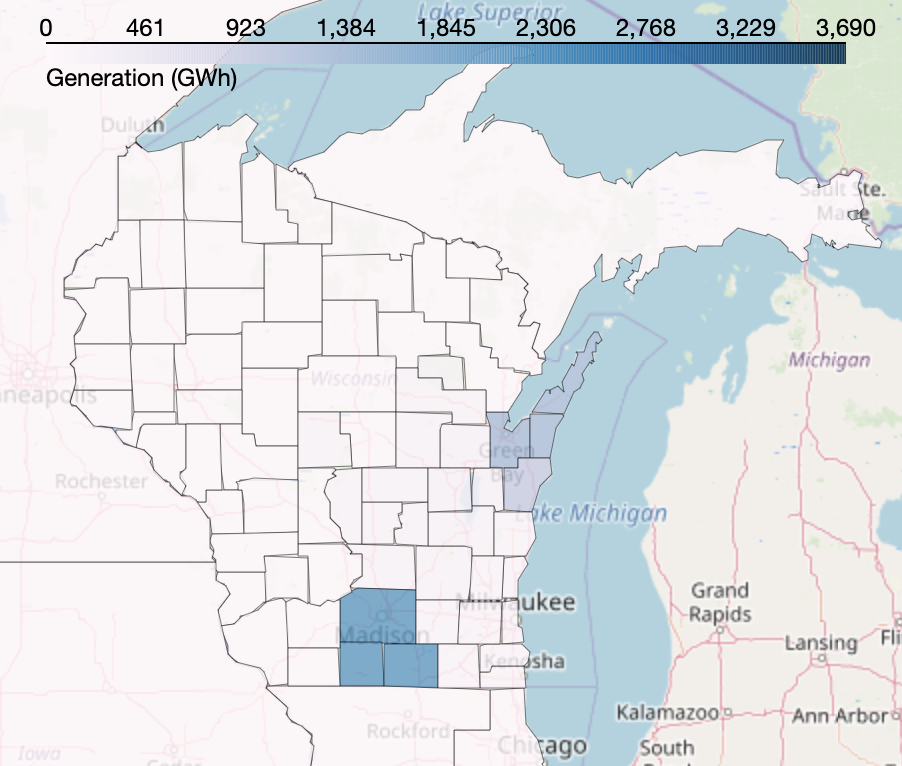
\includegraphics[width=0.25\textwidth]{includes/no_leakage_shutdowns_wind_r2.png}
  % 60% reduction
  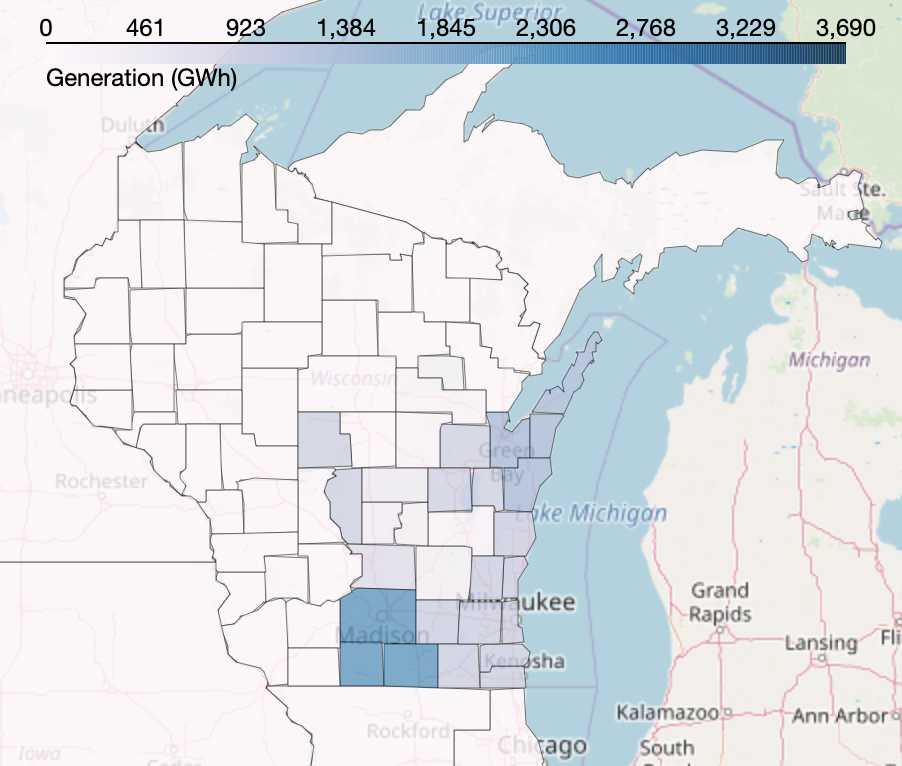
\includegraphics[width=0.25\textwidth]{includes/no_leakage_shutdowns_wind_r3.png}
  % 80% reduction
  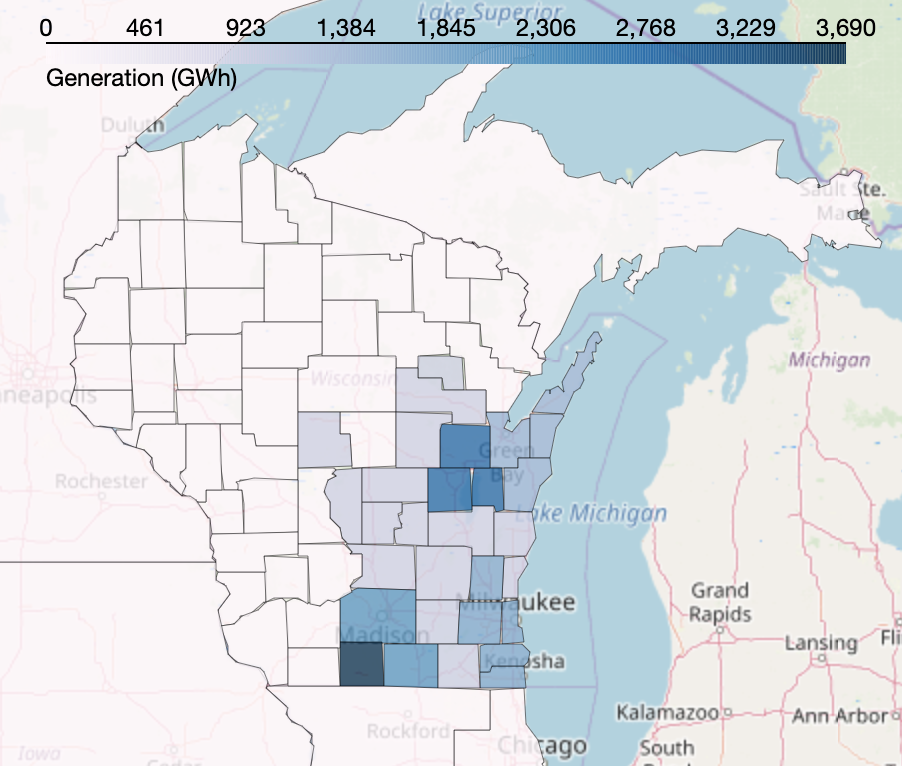
\includegraphics[width=0.25\textwidth]{includes/no_leakage_shutdowns_wind_r4.png}
\end{frame}


\begin{frame}
  \frametitle{Increased demand -- Shutdowns Allowed}

\begin{itemize}
  \item Cost effects (and possible changes in portfolio of generation) when
have increased demand.  Flat imports. Shutdowns allowed
  \item 5\% increase in demand for WI only (beyond the growth factor for 2030)
  \item Wind still dominates the low carbon fuel, but the demand shock incentivizes nuclear to come in back in earlier ($>20$\%)
  \item Carbon emissions policy baseline is set in 2020 -- more demand but same emissions cap necessitates lots of clean electricity

  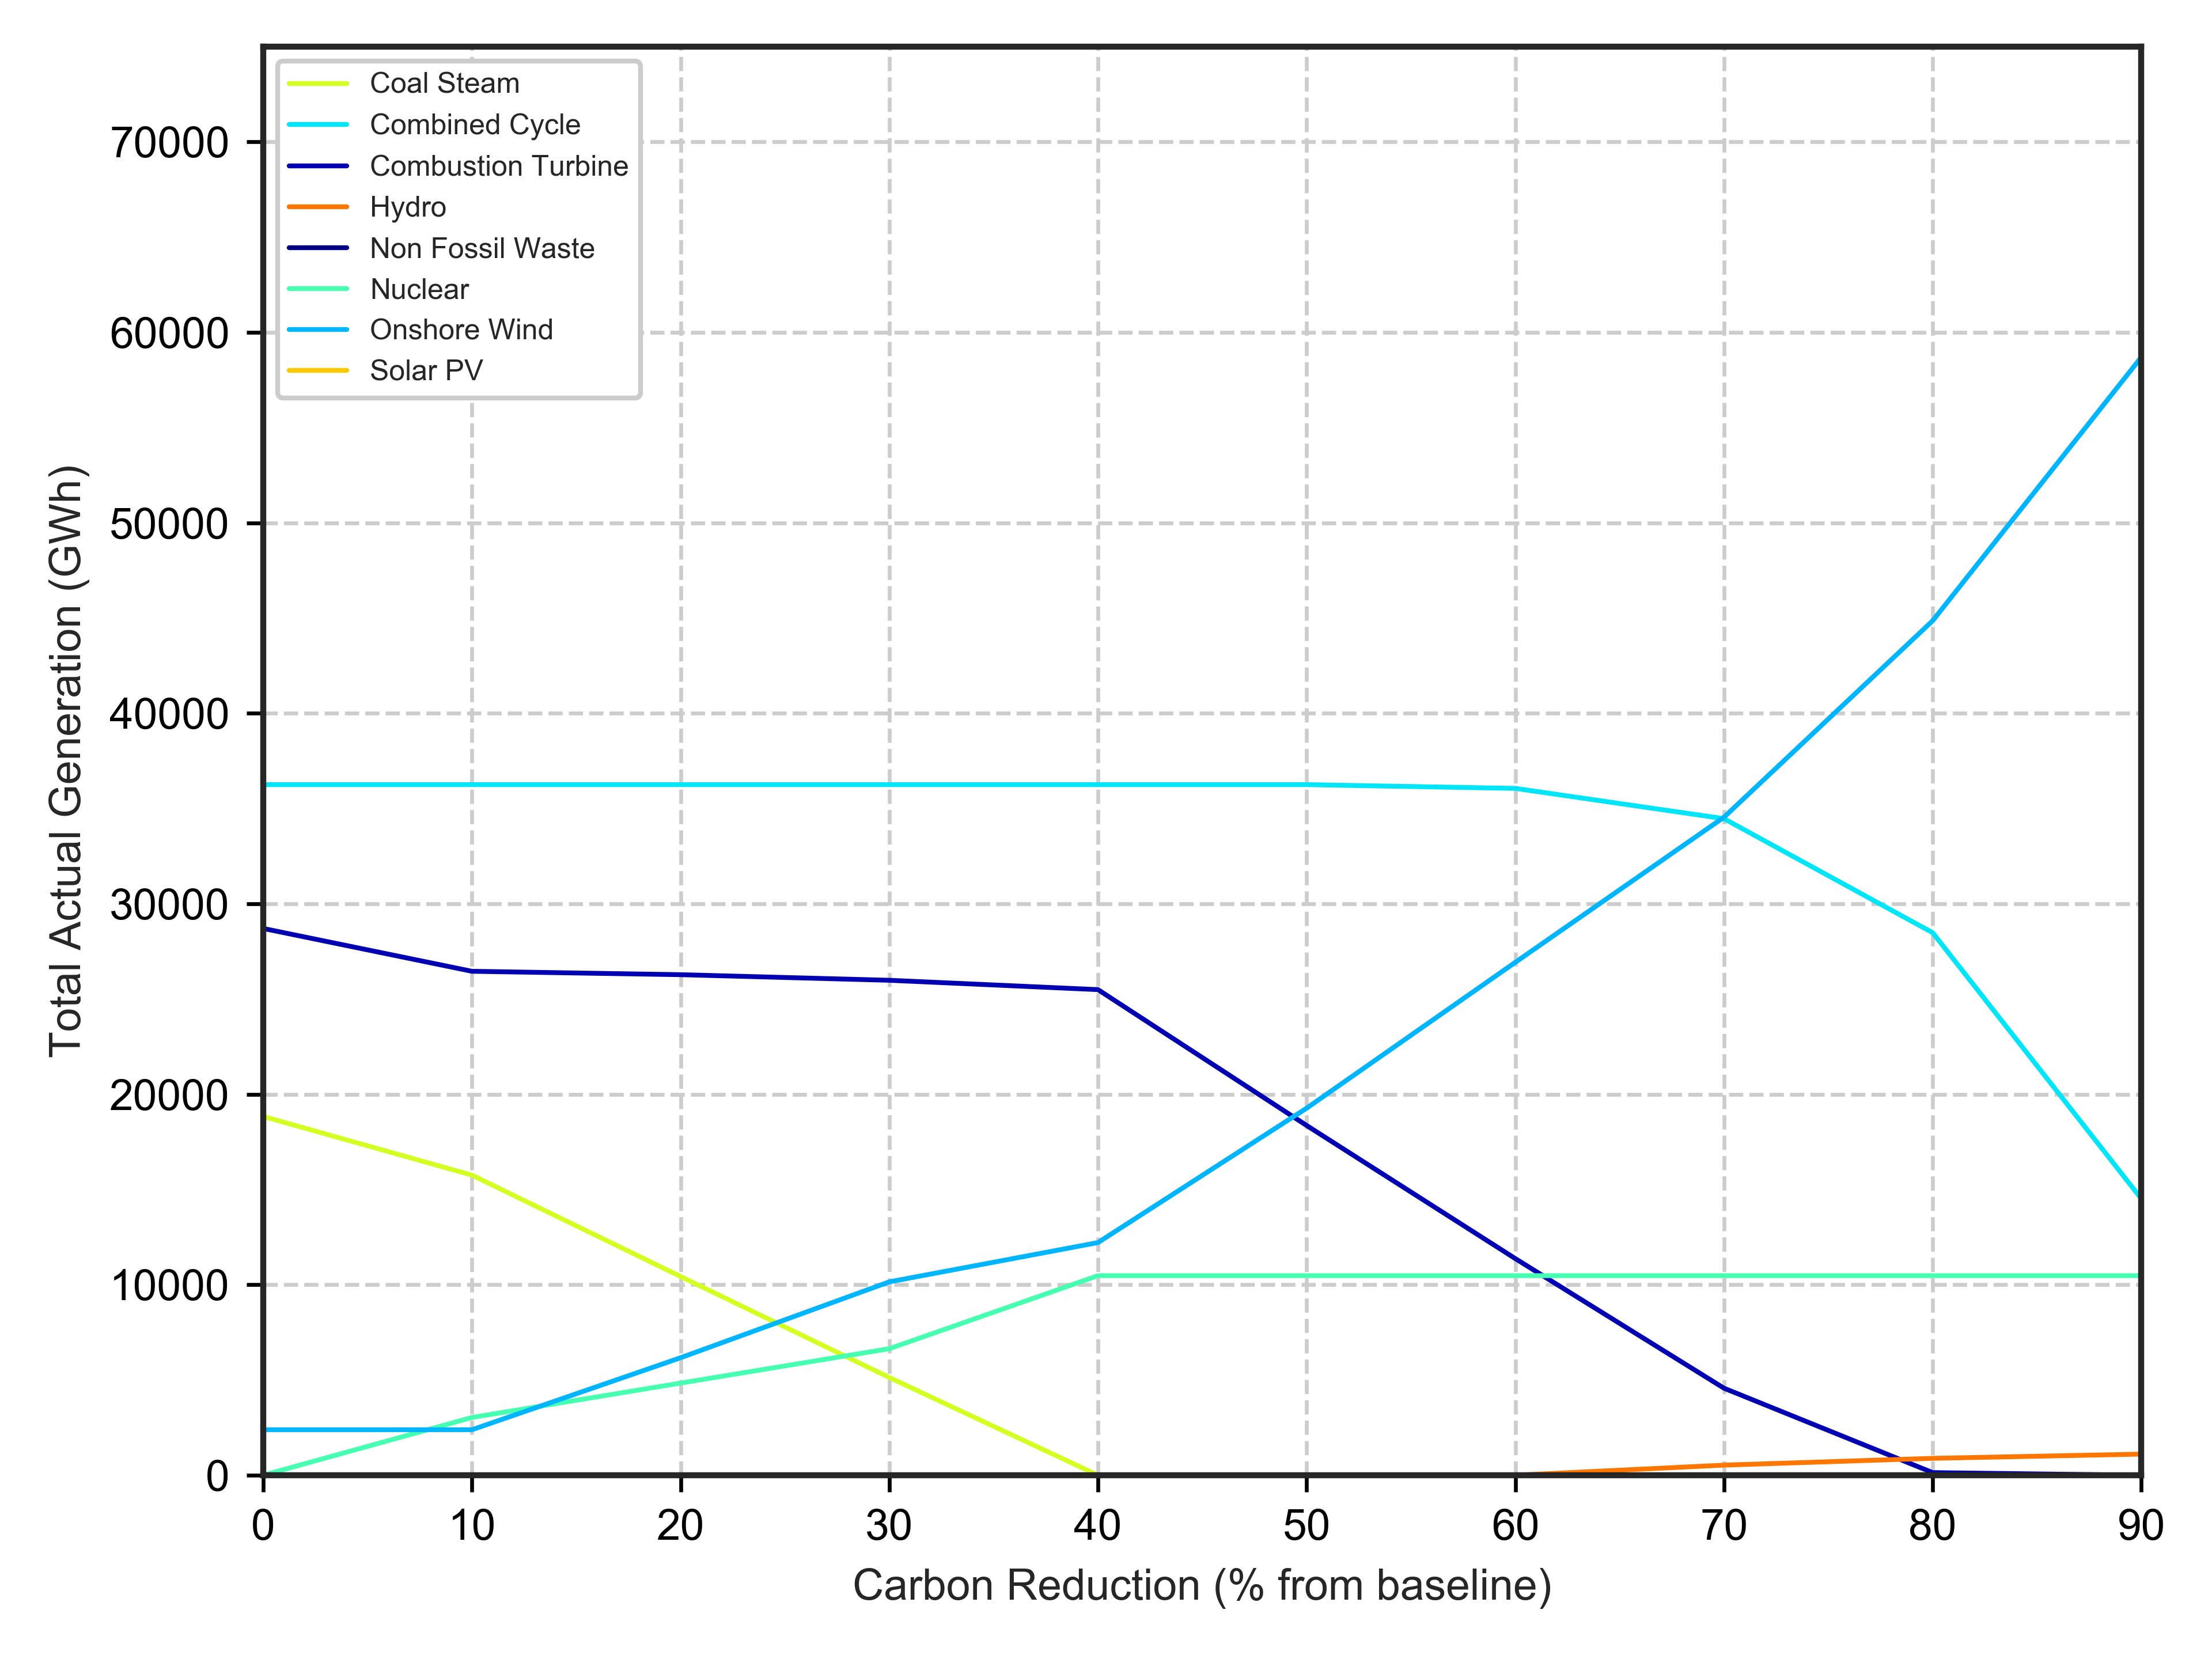
\includegraphics[width=0.32\textwidth]{includes/no_leakage_shutdowns_agg_generation_cntlreg.png}
  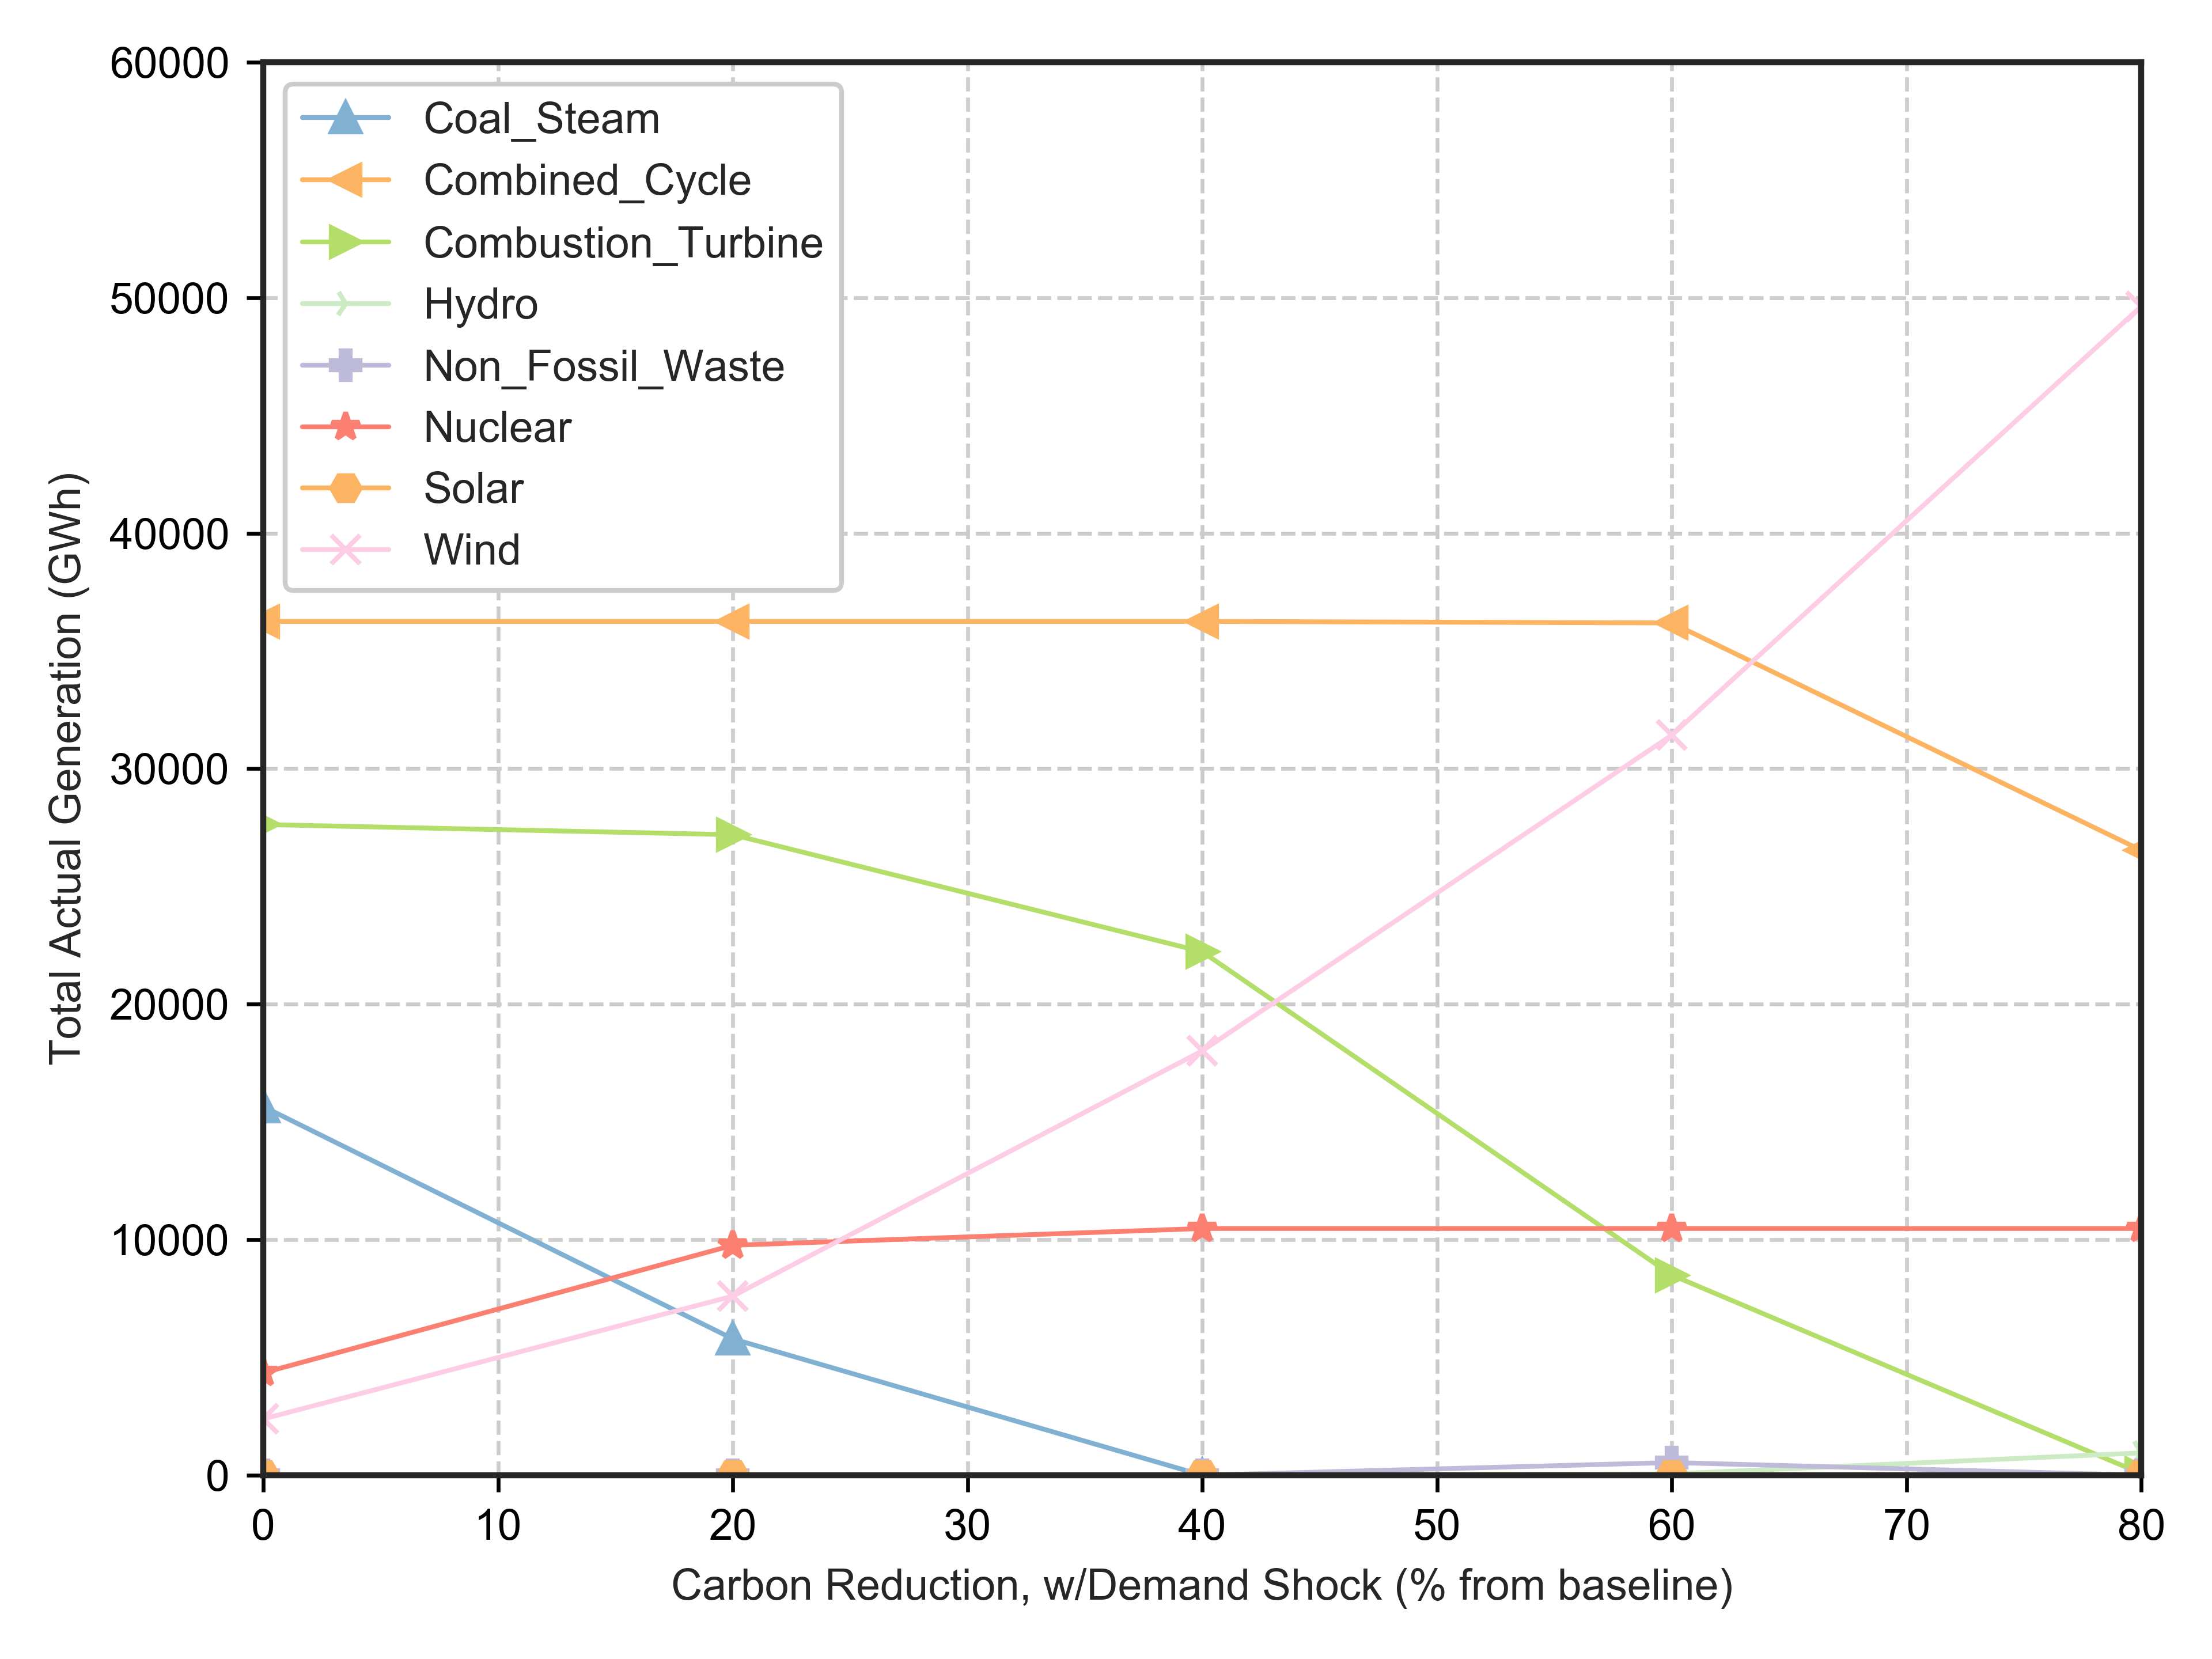
\includegraphics[width=0.32\textwidth]{includes/no_leakage_demand_shock_agg_generation_cntlreg.png}

% % this shows the increase in emissions for both control regions (WI) and non-control regions
% 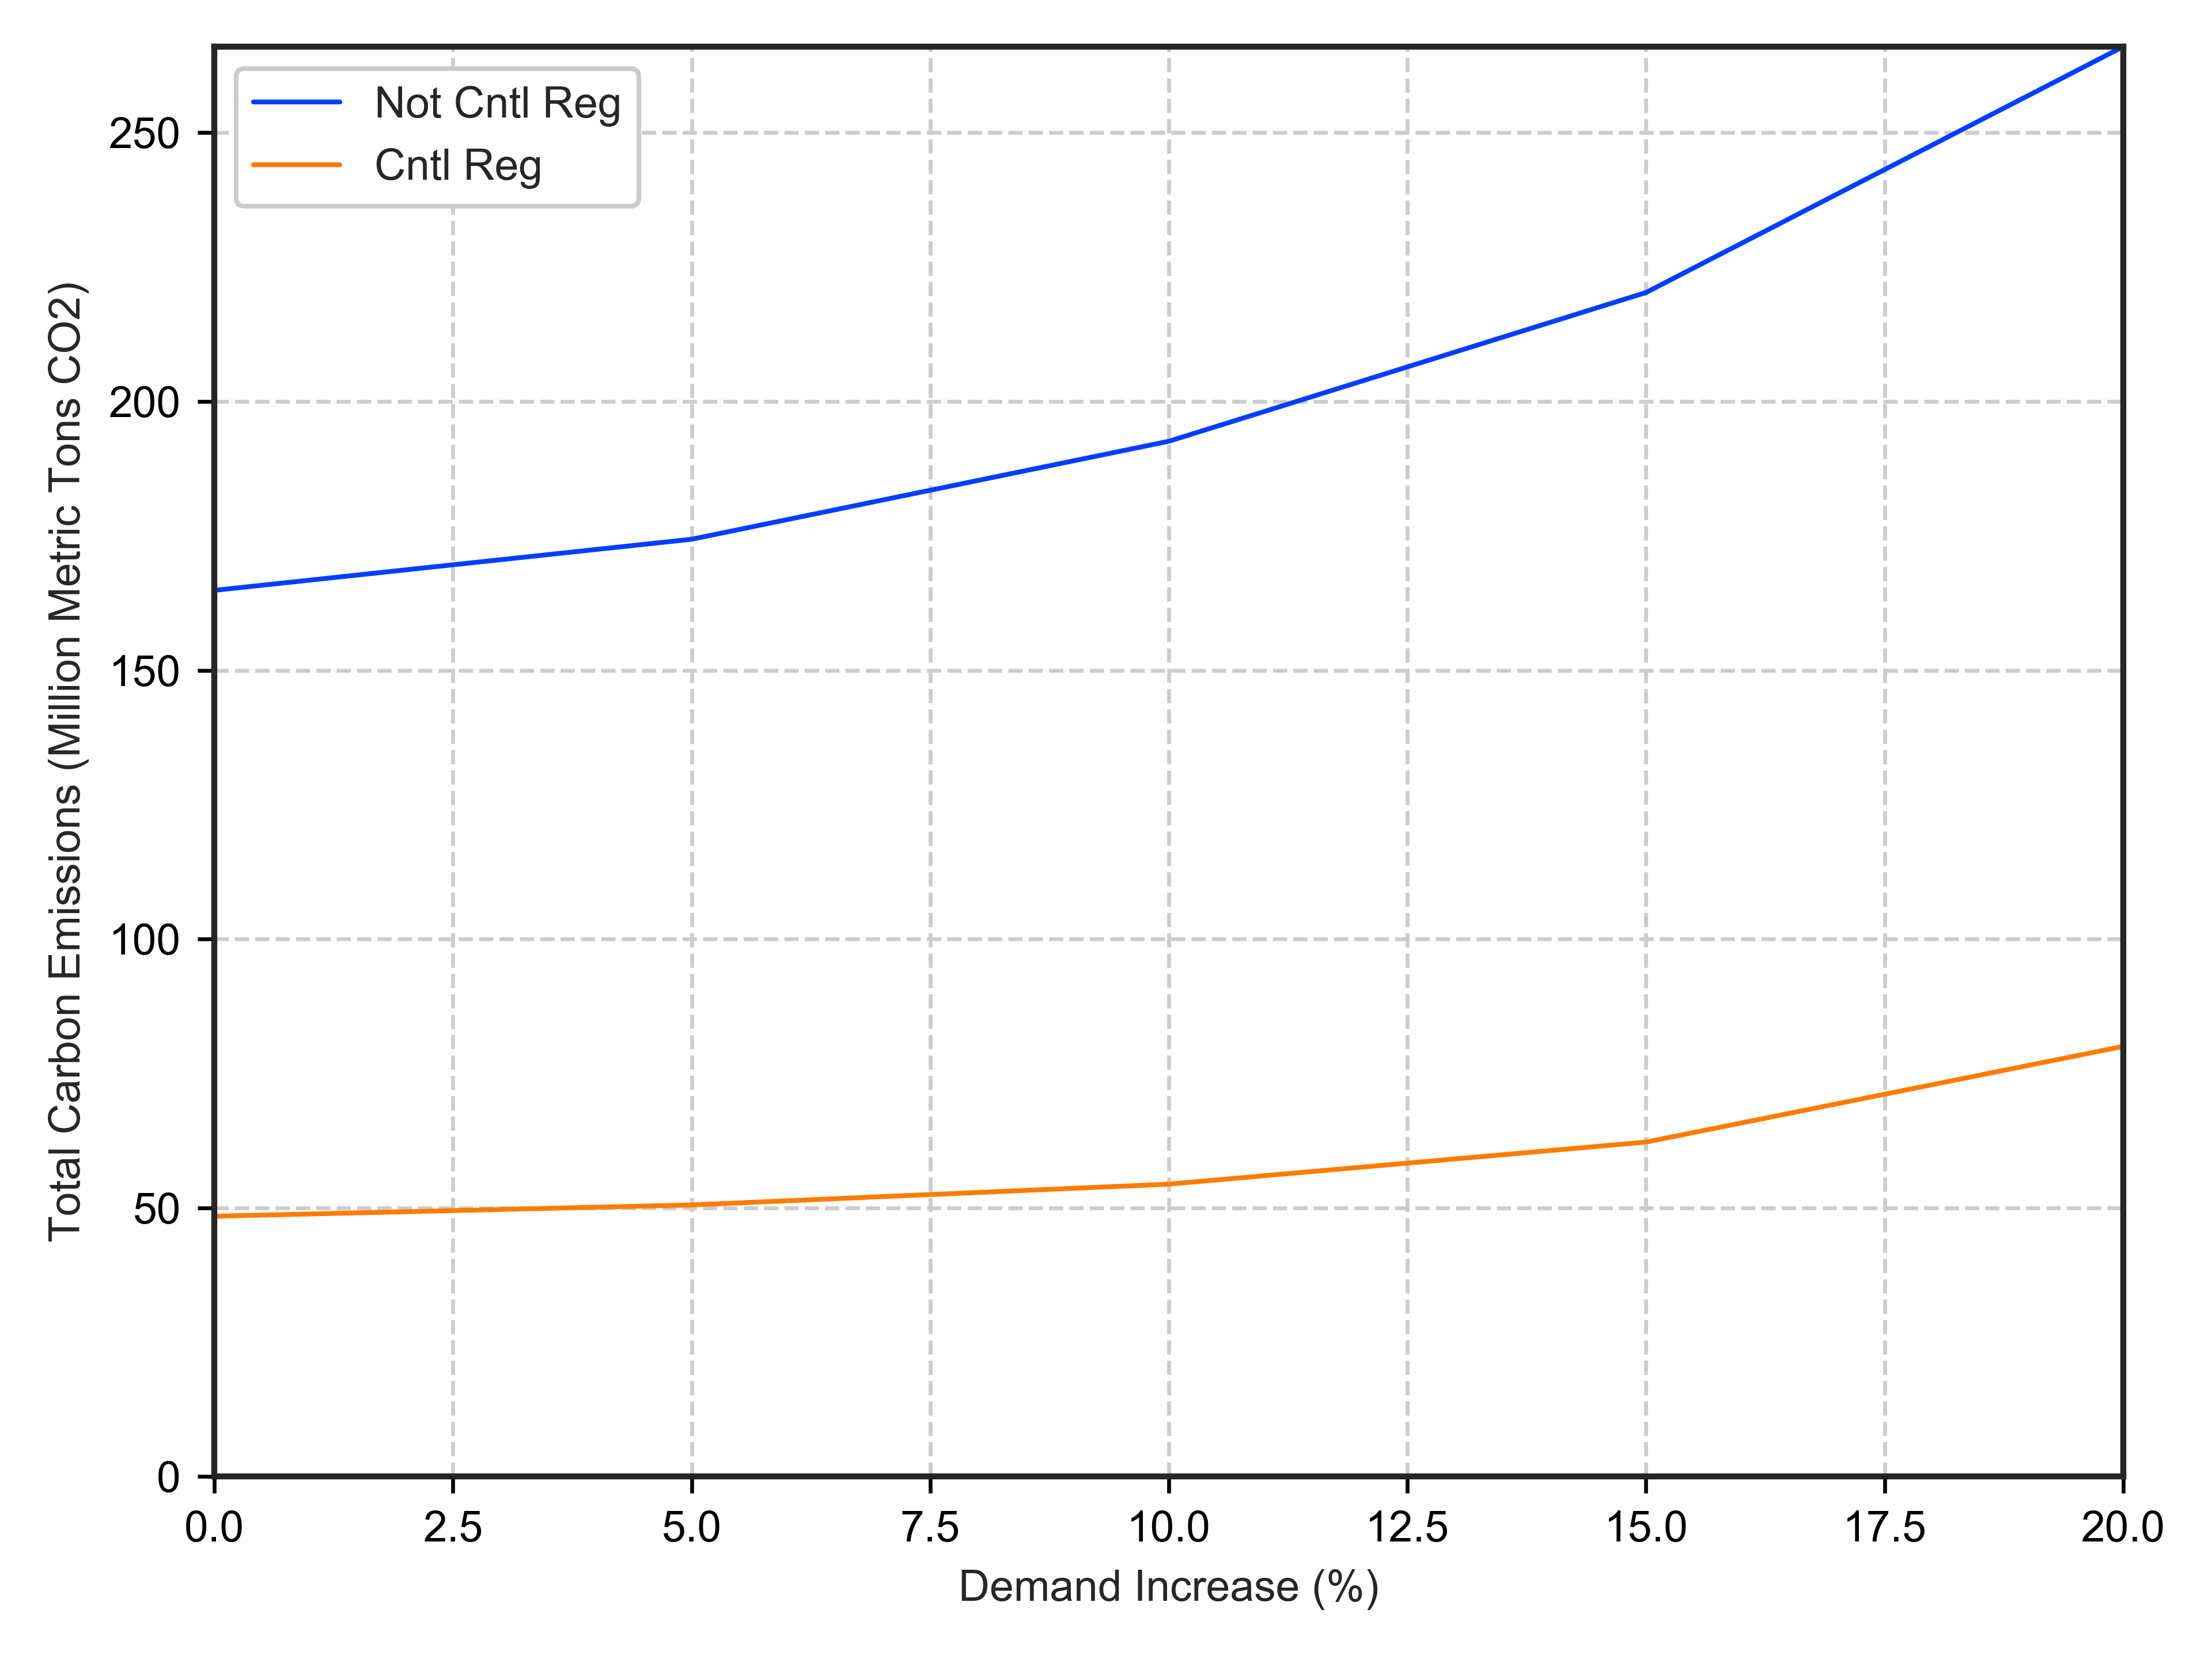
\includegraphics[width=0.20\textwidth]{includes/demand_agg_emissions.png}
%
% % shows investment costs by region (note that model is restricted to only allow investments in WI)
% 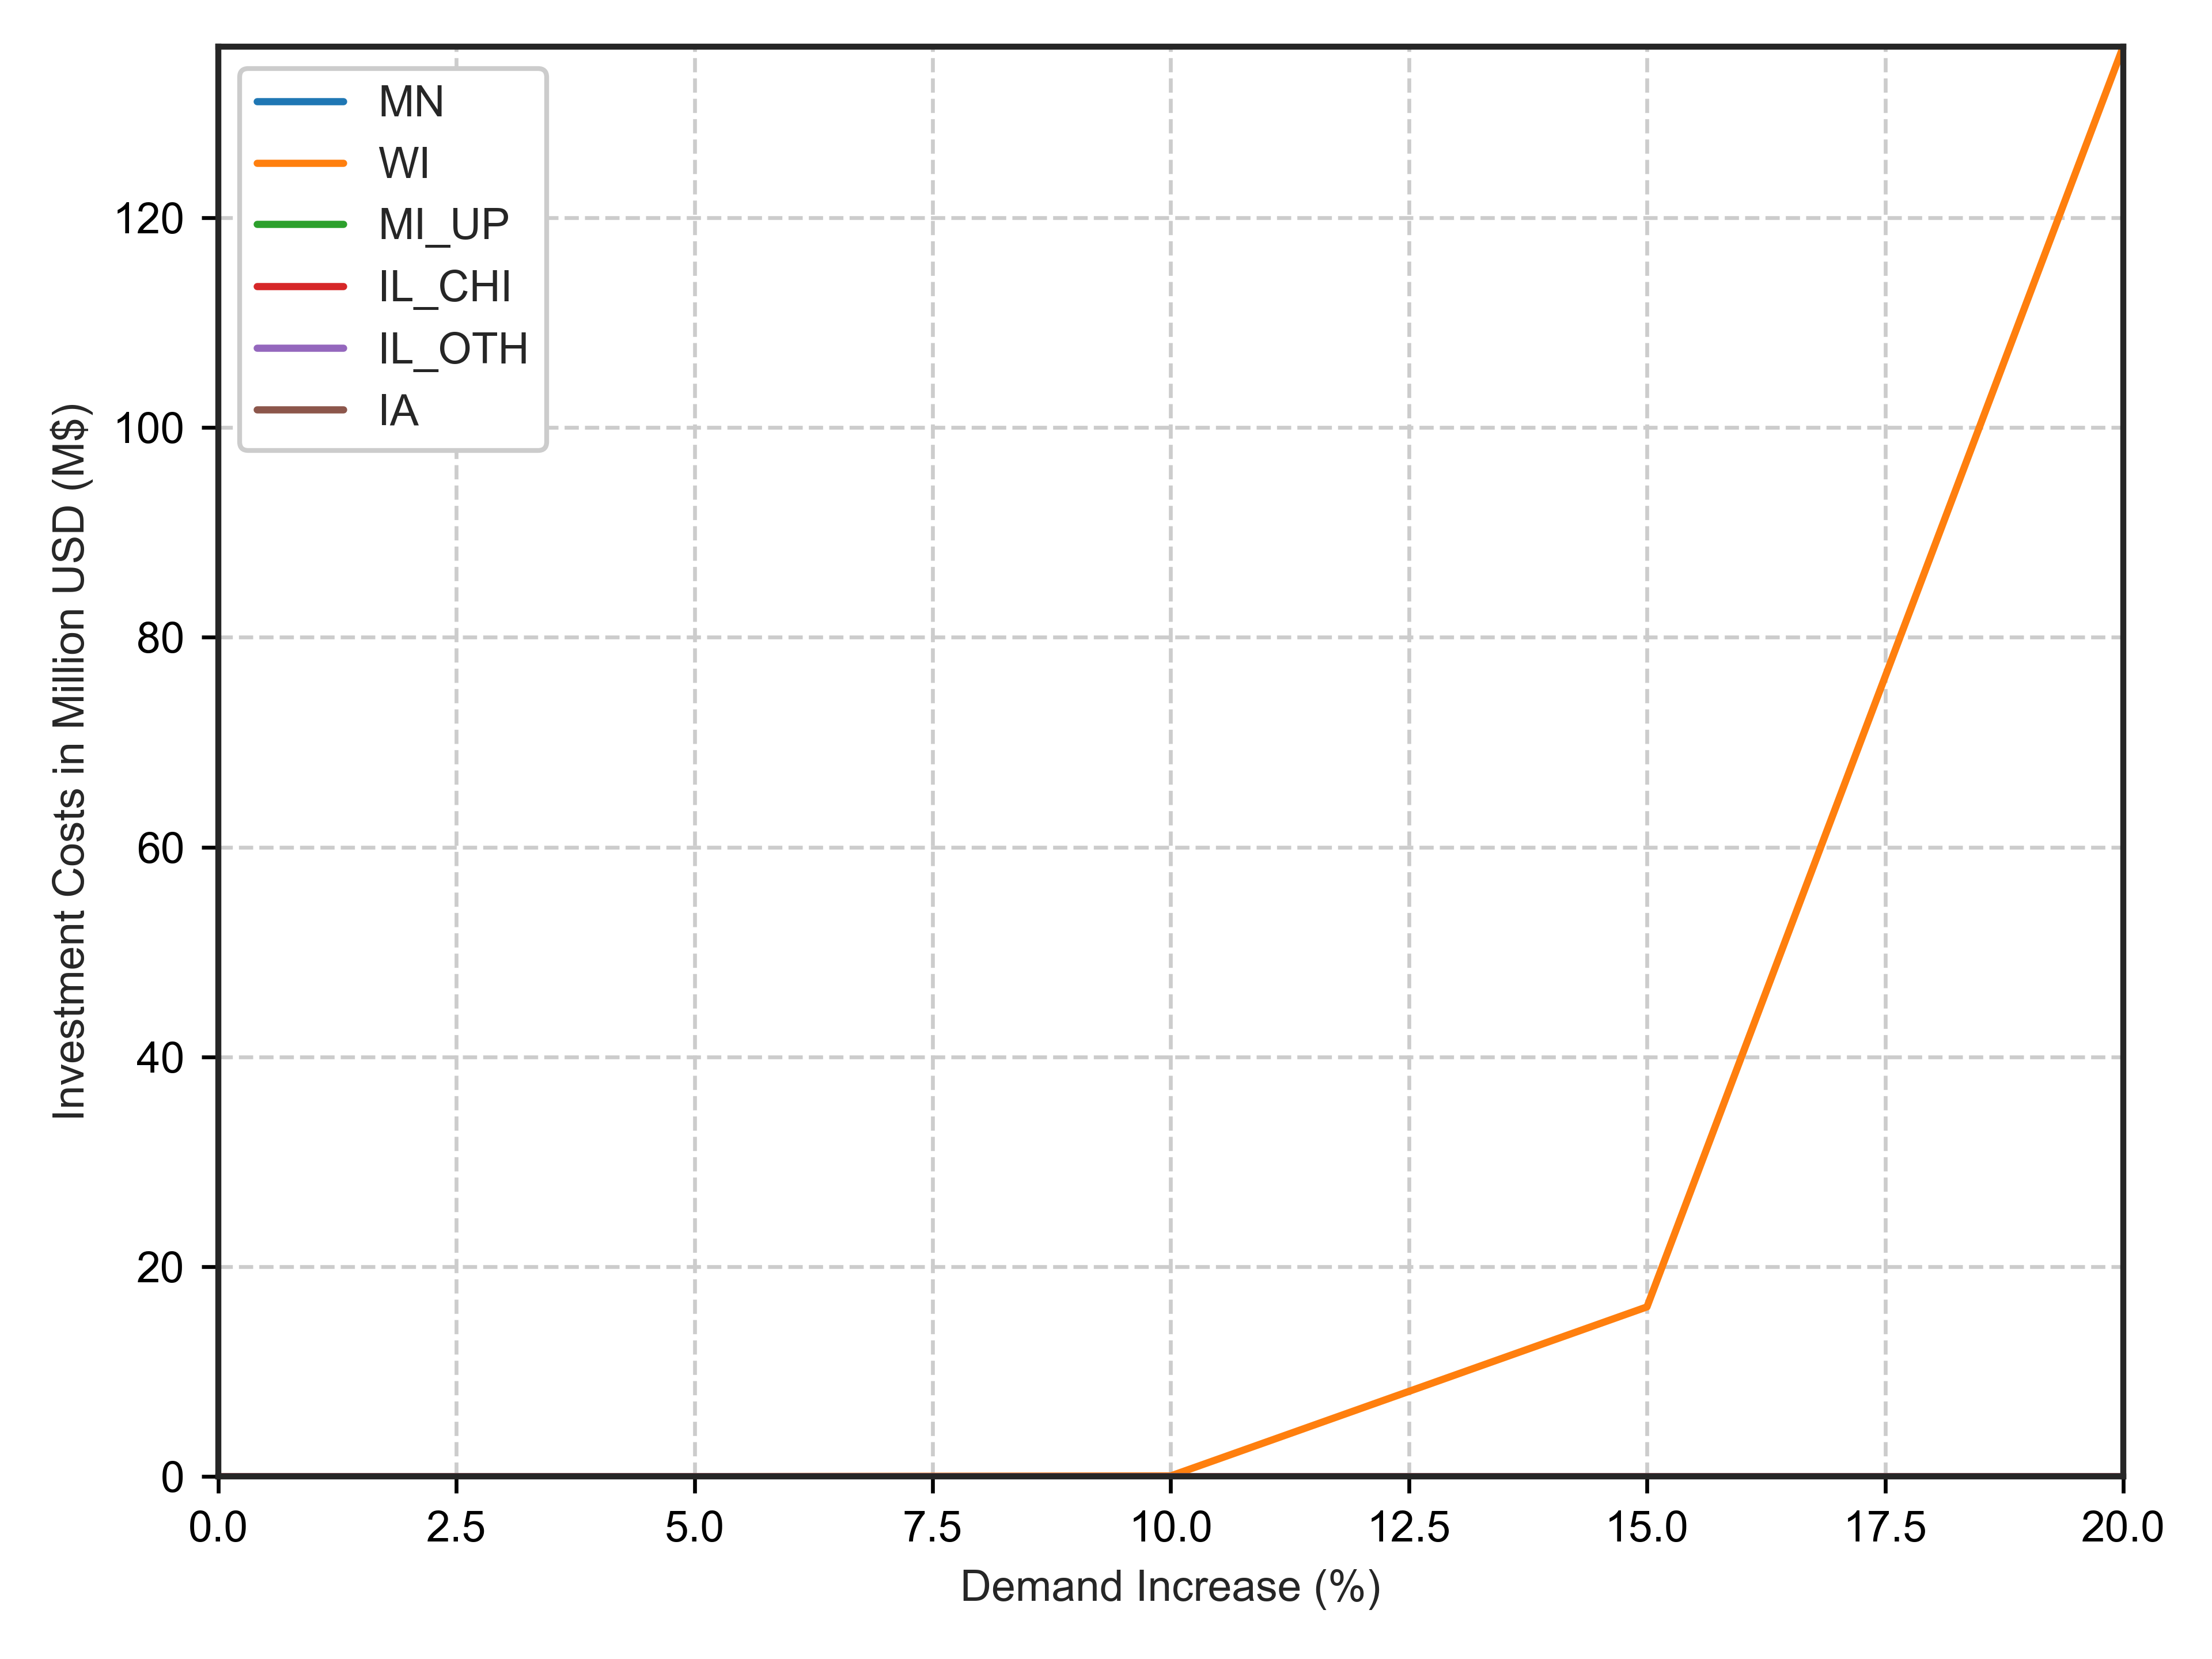
\includegraphics[width=0.20\textwidth]{includes/demand_invest_costs_by_region.png.png}
%
% % shows operational costs by region
% 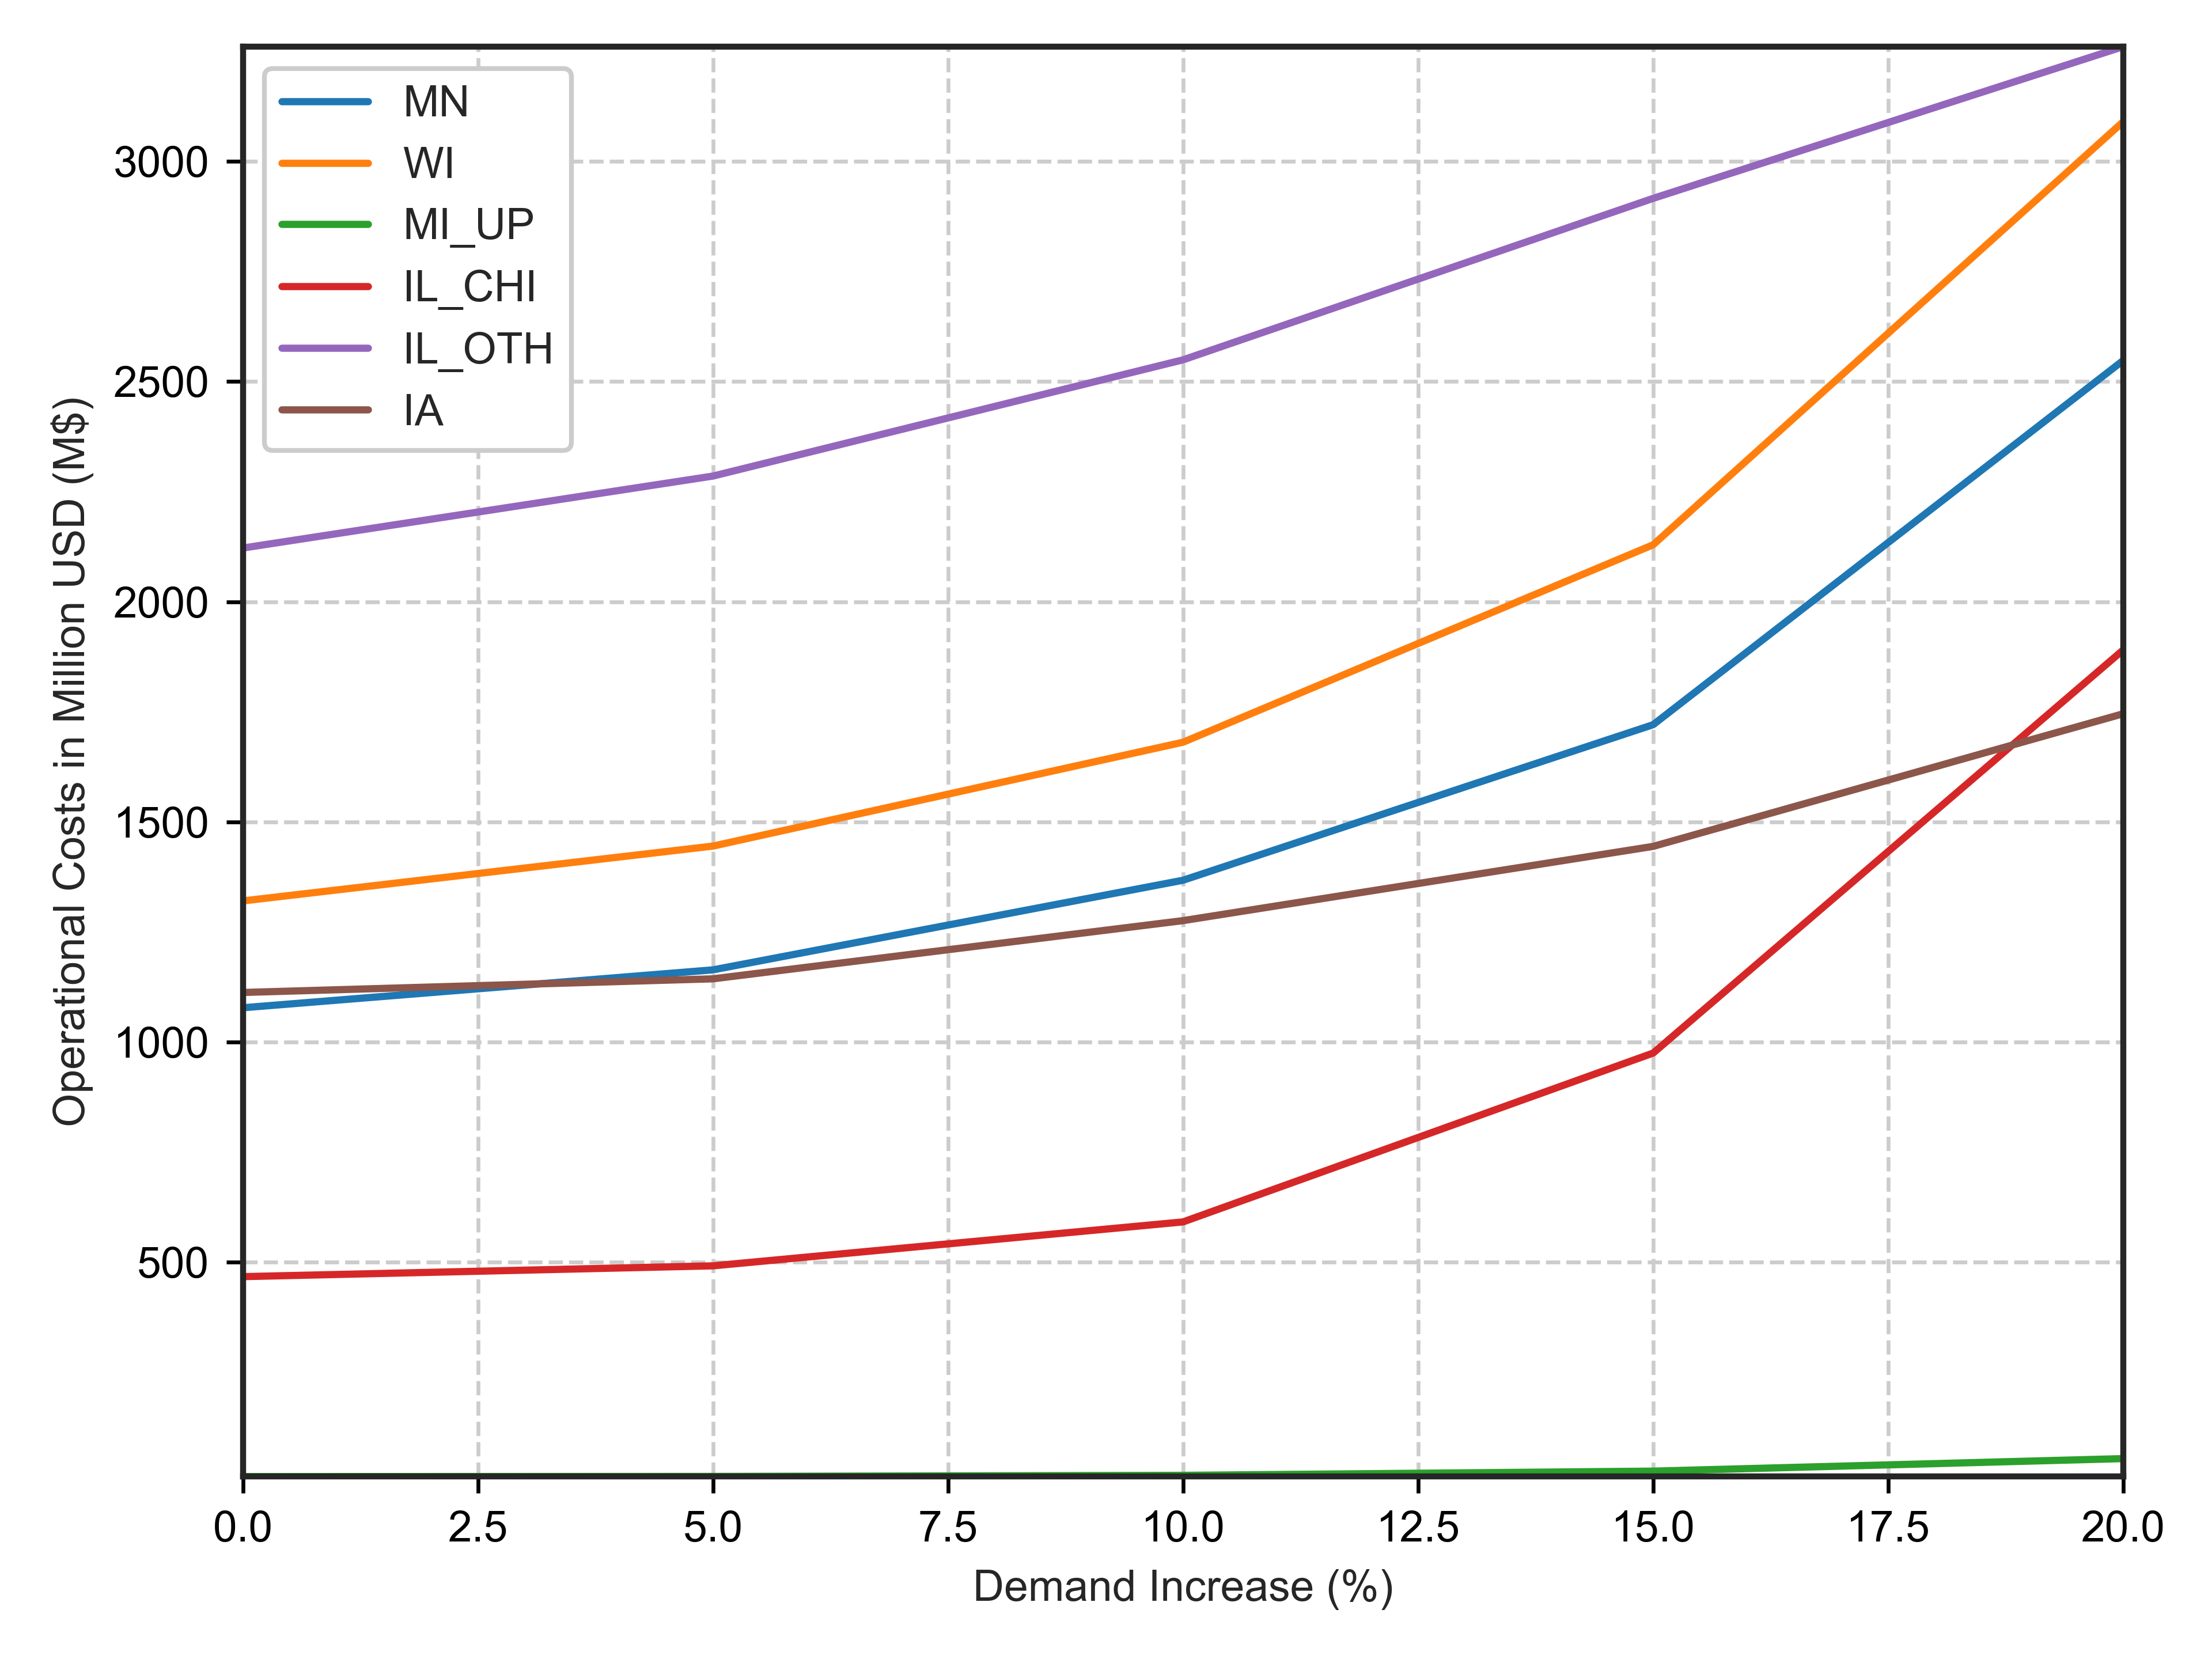
\includegraphics[width=0.20\textwidth]{includes/demand_operate_costs_by_region.png}

\end{itemize}

\end{frame}


% \begin{frame}
%   \frametitle{Environmental constraints: Capacity or CO2 reduction}
%
% Reduce capacity of plants compared to reduction in CO2 emissions. Flat imports.
% \begin{enumerate}
% \item Reduce \alert{CO2 emissions} compared with 2017:
% \item Reduce \alert{non-renewable capacity} compared with 2017:
% \item Reduce \alert{non-renewable generation} compared with 2017:
% \end{enumerate}
%
% \end{frame}
%

% \begin{frame}
%   \frametitle{Limits on technology expansion}
%
% Could limit capacity expansion on certain technologies, or could have flat imports on non-renewable generation and different limits on non-renewable imports.   Or could just limit wind and see what takes up the slack (with flat imports).
%
% \end{frame}


% THIS SLIDE SHOWS RESULTS FROM RUNS THAT DID ALLOW SHUTDOWNS
\begin{frame}
  \frametitle{Limits on technology expansion -- Shutdowns Allowed}
  Expansion of combustion turbines for 2030, but then they ramp down as capacity limit grows\\
  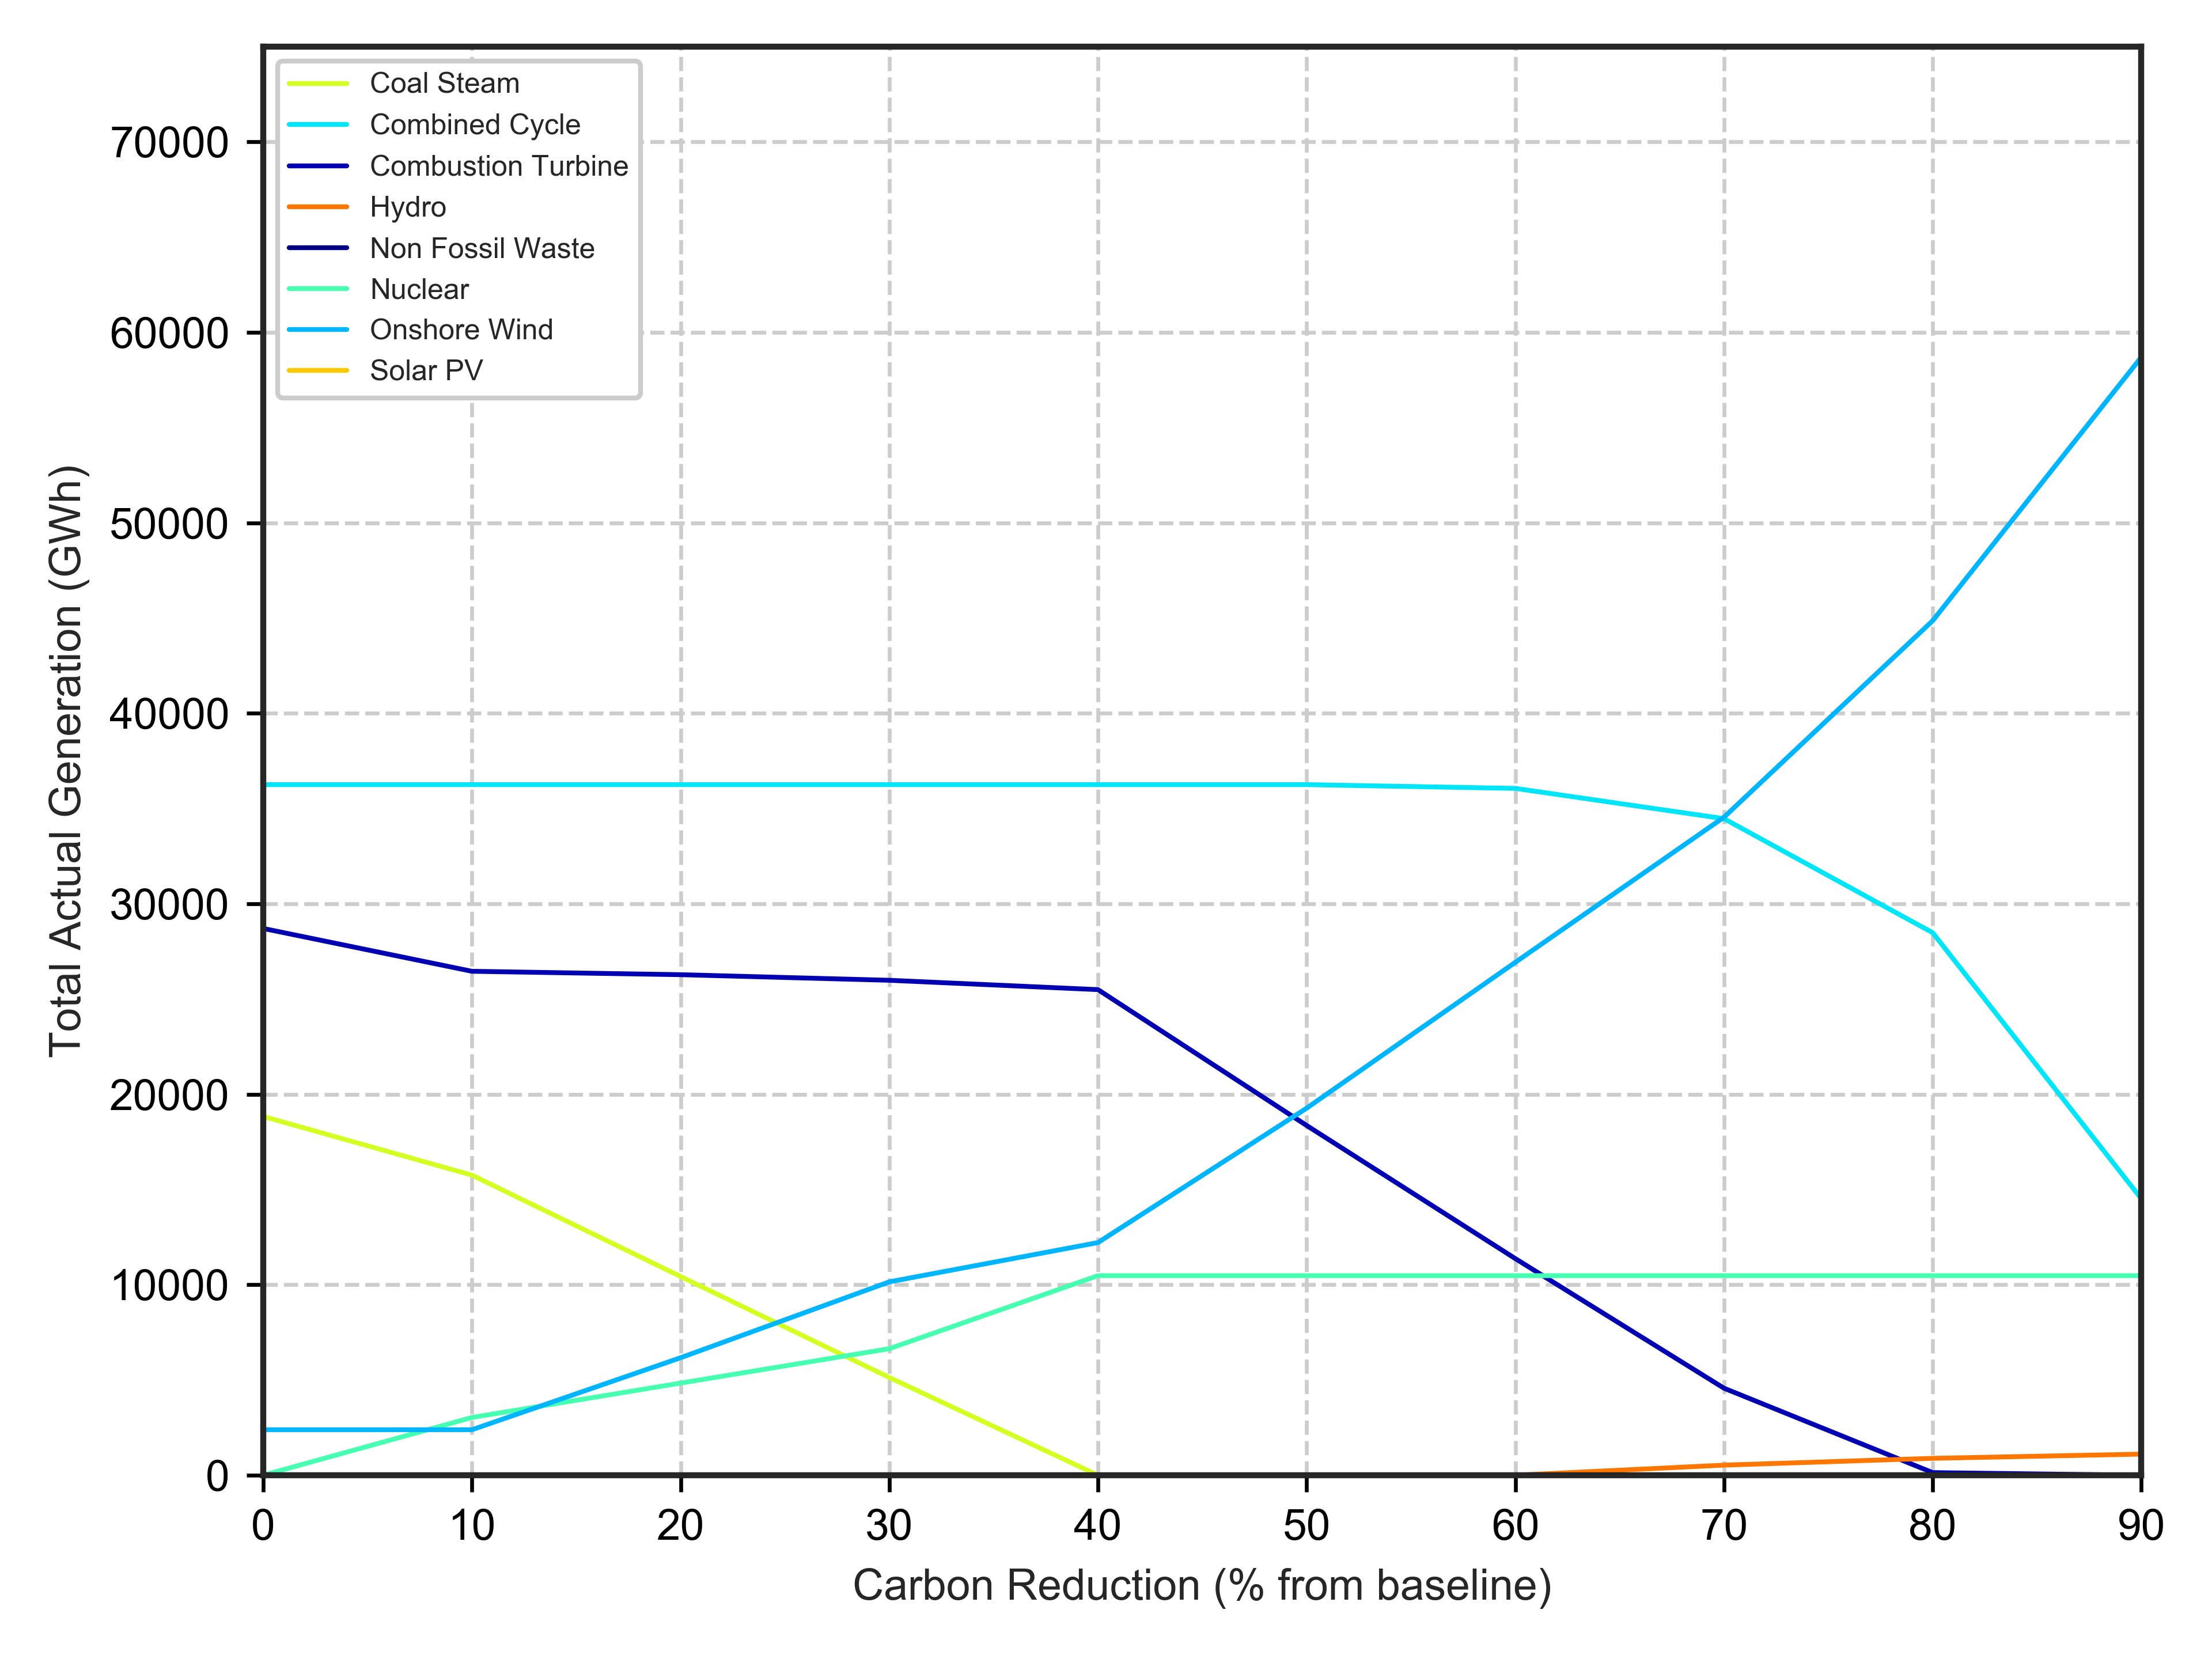
\includegraphics[width=0.32\textwidth]{includes/no_leakage_shutdowns_agg_generation_cntlreg.png}
  % this is the actual generation for the NO carbon leak scenario (WI only)
  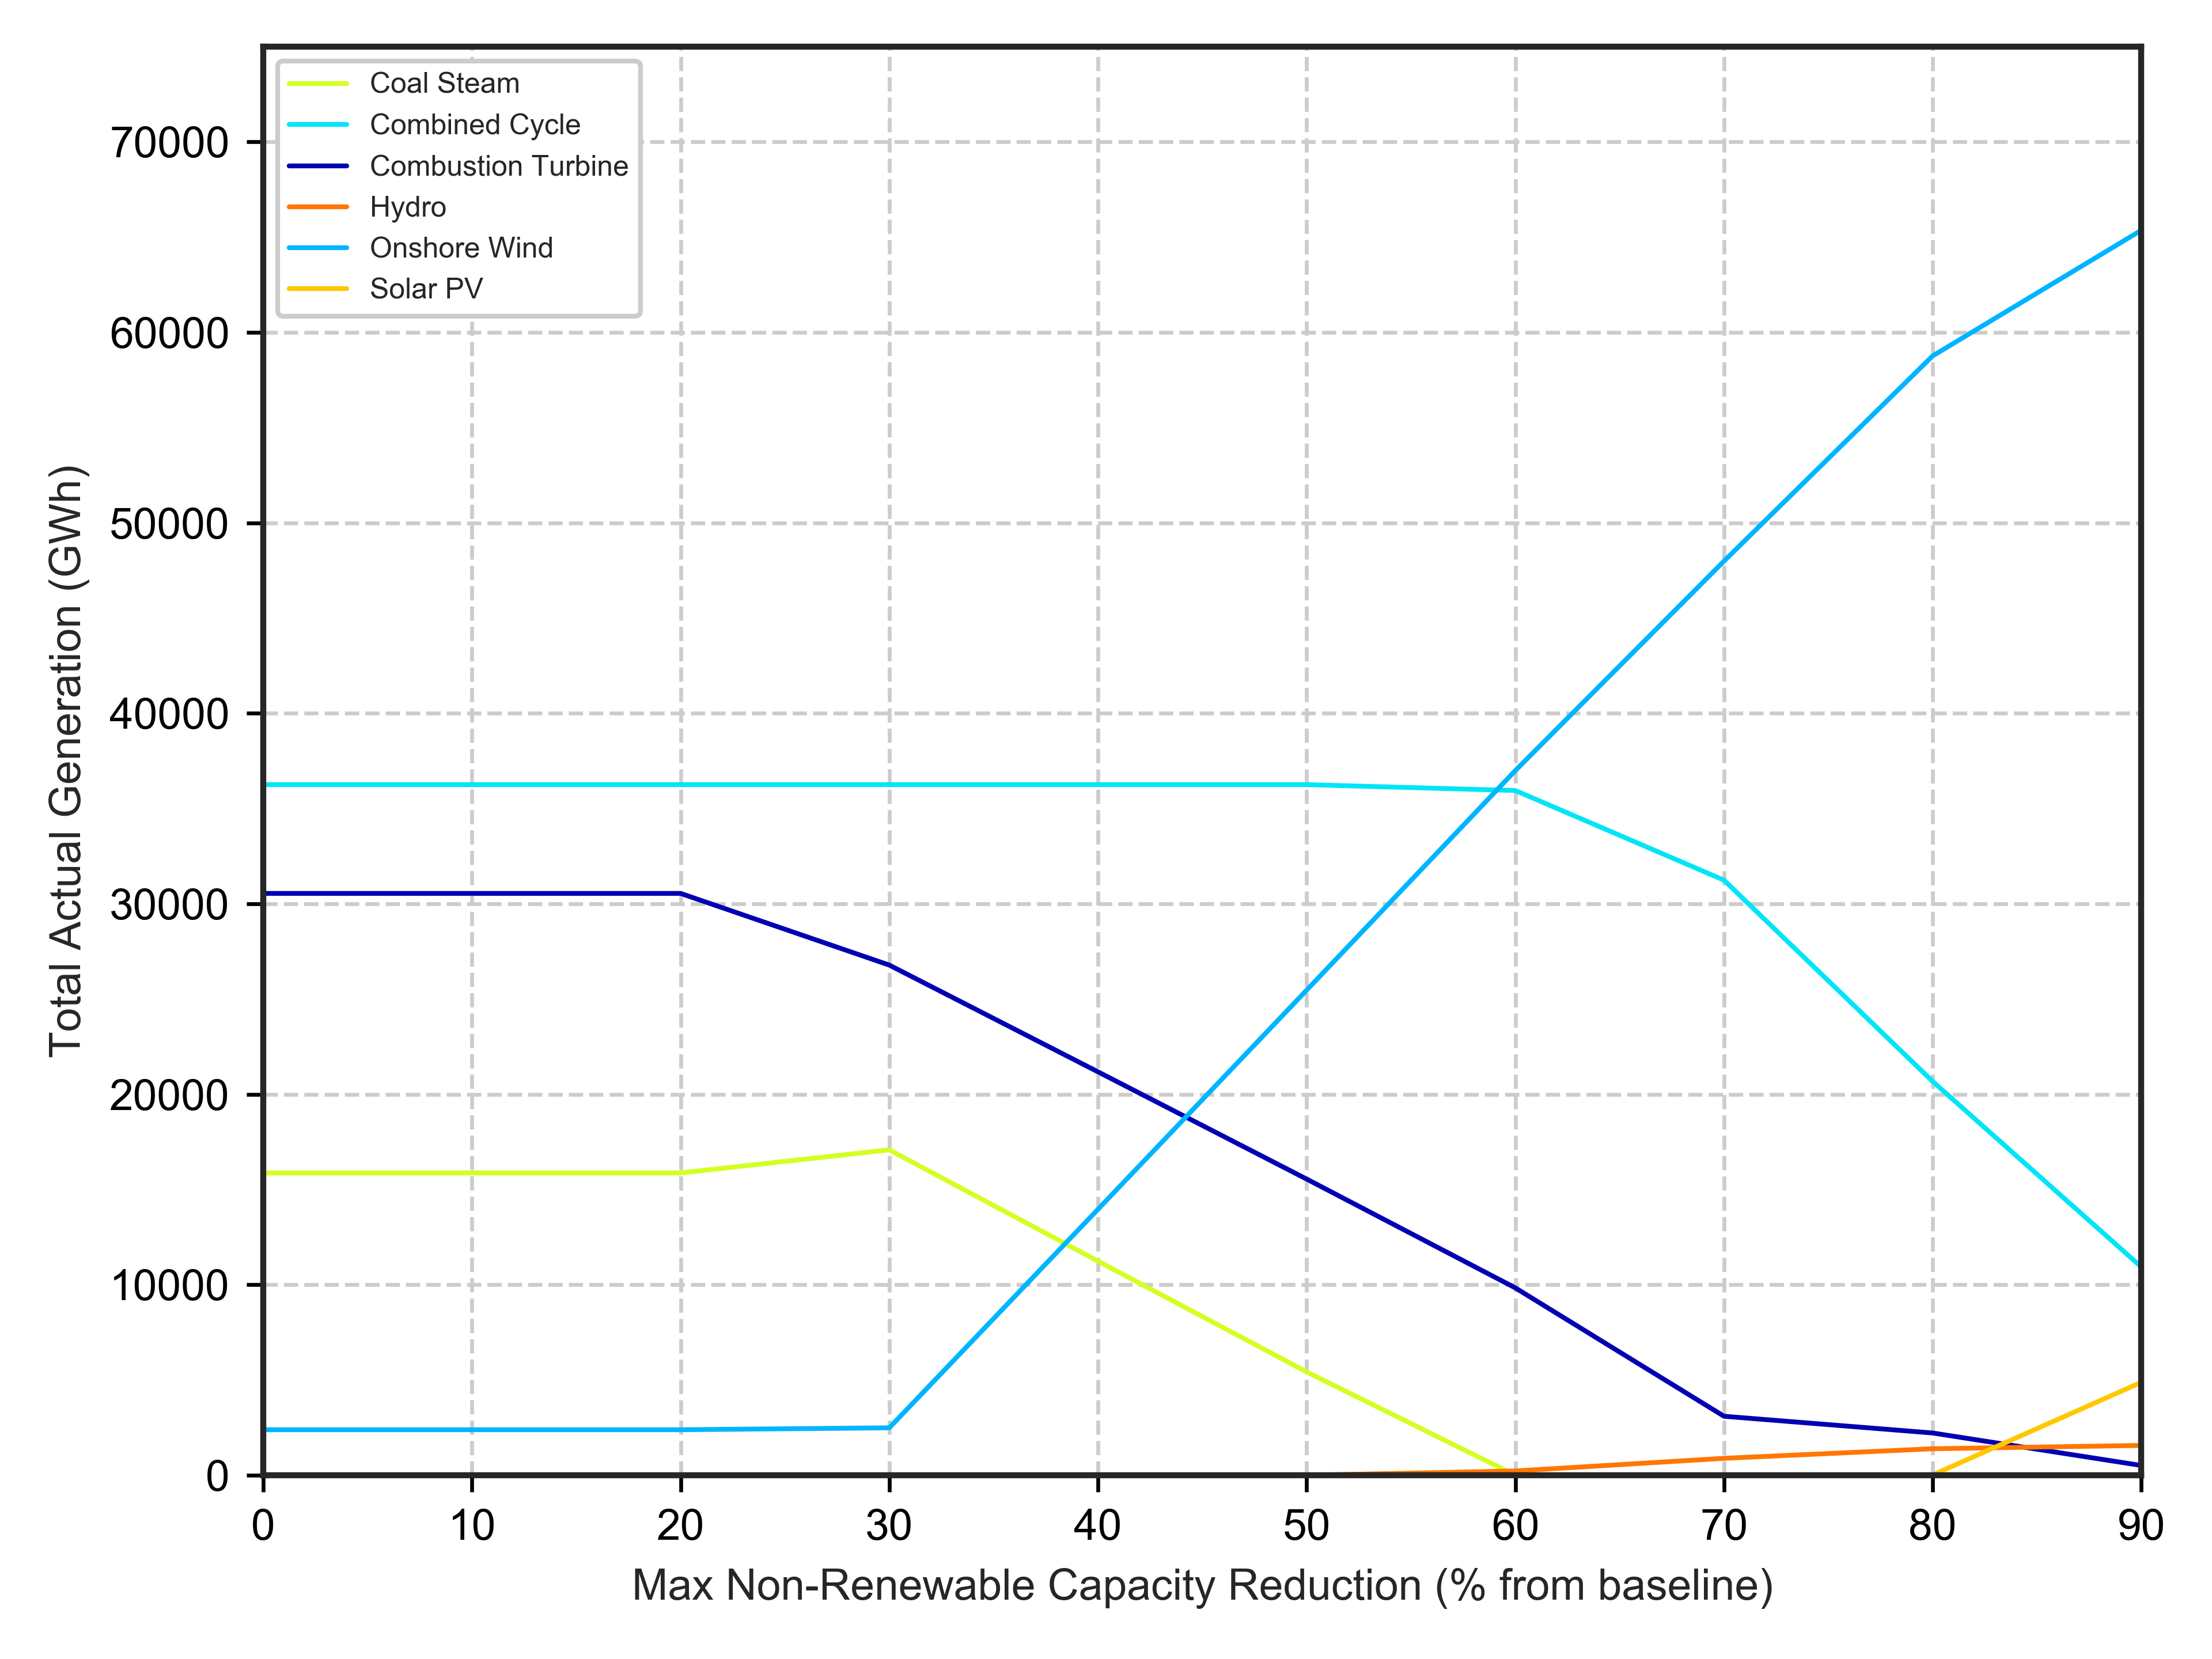
\includegraphics[width=0.32\textwidth]{includes/no_leakage_maxNR_agg_generation_cntlreg.png}
  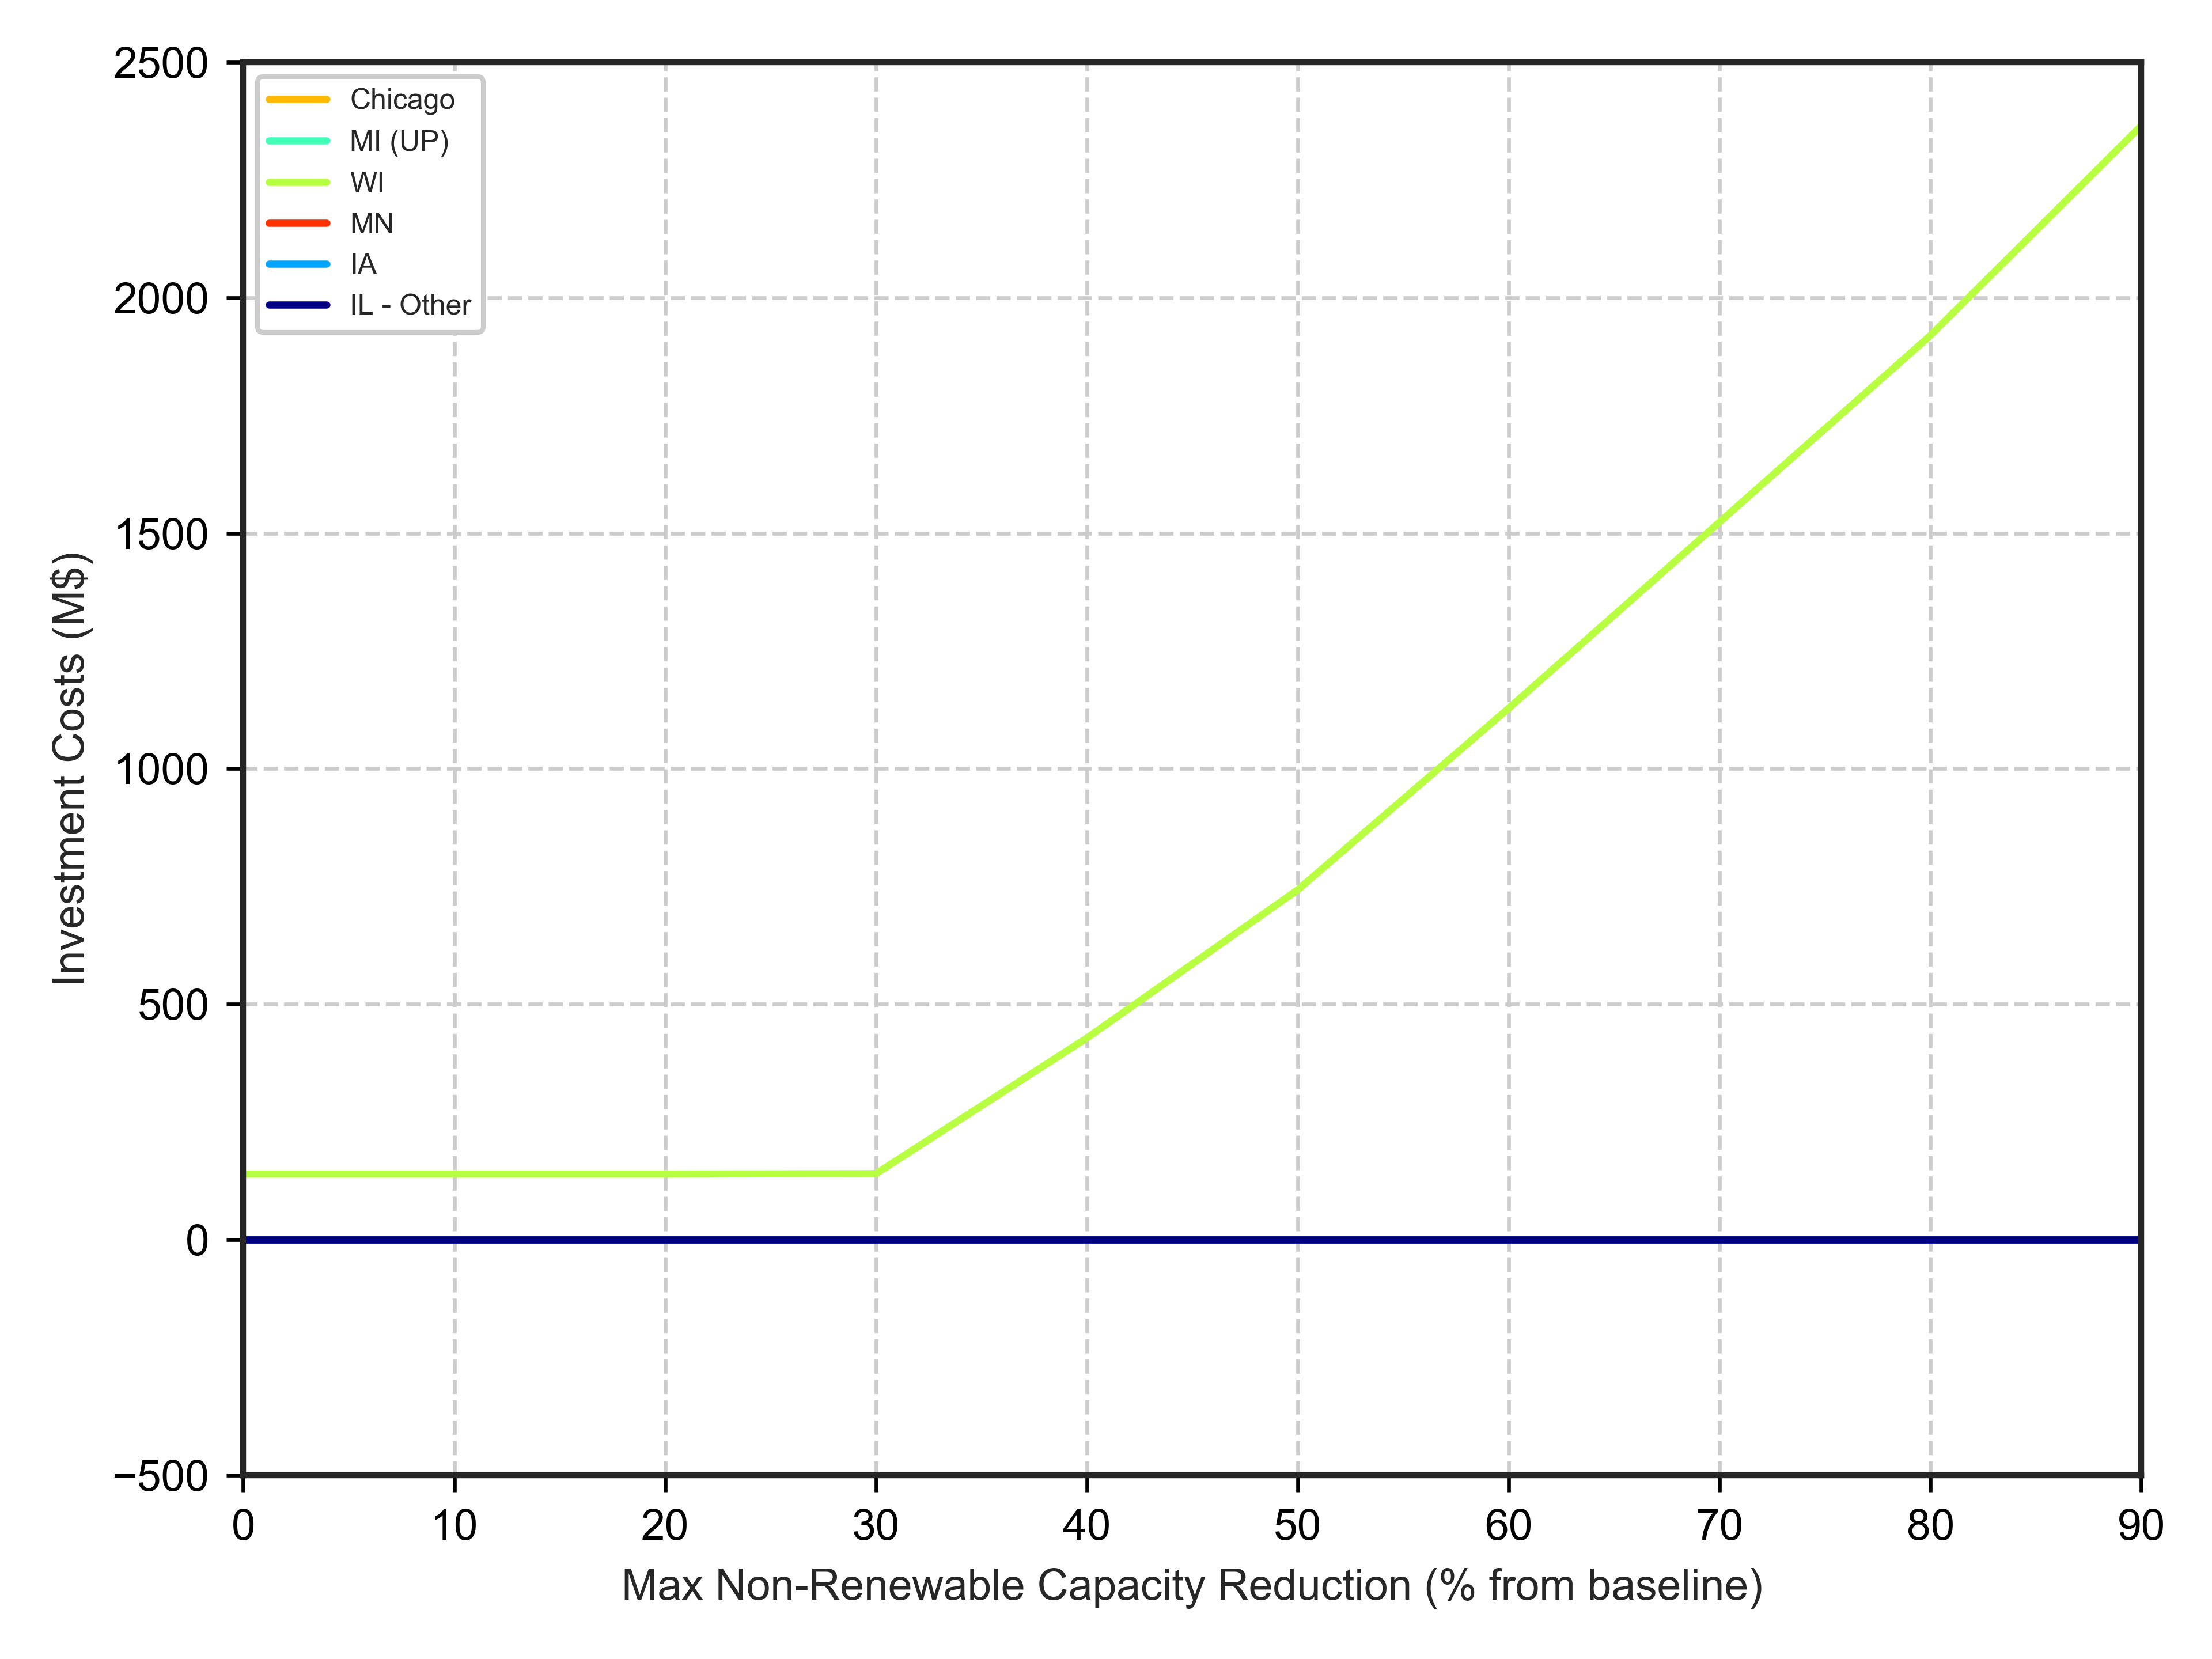
\includegraphics[width=0.32\textwidth]{includes/no_leakage_maxNR_invest_costs_by_region.png}

  Solar deployment ramps up...
  \includegraphics[width=0.25\textwidth]{includes/no_leakage_maxNR_solar_r0.png}
%  \includegraphics[width=0.25\textwidth]{includes/no_leakage_maxNR_solar_r1.png}
  \includegraphics[width=0.25\textwidth]{includes/no_leakage_maxNR_solar_r2.png}
  \includegraphics[width=0.25\textwidth]{includes/no_leakage_maxNR_solar_r3.png}
  \includegraphics[width=0.25\textwidth]{includes/no_leakage_maxNR_solar_r4.png}

\end{frame}

\begin{frame}

  \begin{itemize}
  \item Policy Experiment - limit capacity expansion on all non-renewable technologies.
  \item Can expect huge increases in solar and wind, but where?
  \item Model does not consider nuclear as a renewable technology in this experiment

  \item Investment costs for WI
    \includegraphics[width=0.2\textwidth]{includes/no_leakage_maxNR_invest_costs_by_region.png}

\end{itemize}
\end{frame}

\begin{frame}
  \frametitle{Conclusions}
  \begin{itemize}
  \item Models can inform policy
  \item Models can show effects and costs of constraints
  \item Investment is coupled to reliability
      \item The model is currently being refined, and we are interested to get feedback from utility and policy experts about how this model would be useful in your utility and regulatory planning efforts (by April-May)
  \item  here's how to get in touch with us if you should be interested in a one-on-one demonstration of the model and/or a brief interview to discuss possible policy interventions - we would anticipate after this first round of WEREWOLF (funded by TT Center) that we will be exploring additional opportunities to partner with stakeholders to further evolve the model with the goal of making it as useful as possible to policy stakeholders (such as through ARPA-E or other funding sources down the road).
  \end{itemize}
\end{frame}
%
% \appendix
%
% \begin{frame}
% In the Appendix, you could include information about the model (the
% current slides 4, 5) for example.
% \begin{itemize}
%   \item \color{black} Very large scale models (many agents with many instruments
%     acting strategically) with risk are hard
%   \item \alert{New algorithms enable solution of more detailed,
%       authentic problems and address underlying policy questions}
%   \item Evaluation via simulation computations and out-of-sample testing
% \end{itemize}
% \end{frame}
%
%
% \begin{frame}
%   \frametitle{Technology choices as $\theta$ increases (NR capacity redn)}
%
%   \includegraphics[width=4.8in]{includes/Scaprednv20.png} \\
% %\makebox[\linewidth]{\includegraphics[clip,trim=0.1cm 0.2cm 0.1cm
% %  1.6cm,page=30,width=5.2in]{OFBPhilpottv2.pdf}}
%   \begin{itemize}
%   \item Use geothermal, CCS, wind, batteries
%   \item Fairly constant capacity
%   \end{itemize}
% \end{frame}
%
% \begin{frame}
%   \frametitle{Technology choices as $\theta$ increases (\% CO2 redn)}
%
%   \includegraphics[width=4.8in]{includes/Sco2rednv20.png} \\
% %\makebox[\linewidth]{\includegraphics[clip,trim=0.1cm 0.2cm 0.1cm
% % 1.6cm,page=30,width=5.2in]{OFBPhilpottv2.pdf}}
%   \begin{itemize}
%   \item Rich portfolio of renewable technologies used
%   \item More capacity needed as more uncertain generation
%   \end{itemize}
% \end{frame}
%
% \begin{frame}
%   \frametitle{Technology choices as carbon price (\$ per MW) increases}
%
%   \includegraphics[width=4.8in]{includes/Sco2incrv20.png}
% %\makebox[\linewidth]{\includegraphics[clip,trim=0.1cm 0.2cm 0.1cm
% %  1.6cm,page=30,width=5.2in]{OFBPhilpottv2.pdf}}
% \end{frame}
%
% \begin{frame}
%   \frametitle{CO2 reduction (constraint or carbon tax)}
%
%     \includegraphics[width=0.5\textwidth]{includes/TotalCarbonSinglev20.png}
%     \includegraphics[width=0.5\textwidth]{includes/TotalCarbonincrv20.png}
%
% \end{frame}
%
% \begin{frame}
%   \frametitle{Technologies (chance constraints):
%     cf. increased uptake}
%
% \centering
% Force zero emissions in at least 50\% of years (normal hydrology)\\
% \includegraphics[clip,trim=1.25cm 0.95cm 0.0cm 0.0cm,height=2.8cm]{includes/SccConstraint.png}
% \includegraphics[clip,trim=1.25cm 0.95cm 5.1cm 0.0cm,height=2.8cm]{includes/SccConstraintv20.png}\\
%   \includegraphics[width=0.4\textwidth]{includes/CCvalues.png}\qquad
%   \includegraphics[width=0.4\textwidth]{includes/CCvaluesv20.png}\\
%
%   Nonzero CO$_{2}$ emissions in 6 out of the 13 scenarios\\
%   Average level of CO$_{2}$ emissions (0.138 Mt) or approx 95.4\% redn
%
% \end{frame}

\end{document}
